\documentclass[11pt]{article}

% The four macros of the header standard; tools/zenodo/publish_revision.py patches them when it reserves the DOI.
\newcommand{\doctype}{Preprint}
\newcommand{\docversion}{v1.00.000}
\newcommand{\docdate}{4 November 2026}
\newcommand{\versiondoi}{10.5281/zenodo.0}
\newcommand{\conceptdoi}{10.5281/zenodo.0}
\newcommand{\docidentity}{CAOS\_Contraste, the validation of the risk models of a bank}

% The packages and conventions every Contraste manuscript shares (CAOS_MANAGE conventions/manuscript-content-bar.md
% section 2). A document sets its class, the four header macros and \docidentity, then % The packages and conventions every Contraste manuscript shares (CAOS_MANAGE conventions/manuscript-content-bar.md
% section 2). A document sets its class, the four header macros and \docidentity, then % The packages and conventions every Contraste manuscript shares (CAOS_MANAGE conventions/manuscript-content-bar.md
% section 2). A document sets its class, the four header macros and \docidentity, then \input{../_shared/preamble}.
\usepackage[T1]{fontenc}
\usepackage[utf8]{inputenc}
\usepackage{lmodern}
\usepackage{microtype}
\usepackage[a4paper,margin=2.5cm]{geometry}
\usepackage{amsmath,amssymb,amsthm,mathtools,bm}
\usepackage{graphicx}
\usepackage{booktabs,longtable,tabularx,array,multirow}
\usepackage{siunitx}
\usepackage{algorithm}
\usepackage{algpseudocode}
\usepackage{caption,subcaption}
\usepackage{xcolor}
\usepackage[numbers,sort&compress]{natbib}
\usepackage[hidelinks]{hyperref}
\usepackage{cleveref}
\usepackage{orcidlink}

\sisetup{group-separator={,},group-minimum-digits=4,detect-all}
\graphicspath{{figures/}{../figures/}}
\captionsetup{font=small,labelfont=bf}
\setlength{\LTcapwidth}{\textwidth}

% Theorem environments for the Theory sections of the manuscripts.
\newtheorem{proposition}{Proposition}
\newtheorem{lemma}{Lemma}
\newtheorem{corollary}{Corollary}
\theoremstyle{definition}
\newtheorem{definition}{Definition}
\newtheorem{assumption}{Assumption}
\theoremstyle{remark}
\newtheorem{remark}{Remark}

% Notation shared by the documents (each defines it again in its notation table).
\newcommand{\E}{\mathbb{E}}
\newcommand{\Prob}{\mathbb{P}}
\newcommand{\Var}{\operatorname{Var}}
\newcommand{\Cov}{\operatorname{Cov}}
\newcommand{\VaR}{\operatorname{VaR}}
\newcommand{\ES}{\operatorname{ES}}
\newcommand{\PD}{\mathrm{PD}}
\newcommand{\LGD}{\mathrm{LGD}}
\newcommand{\EAD}{\mathrm{EAD}}
\newcommand{\ECL}{\mathrm{ECL}}
\newcommand{\indic}{\mathbf{1}}
\newcommand{\R}{\mathbb{R}}
\newcommand{\dd}{\,\mathrm{d}}

% The page-1 header block (CAOS_MANAGE conventions/manuscript-header-standard.md). The document defines \doctype,
% \docversion, \docdate, \versiondoi, \conceptdoi and \docidentity before this file; the publishing tool patches the four
% macros of the standard when it reserves the version DOI.
\newcommand{\docrepo}{github.com/fsantibanezleal/CAOS\_Contraste}
\newcommand{\headerblock}{%
\begin{center}
\fbox{\parbox{0.94\textwidth}{\small\raggedright
\textbf{\doctype} \quad$\cdot$\quad \docversion, \docdate \quad$\cdot$\quad Licence CC BY 4.0\\[2pt]
CAOS open-research programme \quad$\cdot$\quad \docidentity\\[2pt]
Version DOI \href{https://doi.org/\versiondoi}{\texttt{\versiondoi}} \quad$\cdot$\quad
concept DOI (always latest) \href{https://doi.org/\conceptdoi}{\texttt{\conceptdoi}}\\[2pt]
Not peer reviewed. Source code, data and computational records: \href{https://\docrepo}{\texttt{\docrepo}}
}}
\end{center}
\vspace{4pt}}
.
\usepackage[T1]{fontenc}
\usepackage[utf8]{inputenc}
\usepackage{lmodern}
\usepackage{microtype}
\usepackage[a4paper,margin=2.5cm]{geometry}
\usepackage{amsmath,amssymb,amsthm,mathtools,bm}
\usepackage{graphicx}
\usepackage{booktabs,longtable,tabularx,array,multirow}
\usepackage{siunitx}
\usepackage{algorithm}
\usepackage{algpseudocode}
\usepackage{caption,subcaption}
\usepackage{xcolor}
\usepackage[numbers,sort&compress]{natbib}
\usepackage[hidelinks]{hyperref}
\usepackage{cleveref}
\usepackage{orcidlink}

\sisetup{group-separator={,},group-minimum-digits=4,detect-all}
\graphicspath{{figures/}{../figures/}}
\captionsetup{font=small,labelfont=bf}
\setlength{\LTcapwidth}{\textwidth}

% Theorem environments for the Theory sections of the manuscripts.
\newtheorem{proposition}{Proposition}
\newtheorem{lemma}{Lemma}
\newtheorem{corollary}{Corollary}
\theoremstyle{definition}
\newtheorem{definition}{Definition}
\newtheorem{assumption}{Assumption}
\theoremstyle{remark}
\newtheorem{remark}{Remark}

% Notation shared by the documents (each defines it again in its notation table).
\newcommand{\E}{\mathbb{E}}
\newcommand{\Prob}{\mathbb{P}}
\newcommand{\Var}{\operatorname{Var}}
\newcommand{\Cov}{\operatorname{Cov}}
\newcommand{\VaR}{\operatorname{VaR}}
\newcommand{\ES}{\operatorname{ES}}
\newcommand{\PD}{\mathrm{PD}}
\newcommand{\LGD}{\mathrm{LGD}}
\newcommand{\EAD}{\mathrm{EAD}}
\newcommand{\ECL}{\mathrm{ECL}}
\newcommand{\indic}{\mathbf{1}}
\newcommand{\R}{\mathbb{R}}
\newcommand{\dd}{\,\mathrm{d}}

% The page-1 header block (CAOS_MANAGE conventions/manuscript-header-standard.md). The document defines \doctype,
% \docversion, \docdate, \versiondoi, \conceptdoi and \docidentity before this file; the publishing tool patches the four
% macros of the standard when it reserves the version DOI.
\newcommand{\docrepo}{github.com/fsantibanezleal/CAOS\_Contraste}
\newcommand{\headerblock}{%
\begin{center}
\fbox{\parbox{0.94\textwidth}{\small\raggedright
\textbf{\doctype} \quad$\cdot$\quad \docversion, \docdate \quad$\cdot$\quad Licence CC BY 4.0\\[2pt]
CAOS open-research programme \quad$\cdot$\quad \docidentity\\[2pt]
Version DOI \href{https://doi.org/\versiondoi}{\texttt{\versiondoi}} \quad$\cdot$\quad
concept DOI (always latest) \href{https://doi.org/\conceptdoi}{\texttt{\conceptdoi}}\\[2pt]
Not peer reviewed. Source code, data and computational records: \href{https://\docrepo}{\texttt{\docrepo}}
}}
\end{center}
\vspace{4pt}}
.
\usepackage[T1]{fontenc}
\usepackage[utf8]{inputenc}
\usepackage{lmodern}
\usepackage{microtype}
\usepackage[a4paper,margin=2.5cm]{geometry}
\usepackage{amsmath,amssymb,amsthm,mathtools,bm}
\usepackage{graphicx}
\usepackage{booktabs,longtable,tabularx,array,multirow}
\usepackage{siunitx}
\usepackage{algorithm}
\usepackage{algpseudocode}
\usepackage{caption,subcaption}
\usepackage{xcolor}
\usepackage[numbers,sort&compress]{natbib}
\usepackage[hidelinks]{hyperref}
\usepackage{cleveref}
\usepackage{orcidlink}

\sisetup{group-separator={,},group-minimum-digits=4,detect-all}
\graphicspath{{figures/}{../figures/}}
\captionsetup{font=small,labelfont=bf}
\setlength{\LTcapwidth}{\textwidth}

% Theorem environments for the Theory sections of the manuscripts.
\newtheorem{proposition}{Proposition}
\newtheorem{lemma}{Lemma}
\newtheorem{corollary}{Corollary}
\theoremstyle{definition}
\newtheorem{definition}{Definition}
\newtheorem{assumption}{Assumption}
\theoremstyle{remark}
\newtheorem{remark}{Remark}

% Notation shared by the documents (each defines it again in its notation table).
\newcommand{\E}{\mathbb{E}}
\newcommand{\Prob}{\mathbb{P}}
\newcommand{\Var}{\operatorname{Var}}
\newcommand{\Cov}{\operatorname{Cov}}
\newcommand{\VaR}{\operatorname{VaR}}
\newcommand{\ES}{\operatorname{ES}}
\newcommand{\PD}{\mathrm{PD}}
\newcommand{\LGD}{\mathrm{LGD}}
\newcommand{\EAD}{\mathrm{EAD}}
\newcommand{\ECL}{\mathrm{ECL}}
\newcommand{\indic}{\mathbf{1}}
\newcommand{\R}{\mathbb{R}}
\newcommand{\dd}{\,\mathrm{d}}

% The page-1 header block (CAOS_MANAGE conventions/manuscript-header-standard.md). The document defines \doctype,
% \docversion, \docdate, \versiondoi, \conceptdoi and \docidentity before this file; the publishing tool patches the four
% macros of the standard when it reserves the version DOI.
\newcommand{\docrepo}{github.com/fsantibanezleal/CAOS\_Contraste}
\newcommand{\headerblock}{%
\begin{center}
\fbox{\parbox{0.94\textwidth}{\small\raggedright
\textbf{\doctype} \quad$\cdot$\quad \docversion, \docdate \quad$\cdot$\quad Licence CC BY 4.0\\[2pt]
CAOS open-research programme \quad$\cdot$\quad \docidentity\\[2pt]
Version DOI \href{https://doi.org/\versiondoi}{\texttt{\versiondoi}} \quad$\cdot$\quad
concept DOI (always latest) \href{https://doi.org/\conceptdoi}{\texttt{\conceptdoi}}\\[2pt]
Not peer reviewed. Source code, data and computational records: \href{https://\docrepo}{\texttt{\docrepo}}
}}
\end{center}
\vspace{4pt}}

\usepackage{adjustbox}
\setlength{\emergencystretch}{3em}

% Every number quoted in the text is a macro generated from the experiment outputs (make_numbers.py).
% Generated by make_numbers.py from experiments/*.json; do not edit.
\newcommand{\ablBandNarrowClip}{115}
\newcommand{\ablBandNarrowDev}{1.96}
\newcommand{\ablBandNarrowFz}{-28.1}
\newcommand{\ablBandNarrowFzWorst}{+2.8}
\newcommand{\ablBandNarrowInd}{0}
\newcommand{\ablBandNarrowN}{18}
\newcommand{\ablBandNarrowPass}{12}
\newcommand{\ablBandNarrowZtwo}{-1.59}
\newcommand{\ablBandWideClip}{30}
\newcommand{\ablBandWideDev}{1.19}
\newcommand{\ablBandWideFz}{-45.8}
\newcommand{\ablBandWideFzWorst}{+3.4}
\newcommand{\ablBandWideInd}{0}
\newcommand{\ablBandWideN}{18}
\newcommand{\ablBandWidePass}{15}
\newcommand{\ablBandWideZtwo}{-1.09}
\newcommand{\ablEsRatioClip}{37}
\newcommand{\ablEsRatioDev}{1.20}
\newcommand{\ablEsRatioFz}{-50.1}
\newcommand{\ablEsRatioFzWorst}{+3.6}
\newcommand{\ablEsRatioInd}{0}
\newcommand{\ablEsRatioN}{18}
\newcommand{\ablEsRatioPass}{15}
\newcommand{\ablEsRatioZtwo}{-1.00}
\newcommand{\ablEsTargetClip}{37}
\newcommand{\ablEsTargetDev}{1.20}
\newcommand{\ablEsTargetFz}{-45.4}
\newcommand{\ablEsTargetFzWorst}{+3.0}
\newcommand{\ablEsTargetInd}{0}
\newcommand{\ablEsTargetN}{18}
\newcommand{\ablEsTargetPass}{15}
\newcommand{\ablEsTargetZtwo}{-1.21}
\newcommand{\ablFullClip}{37}
\newcommand{\ablFullDev}{1.20}
\newcommand{\ablFullFz}{-47.1}
\newcommand{\ablFullFzWorst}{+3.4}
\newcommand{\ablFullInd}{0}
\newcommand{\ablFullN}{18}
\newcommand{\ablFullPass}{15}
\newcommand{\ablFullZtwo}{-1.11}
\newcommand{\ablGammaAClip}{3}
\newcommand{\ablGammaADev}{2.35}
\newcommand{\ablGammaAFz}{-15.4}
\newcommand{\ablGammaAFzWorst}{+0.8}
\newcommand{\ablGammaAInd}{0}
\newcommand{\ablGammaAN}{18}
\newcommand{\ablGammaAPass}{10}
\newcommand{\ablGammaAZtwo}{-1.77}
\newcommand{\ablGammaBClip}{15}
\newcommand{\ablGammaBDev}{1.61}
\newcommand{\ablGammaBFz}{-29.7}
\newcommand{\ablGammaBFzWorst}{+1.4}
\newcommand{\ablGammaBInd}{0}
\newcommand{\ablGammaBN}{18}
\newcommand{\ablGammaBPass}{15}
\newcommand{\ablGammaBZtwo}{-1.33}
\newcommand{\ablGammaCClip}{64}
\newcommand{\ablGammaCDev}{1.02}
\newcommand{\ablGammaCFz}{-56.0}
\newcommand{\ablGammaCFzWorst}{+10.9}
\newcommand{\ablGammaCInd}{0}
\newcommand{\ablGammaCN}{18}
\newcommand{\ablGammaCPass}{15}
\newcommand{\ablGammaCZtwo}{-1.02}
\newcommand{\ablGammaDClip}{94}
\newcommand{\ablGammaDDev}{1.24}
\newcommand{\ablGammaDFz}{-59.1}
\newcommand{\ablGammaDFzWorst}{+22.3}
\newcommand{\ablGammaDInd}{0}
\newcommand{\ablGammaDN}{18}
\newcommand{\ablGammaDPass}{14}
\newcommand{\ablGammaDZtwo}{-1.21}
\newcommand{\ablGammaEClip}{171}
\newcommand{\ablGammaEDev}{1.91}
\newcommand{\ablGammaEFz}{-52.6}
\newcommand{\ablGammaEFzWorst}{+47.2}
\newcommand{\ablGammaEInd}{0}
\newcommand{\ablGammaEN}{18}
\newcommand{\ablGammaEPass}{10}
\newcommand{\ablGammaEZtwo}{-1.74}
\newcommand{\ablOffClip}{0}
\newcommand{\ablOffDev}{3.08}
\newcommand{\ablOffFz}{+0.0}
\newcommand{\ablOffFzWorst}{+0.0}
\newcommand{\ablOffInd}{1}
\newcommand{\ablOffN}{18}
\newcommand{\ablOffPass}{6}
\newcommand{\ablOffZtwo}{-2.28}
\newcommand{\ccUAwhsOneEqCovid}{0.015}
\newcommand{\ccUAwhsOneEqCrisis}{0.000}
\newcommand{\ccUAwhsOneRates}{0.053}
\newcommand{\ccUAwhsTwoHalfEqCovid}{0.003}
\newcommand{\ccUAwhsTwoHalfEqCrisis}{0.019}
\newcommand{\ccUAwhsTwoHalfRates}{0.254}
\newcommand{\ccUDnRollingOneEqCovid}{0.000}
\newcommand{\ccUDnRollingOneEqCrisis}{0.000}
\newcommand{\ccUDnRollingOneRates}{0.000}
\newcommand{\ccUDnRollingTwoHalfEqCovid}{0.000}
\newcommand{\ccUDnRollingTwoHalfEqCrisis}{0.000}
\newcommand{\ccUDnRollingTwoHalfRates}{0.000}
\newcommand{\ccUEgarchTOneEqCovid}{0.265}
\newcommand{\ccUEgarchTOneEqCrisis}{0.000}
\newcommand{\ccUEgarchTOneRates}{0.147}
\newcommand{\ccUEgarchTTwoHalfEqCovid}{0.043}
\newcommand{\ccUEgarchTTwoHalfEqCrisis}{0.000}
\newcommand{\ccUEgarchTTwoHalfRates}{0.001}
\newcommand{\ccUEvtMfOneEqCovid}{0.676}
\newcommand{\ccUEvtMfOneEqCrisis}{0.009}
\newcommand{\ccUEvtMfOneRates}{0.343}
\newcommand{\ccUEvtMfTwoHalfEqCovid}{0.610}
\newcommand{\ccUEvtMfTwoHalfEqCrisis}{0.001}
\newcommand{\ccUEvtMfTwoHalfRates}{0.029}
\newcommand{\ccUEwmaOneEqCovid}{0.000}
\newcommand{\ccUEwmaOneEqCrisis}{0.000}
\newcommand{\ccUEwmaOneRates}{0.147}
\newcommand{\ccUEwmaTwoHalfEqCovid}{0.003}
\newcommand{\ccUEwmaTwoHalfEqCrisis}{0.001}
\newcommand{\ccUEwmaTwoHalfRates}{0.423}
\newcommand{\ccUFhsOneEqCovid}{0.676}
\newcommand{\ccUFhsOneEqCrisis}{0.009}
\newcommand{\ccUFhsOneRates}{0.343}
\newcommand{\ccUFhsTwoHalfEqCovid}{0.316}
\newcommand{\ccUFhsTwoHalfEqCrisis}{0.005}
\newcommand{\ccUFhsTwoHalfRates}{0.065}
\newcommand{\ccUGarchTOneEqCovid}{0.265}
\newcommand{\ccUGarchTOneEqCrisis}{0.000}
\newcommand{\ccUGarchTOneRates}{0.147}
\newcommand{\ccUGarchTTwoHalfEqCovid}{0.116}
\newcommand{\ccUGarchTTwoHalfEqCrisis}{0.000}
\newcommand{\ccUGarchTTwoHalfRates}{0.011}
\newcommand{\ccUGjrTOneEqCovid}{0.265}
\newcommand{\ccUGjrTOneEqCrisis}{0.003}
\newcommand{\ccUGjrTOneRates}{0.147}
\newcommand{\ccUGjrTTwoHalfEqCovid}{0.185}
\newcommand{\ccUGjrTTwoHalfEqCrisis}{0.000}
\newcommand{\ccUGjrTTwoHalfRates}{0.000}
\newcommand{\ccUHsFiveHundredOneEqCovid}{0.000}
\newcommand{\ccUHsFiveHundredOneEqCrisis}{0.000}
\newcommand{\ccUHsFiveHundredOneRates}{0.016}
\newcommand{\ccUHsFiveHundredTwoHalfEqCovid}{0.000}
\newcommand{\ccUHsFiveHundredTwoHalfEqCrisis}{0.000}
\newcommand{\ccUHsFiveHundredTwoHalfRates}{0.000}
\newcommand{\ccUHsTwoFiftyOneEqCovid}{0.000}
\newcommand{\ccUHsTwoFiftyOneEqCrisis}{0.000}
\newcommand{\ccUHsTwoFiftyOneRates}{0.016}
\newcommand{\ccUHsTwoFiftyTwoHalfEqCovid}{0.000}
\newcommand{\ccUHsTwoFiftyTwoHalfEqCrisis}{0.000}
\newcommand{\ccUHsTwoFiftyTwoHalfRates}{0.011}
\newcommand{\ccWAwhsOneEqCovid}{0.015}
\newcommand{\ccWAwhsOneEqCrisis}{0.055}
\newcommand{\ccWAwhsOneRates}{0.644}
\newcommand{\ccWAwhsTwoHalfEqCovid}{0.116}
\newcommand{\ccWAwhsTwoHalfEqCrisis}{0.383}
\newcommand{\ccWAwhsTwoHalfRates}{0.801}
\newcommand{\ccWDnRollingOneEqCovid}{0.000}
\newcommand{\ccWDnRollingOneEqCrisis}{0.000}
\newcommand{\ccWDnRollingOneRates}{0.016}
\newcommand{\ccWDnRollingTwoHalfEqCovid}{0.000}
\newcommand{\ccWDnRollingTwoHalfEqCrisis}{0.000}
\newcommand{\ccWDnRollingTwoHalfRates}{0.136}
\newcommand{\ccWEgarchTOneEqCovid}{0.265}
\newcommand{\ccWEgarchTOneEqCrisis}{0.237}
\newcommand{\ccWEgarchTOneRates}{0.644}
\newcommand{\ccWEgarchTTwoHalfEqCovid}{0.185}
\newcommand{\ccWEgarchTTwoHalfEqCrisis}{0.179}
\newcommand{\ccWEgarchTTwoHalfRates}{0.801}
\newcommand{\ccWEvtMfOneEqCovid}{0.676}
\newcommand{\ccWEvtMfOneEqCrisis}{0.853}
\newcommand{\ccWEvtMfOneRates}{0.644}
\newcommand{\ccWEvtMfTwoHalfEqCovid}{0.887}
\newcommand{\ccWEvtMfTwoHalfEqCrisis}{0.620}
\newcommand{\ccWEvtMfTwoHalfRates}{0.624}
\newcommand{\ccWEwmaOneEqCovid}{0.002}
\newcommand{\ccWEwmaOneEqCrisis}{0.643}
\newcommand{\ccWEwmaOneRates}{0.644}
\newcommand{\ccWEwmaTwoHalfEqCovid}{0.055}
\newcommand{\ccWEwmaTwoHalfEqCrisis}{0.620}
\newcommand{\ccWEwmaTwoHalfRates}{0.624}
\newcommand{\ccWFhsOneEqCovid}{0.676}
\newcommand{\ccWFhsOneEqCrisis}{0.643}
\newcommand{\ccWFhsOneRates}{0.343}
\newcommand{\ccWFhsTwoHalfEqCovid}{0.610}
\newcommand{\ccWFhsTwoHalfEqCrisis}{0.620}
\newcommand{\ccWFhsTwoHalfRates}{0.801}
\newcommand{\ccWGarchTOneEqCovid}{0.676}
\newcommand{\ccWGarchTOneEqCrisis}{0.853}
\newcommand{\ccWGarchTOneRates}{0.644}
\newcommand{\ccWGarchTTwoHalfEqCovid}{0.185}
\newcommand{\ccWGarchTTwoHalfEqCrisis}{0.620}
\newcommand{\ccWGarchTTwoHalfRates}{0.624}
\newcommand{\ccWGjrTOneEqCovid}{0.676}
\newcommand{\ccWGjrTOneEqCrisis}{0.853}
\newcommand{\ccWGjrTOneRates}{0.343}
\newcommand{\ccWGjrTTwoHalfEqCovid}{0.211}
\newcommand{\ccWGjrTTwoHalfEqCrisis}{0.505}
\newcommand{\ccWGjrTTwoHalfRates}{0.624}
\newcommand{\ccWHsFiveHundredOneEqCovid}{0.015}
\newcommand{\ccWHsFiveHundredOneEqCrisis}{0.055}
\newcommand{\ccWHsFiveHundredOneRates}{0.634}
\newcommand{\ccWHsFiveHundredTwoHalfEqCovid}{0.003}
\newcommand{\ccWHsFiveHundredTwoHalfEqCrisis}{0.179}
\newcommand{\ccWHsFiveHundredTwoHalfRates}{0.423}
\newcommand{\ccWHsTwoFiftyOneEqCovid}{0.002}
\newcommand{\ccWHsTwoFiftyOneEqCrisis}{0.055}
\newcommand{\ccWHsTwoFiftyOneRates}{0.644}
\newcommand{\ccWHsTwoFiftyTwoHalfEqCovid}{0.055}
\newcommand{\ccWHsTwoFiftyTwoHalfEqCrisis}{0.271}
\newcommand{\ccWHsTwoFiftyTwoHalfRates}{0.624}
\newcommand{\clipAwhsOneEqCovid}{4}
\newcommand{\clipAwhsOneEqCrisis}{8}
\newcommand{\clipAwhsOneRates}{2}
\newcommand{\clipAwhsTwoHalfEqCovid}{1}
\newcommand{\clipAwhsTwoHalfEqCrisis}{4}
\newcommand{\clipAwhsTwoHalfRates}{0}
\newcommand{\clipDnRollingOneEqCovid}{12}
\newcommand{\clipDnRollingOneEqCrisis}{37}
\newcommand{\clipDnRollingOneRates}{6}
\newcommand{\clipDnRollingTwoHalfEqCovid}{8}
\newcommand{\clipDnRollingTwoHalfEqCrisis}{34}
\newcommand{\clipDnRollingTwoHalfRates}{3}
\newcommand{\clipEgarchTOneEqCovid}{1}
\newcommand{\clipEgarchTOneEqCrisis}{6}
\newcommand{\clipEgarchTOneRates}{2}
\newcommand{\clipEgarchTTwoHalfEqCovid}{0}
\newcommand{\clipEgarchTTwoHalfEqCrisis}{5}
\newcommand{\clipEgarchTTwoHalfRates}{0}
\newcommand{\clipEvtMfOneEqCovid}{0}
\newcommand{\clipEvtMfOneEqCrisis}{3}
\newcommand{\clipEvtMfOneRates}{2}
\newcommand{\clipEvtMfTwoHalfEqCovid}{0}
\newcommand{\clipEvtMfTwoHalfEqCrisis}{1}
\newcommand{\clipEvtMfTwoHalfRates}{0}
\newcommand{\clipEwmaOneEqCovid}{5}
\newcommand{\clipEwmaOneEqCrisis}{4}
\newcommand{\clipEwmaOneRates}{2}
\newcommand{\clipEwmaTwoHalfEqCovid}{1}
\newcommand{\clipEwmaTwoHalfEqCrisis}{3}
\newcommand{\clipEwmaTwoHalfRates}{0}
\newcommand{\clipFhsOneEqCovid}{0}
\newcommand{\clipFhsOneEqCrisis}{4}
\newcommand{\clipFhsOneRates}{3}
\newcommand{\clipFhsTwoHalfEqCovid}{0}
\newcommand{\clipFhsTwoHalfEqCrisis}{2}
\newcommand{\clipFhsTwoHalfRates}{0}
\newcommand{\clipGarchTOneEqCovid}{0}
\newcommand{\clipGarchTOneEqCrisis}{3}
\newcommand{\clipGarchTOneRates}{2}
\newcommand{\clipGarchTTwoHalfEqCovid}{0}
\newcommand{\clipGarchTTwoHalfEqCrisis}{1}
\newcommand{\clipGarchTTwoHalfRates}{0}
\newcommand{\clipGjrTOneEqCovid}{0}
\newcommand{\clipGjrTOneEqCrisis}{2}
\newcommand{\clipGjrTOneRates}{3}
\newcommand{\clipGjrTTwoHalfEqCovid}{0}
\newcommand{\clipGjrTTwoHalfEqCrisis}{1}
\newcommand{\clipGjrTTwoHalfRates}{0}
\newcommand{\clipHsFiveHundredOneEqCovid}{4}
\newcommand{\clipHsFiveHundredOneEqCrisis}{10}
\newcommand{\clipHsFiveHundredOneRates}{2}
\newcommand{\clipHsFiveHundredTwoHalfEqCovid}{3}
\newcommand{\clipHsFiveHundredTwoHalfEqCrisis}{7}
\newcommand{\clipHsFiveHundredTwoHalfRates}{0}
\newcommand{\clipHsTwoFiftyOneEqCovid}{5}
\newcommand{\clipHsTwoFiftyOneEqCrisis}{8}
\newcommand{\clipHsTwoFiftyOneRates}{2}
\newcommand{\clipHsTwoFiftyTwoHalfEqCovid}{2}
\newcommand{\clipHsTwoFiftyTwoHalfEqCrisis}{5}
\newcommand{\clipHsTwoFiftyTwoHalfRates}{0}
\newcommand{\cmpAllNoEs}{18}
\newcommand{\cmpRollAllDev}{1.84}
\newcommand{\cmpRollAllFz}{+0.4}
\newcommand{\cmpRollAllFzN}{90}
\newcommand{\cmpRollAllFzOver}{16}
\newcommand{\cmpRollAllFzWorst}{+353.6}
\newcommand{\cmpRollAllInd}{2}
\newcommand{\cmpRollAllN}{108}
\newcommand{\cmpRollAllPass}{81}
\newcommand{\cmpRollTenDev}{2.09}
\newcommand{\cmpRollTenFz}{+0.4}
\newcommand{\cmpRollTenFzN}{60}
\newcommand{\cmpRollTenFzOver}{10}
\newcommand{\cmpRollTenFzWorst}{+353.6}
\newcommand{\cmpRollTenInd}{2}
\newcommand{\cmpRollTenN}{60}
\newcommand{\cmpRollTenPass}{45}
\newcommand{\cmpRollWorstBase}{-0.195}
\newcommand{\cmpRollWorstLevel}{2.5}
\newcommand{\cmpRollWorstModel}{HS-250}
\newcommand{\cmpRollWorstScaleMax}{3.9}
\newcommand{\cmpRollWorstWin}{the pandemic window}
\newcommand{\cmpTrkAllDev}{2.03}
\newcommand{\cmpTrkAllFz}{-34.0}
\newcommand{\cmpTrkAllFzN}{90}
\newcommand{\cmpTrkAllFzOver}{0}
\newcommand{\cmpTrkAllFzWorst}{+1.3}
\newcommand{\cmpTrkAllInd}{0}
\newcommand{\cmpTrkAllN}{108}
\newcommand{\cmpTrkAllPass}{77}
\newcommand{\cmpTrkLargeAllDev}{1.03}
\newcommand{\cmpTrkLargeAllFz}{-54.4}
\newcommand{\cmpTrkLargeAllFzN}{90}
\newcommand{\cmpTrkLargeAllFzOver}{1}
\newcommand{\cmpTrkLargeAllFzWorst}{+5.4}
\newcommand{\cmpTrkLargeAllInd}{0}
\newcommand{\cmpTrkLargeAllN}{108}
\newcommand{\cmpTrkLargeAllPass}{97}
\newcommand{\cmpTrkLargeTenDev}{1.11}
\newcommand{\cmpTrkLargeTenFz}{-56.7}
\newcommand{\cmpTrkLargeTenFzN}{60}
\newcommand{\cmpTrkLargeTenFzOver}{1}
\newcommand{\cmpTrkLargeTenFzWorst}{+5.4}
\newcommand{\cmpTrkLargeTenInd}{0}
\newcommand{\cmpTrkLargeTenN}{60}
\newcommand{\cmpTrkLargeTenPass}{52}
\newcommand{\cmpTrkSmallAllDev}{3.11}
\newcommand{\cmpTrkSmallAllFz}{-13.1}
\newcommand{\cmpTrkSmallAllFzN}{90}
\newcommand{\cmpTrkSmallAllFzOver}{0}
\newcommand{\cmpTrkSmallAllFzWorst}{+0.3}
\newcommand{\cmpTrkSmallAllInd}{1}
\newcommand{\cmpTrkSmallAllN}{108}
\newcommand{\cmpTrkSmallAllPass}{37}
\newcommand{\cmpTrkSmallTenDev}{3.26}
\newcommand{\cmpTrkSmallTenFz}{-13.6}
\newcommand{\cmpTrkSmallTenFzN}{60}
\newcommand{\cmpTrkSmallTenFzOver}{0}
\newcommand{\cmpTrkSmallTenFzWorst}{+0.3}
\newcommand{\cmpTrkSmallTenInd}{0}
\newcommand{\cmpTrkSmallTenN}{60}
\newcommand{\cmpTrkSmallTenPass}{23}
\newcommand{\cmpTrkTenDev}{2.17}
\newcommand{\cmpTrkTenFz}{-35.4}
\newcommand{\cmpTrkTenFzN}{60}
\newcommand{\cmpTrkTenFzOver}{0}
\newcommand{\cmpTrkTenFzWorst}{+1.3}
\newcommand{\cmpTrkTenInd}{0}
\newcommand{\cmpTrkTenN}{60}
\newcommand{\cmpTrkTenPass}{41}
\newcommand{\cmpUnwAllDev}{3.77}
\newcommand{\cmpUnwAllInd}{4}
\newcommand{\cmpUnwAllN}{108}
\newcommand{\cmpUnwAllPass}{26}
\newcommand{\cmpUnwTenDev}{4.02}
\newcommand{\cmpUnwTenInd}{2}
\newcommand{\cmpUnwTenN}{60}
\newcommand{\cmpUnwTenPass}{17}
\newcommand{\dispBDays}{500}
\newcommand{\dispBOneOneAciBinSd}{2.23}
\newcommand{\dispBOneOneAciCcRej}{0.1}
\newcommand{\dispBOneOneAciCntSd}{1.05}
\newcommand{\dispBOneOneAciKupRej}{0.1}
\newcommand{\dispBOneOneAciPass}{99.8}
\newcommand{\dispBOneOneAciRatio}{0.47}
\newcommand{\dispBOneOneAciRefCcRej}{1.4}
\newcommand{\dispBOneOneAciRefKupRej}{7.0}
\newcommand{\dispBOneOneAciRefPass}{91.8}
\newcommand{\dispBOneOneAciTrueP}{1.01}
\newcommand{\dispBOneOneAciWilson}{93.5}
\newcommand{\dispBOneOneFiveAciBinSd}{2.97}
\newcommand{\dispBOneOneFiveAciCcRej}{8.9}
\newcommand{\dispBOneOneFiveAciCntSd}{1.64}
\newcommand{\dispBOneOneFiveAciKupRej}{34.3}
\newcommand{\dispBOneOneFiveAciPass}{65.6}
\newcommand{\dispBOneOneFiveAciRatio}{0.55}
\newcommand{\dispBOneOneFiveAciRefCcRej}{20.8}
\newcommand{\dispBOneOneFiveAciRefKupRej}{40.0}
\newcommand{\dispBOneOneFiveAciRefPass}{59.7}
\newcommand{\dispBOneOneFiveAciTrueP}{1.80}
\newcommand{\dispBOneOneFiveAciWilson}{95.1}
\newcommand{\dispBOneOneFiveUnwBinSd}{4.25}
\newcommand{\dispBOneOneFiveUnwCcRej}{96.6}
\newcommand{\dispBOneOneFiveUnwCntSd}{4.22}
\newcommand{\dispBOneOneFiveUnwKupRej}{98.8}
\newcommand{\dispBOneOneFiveUnwPass}{1.2}
\newcommand{\dispBOneOneFiveUnwRatio}{0.99}
\newcommand{\dispBOneOneFiveUnwTrueP}{3.75}
\newcommand{\dispBOneOneFiveUnwWilson}{95.4}
\newcommand{\dispBOneOneTwoFiveAciBinSd}{2.59}
\newcommand{\dispBOneOneTwoFiveAciCcRej}{0.4}
\newcommand{\dispBOneOneTwoFiveAciCntSd}{1.20}
\newcommand{\dispBOneOneTwoFiveAciKupRej}{2.3}
\newcommand{\dispBOneOneTwoFiveAciPass}{97.5}
\newcommand{\dispBOneOneTwoFiveAciRatio}{0.46}
\newcommand{\dispBOneOneTwoFiveAciRefCcRej}{4.9}
\newcommand{\dispBOneOneTwoFiveAciRefKupRej}{14.3}
\newcommand{\dispBOneOneTwoFiveAciRefPass}{85.5}
\newcommand{\dispBOneOneTwoFiveAciTrueP}{1.36}
\newcommand{\dispBOneOneTwoFiveAciWilson}{94.2}
\newcommand{\dispBOneOneTwoFiveUnwBinSd}{3.25}
\newcommand{\dispBOneOneTwoFiveUnwCcRej}{42.2}
\newcommand{\dispBOneOneTwoFiveUnwCntSd}{3.25}
\newcommand{\dispBOneOneTwoFiveUnwKupRej}{63.2}
\newcommand{\dispBOneOneTwoFiveUnwPass}{36.7}
\newcommand{\dispBOneOneTwoFiveUnwRatio}{1.00}
\newcommand{\dispBOneOneTwoFiveUnwTrueP}{2.16}
\newcommand{\dispBOneOneTwoFiveUnwWilson}{95.5}
\newcommand{\dispBOneOneUnwBinSd}{2.22}
\newcommand{\dispBOneOneUnwCcRej}{1.0}
\newcommand{\dispBOneOneUnwCntSd}{2.23}
\newcommand{\dispBOneOneUnwKupRej}{6.5}
\newcommand{\dispBOneOneUnwPass}{92.6}
\newcommand{\dispBOneOneUnwRatio}{1.00}
\newcommand{\dispBOneOneUnwTrueP}{1.00}
\newcommand{\dispBOneOneUnwWilson}{96.2}
\newcommand{\dispBOneSevenFiveAciBinSd}{1.69}
\newcommand{\dispBOneSevenFiveAciCcRej}{0.5}
\newcommand{\dispBOneSevenFiveAciCntSd}{1.17}
\newcommand{\dispBOneSevenFiveAciKupRej}{10.3}
\newcommand{\dispBOneSevenFiveAciPass}{87.5}
\newcommand{\dispBOneSevenFiveAciRatio}{0.70}
\newcommand{\dispBOneSevenFiveAciRefCcRej}{0.6}
\newcommand{\dispBOneSevenFiveAciRefKupRej}{17.5}
\newcommand{\dispBOneSevenFiveAciRefPass}{76.0}
\newcommand{\dispBOneSevenFiveAciTrueP}{0.57}
\newcommand{\dispBOneSevenFiveAciWilson}{92.9}
\newcommand{\dispBOneSevenFiveUnwBinSd}{1.27}
\newcommand{\dispBOneSevenFiveUnwCcRej}{0.3}
\newcommand{\dispBOneSevenFiveUnwCntSd}{1.29}
\newcommand{\dispBOneSevenFiveUnwKupRej}{32.9}
\newcommand{\dispBOneSevenFiveUnwPass}{46.3}
\newcommand{\dispBOneSevenFiveUnwRatio}{1.01}
\newcommand{\dispBOneSevenFiveUnwTrueP}{0.32}
\newcommand{\dispBOneSevenFiveUnwWilson}{97.5}
\newcommand{\dispBOneTwoAciBinSd}{3.87}
\newcommand{\dispBOneTwoAciCcRej}{94.5}
\newcommand{\dispBOneTwoAciCntSd}{2.75}
\newcommand{\dispBOneTwoAciKupRej}{99.3}
\newcommand{\dispBOneTwoAciPass}{0.7}
\newcommand{\dispBOneTwoAciRatio}{0.71}
\newcommand{\dispBOneTwoAciRefCcRej}{85.9}
\newcommand{\dispBOneTwoAciRefKupRej}{94.4}
\newcommand{\dispBOneTwoAciRefPass}{5.6}
\newcommand{\dispBOneTwoAciTrueP}{3.09}
\newcommand{\dispBOneTwoAciWilson}{95.5}
\newcommand{\dispBOneTwoUnwBinSd}{5.95}
\newcommand{\dispBOneTwoUnwCcRej}{100.0}
\newcommand{\dispBOneTwoUnwCntSd}{5.87}
\newcommand{\dispBOneTwoUnwKupRej}{100.0}
\newcommand{\dispBOneTwoUnwPass}{0.0}
\newcommand{\dispBOneTwoUnwRatio}{0.99}
\newcommand{\dispBOneTwoUnwTrueP}{7.67}
\newcommand{\dispBOneTwoUnwWilson}{95.2}
\newcommand{\dispBReps}{4000}
\newcommand{\dispBTwoHalfOneAciBinSd}{3.50}
\newcommand{\dispBTwoHalfOneAciCcRej}{0.5}
\newcommand{\dispBTwoHalfOneAciCntSd}{1.55}
\newcommand{\dispBTwoHalfOneAciKupRej}{0.0}
\newcommand{\dispBTwoHalfOneAciPass}{99.5}
\newcommand{\dispBTwoHalfOneAciRatio}{0.44}
\newcommand{\dispBTwoHalfOneAciRefCcRej}{3.9}
\newcommand{\dispBTwoHalfOneAciRefKupRej}{6.7}
\newcommand{\dispBTwoHalfOneAciRefPass}{92.5}
\newcommand{\dispBTwoHalfOneAciTrueP}{2.51}
\newcommand{\dispBTwoHalfOneAciWilson}{95.0}
\newcommand{\dispBTwoHalfOneFiveAciBinSd}{4.06}
\newcommand{\dispBTwoHalfOneFiveAciCcRej}{2.2}
\newcommand{\dispBTwoHalfOneFiveAciCntSd}{1.38}
\newcommand{\dispBTwoHalfOneFiveAciKupRej}{4.9}
\newcommand{\dispBTwoHalfOneFiveAciPass}{93.9}
\newcommand{\dispBTwoHalfOneFiveAciRatio}{0.34}
\newcommand{\dispBTwoHalfOneFiveAciRefCcRej}{18.6}
\newcommand{\dispBTwoHalfOneFiveAciRefKupRej}{26.8}
\newcommand{\dispBTwoHalfOneFiveAciRefPass}{72.4}
\newcommand{\dispBTwoHalfOneFiveAciTrueP}{3.41}
\newcommand{\dispBTwoHalfOneFiveAciWilson}{94.6}
\newcommand{\dispBTwoHalfOneFiveUnwBinSd}{5.84}
\newcommand{\dispBTwoHalfOneFiveUnwCcRej}{99.8}
\newcommand{\dispBTwoHalfOneFiveUnwCntSd}{5.76}
\newcommand{\dispBTwoHalfOneFiveUnwKupRej}{99.9}
\newcommand{\dispBTwoHalfOneFiveUnwPass}{0.1}
\newcommand{\dispBTwoHalfOneFiveUnwRatio}{0.99}
\newcommand{\dispBTwoHalfOneFiveUnwTrueP}{7.36}
\newcommand{\dispBTwoHalfOneFiveUnwWilson}{95.6}
\newcommand{\dispBTwoHalfOneTwoFiveAciBinSd}{3.85}
\newcommand{\dispBTwoHalfOneTwoFiveAciCcRej}{0.4}
\newcommand{\dispBTwoHalfOneTwoFiveAciCntSd}{1.25}
\newcommand{\dispBTwoHalfOneTwoFiveAciKupRej}{0.0}
\newcommand{\dispBTwoHalfOneTwoFiveAciPass}{99.6}
\newcommand{\dispBTwoHalfOneTwoFiveAciRatio}{0.32}
\newcommand{\dispBTwoHalfOneTwoFiveAciRefCcRej}{9.2}
\newcommand{\dispBTwoHalfOneTwoFiveAciRefKupRej}{15.4}
\newcommand{\dispBTwoHalfOneTwoFiveAciRefPass}{83.9}
\newcommand{\dispBTwoHalfOneTwoFiveAciTrueP}{3.05}
\newcommand{\dispBTwoHalfOneTwoFiveAciWilson}{94.7}
\newcommand{\dispBTwoHalfOneTwoFiveUnwBinSd}{4.75}
\newcommand{\dispBTwoHalfOneTwoFiveUnwCcRej}{70.7}
\newcommand{\dispBTwoHalfOneTwoFiveUnwCntSd}{4.75}
\newcommand{\dispBTwoHalfOneTwoFiveUnwKupRej}{80.0}
\newcommand{\dispBTwoHalfOneTwoFiveUnwPass}{19.8}
\newcommand{\dispBTwoHalfOneTwoFiveUnwRatio}{1.00}
\newcommand{\dispBTwoHalfOneTwoFiveUnwTrueP}{4.74}
\newcommand{\dispBTwoHalfOneTwoFiveUnwWilson}{95.2}
\newcommand{\dispBTwoHalfOneUnwBinSd}{3.49}
\newcommand{\dispBTwoHalfOneUnwCcRej}{3.3}
\newcommand{\dispBTwoHalfOneUnwCntSd}{3.48}
\newcommand{\dispBTwoHalfOneUnwKupRej}{6.2}
\newcommand{\dispBTwoHalfOneUnwPass}{92.9}
\newcommand{\dispBTwoHalfOneUnwRatio}{1.00}
\newcommand{\dispBTwoHalfOneUnwTrueP}{2.50}
\newcommand{\dispBTwoHalfOneUnwWilson}{95.6}
\newcommand{\dispBTwoHalfSevenFiveAciBinSd}{2.80}
\newcommand{\dispBTwoHalfSevenFiveAciCcRej}{11.0}
\newcommand{\dispBTwoHalfSevenFiveAciCntSd}{1.78}
\newcommand{\dispBTwoHalfSevenFiveAciKupRej}{20.2}
\newcommand{\dispBTwoHalfSevenFiveAciPass}{78.0}
\newcommand{\dispBTwoHalfSevenFiveAciRatio}{0.64}
\newcommand{\dispBTwoHalfSevenFiveAciRefCcRej}{21.7}
\newcommand{\dispBTwoHalfSevenFiveAciRefKupRej}{32.3}
\newcommand{\dispBTwoHalfSevenFiveAciRefPass}{66.4}
\newcommand{\dispBTwoHalfSevenFiveAciTrueP}{1.60}
\newcommand{\dispBTwoHalfSevenFiveAciWilson}{94.6}
\newcommand{\dispBTwoHalfSevenFiveUnwBinSd}{2.15}
\newcommand{\dispBTwoHalfSevenFiveUnwCcRej}{67.8}
\newcommand{\dispBTwoHalfSevenFiveUnwCntSd}{2.18}
\newcommand{\dispBTwoHalfSevenFiveUnwKupRej}{80.4}
\newcommand{\dispBTwoHalfSevenFiveUnwPass}{17.9}
\newcommand{\dispBTwoHalfSevenFiveUnwRatio}{1.02}
\newcommand{\dispBTwoHalfSevenFiveUnwTrueP}{0.93}
\newcommand{\dispBTwoHalfSevenFiveUnwWilson}{93.8}
\newcommand{\dispBTwoHalfTwoAciBinSd}{4.69}
\newcommand{\dispBTwoHalfTwoAciCcRej}{78.1}
\newcommand{\dispBTwoHalfTwoAciCntSd}{2.63}
\newcommand{\dispBTwoHalfTwoAciKupRej}{92.0}
\newcommand{\dispBTwoHalfTwoAciPass}{7.9}
\newcommand{\dispBTwoHalfTwoAciRatio}{0.56}
\newcommand{\dispBTwoHalfTwoAciRefCcRej}{67.3}
\newcommand{\dispBTwoHalfTwoAciRefKupRej}{77.0}
\newcommand{\dispBTwoHalfTwoAciRefPass}{22.5}
\newcommand{\dispBTwoHalfTwoAciTrueP}{4.61}
\newcommand{\dispBTwoHalfTwoAciWilson}{95.0}
\newcommand{\dispBTwoHalfTwoUnwBinSd}{7.46}
\newcommand{\dispBTwoHalfTwoUnwCcRej}{100.0}
\newcommand{\dispBTwoHalfTwoUnwCntSd}{7.55}
\newcommand{\dispBTwoHalfTwoUnwKupRej}{100.0}
\newcommand{\dispBTwoHalfTwoUnwPass}{0.0}
\newcommand{\dispBTwoHalfTwoUnwRatio}{1.01}
\newcommand{\dispBTwoHalfTwoUnwTrueP}{12.75}
\newcommand{\dispBTwoHalfTwoUnwWilson}{94.0}
\newcommand{\dispBinCrashFhsOneAci}{1.36}
\newcommand{\dispBinCrashFhsOneRoll}{1.50}
\newcommand{\dispBinCrashFhsOneTrk}{1.45}
\newcommand{\dispBinCrashFhsOneUnw}{1.51}
\newcommand{\dispBinCrashFhsTwoHalfAci}{1.88}
\newcommand{\dispBinCrashFhsTwoHalfRoll}{1.78}
\newcommand{\dispBinCrashFhsTwoHalfTrk}{1.94}
\newcommand{\dispBinCrashFhsTwoHalfUnw}{2.09}
\newcommand{\dispBinCrashGarchTOneAci}{1.34}
\newcommand{\dispBinCrashGarchTOneRoll}{1.52}
\newcommand{\dispBinCrashGarchTOneTrk}{1.45}
\newcommand{\dispBinCrashGarchTOneUnw}{1.52}
\newcommand{\dispBinCrashGarchTTwoHalfAci}{1.88}
\newcommand{\dispBinCrashGarchTTwoHalfRoll}{1.76}
\newcommand{\dispBinCrashGarchTTwoHalfTrk}{1.93}
\newcommand{\dispBinCrashGarchTTwoHalfUnw}{2.08}
\newcommand{\dispBinCrashHsTwoFiftyOneAci}{1.66}
\newcommand{\dispBinCrashHsTwoFiftyOneRoll}{2.10}
\newcommand{\dispBinCrashHsTwoFiftyOneTrk}{1.92}
\newcommand{\dispBinCrashHsTwoFiftyOneUnw}{2.10}
\newcommand{\dispBinCrashHsTwoFiftyTwoHalfAci}{2.17}
\newcommand{\dispBinCrashHsTwoFiftyTwoHalfRoll}{2.50}
\newcommand{\dispBinCrashHsTwoFiftyTwoHalfTrk}{2.55}
\newcommand{\dispBinCrashHsTwoFiftyTwoHalfUnw}{2.84}
\newcommand{\dispBinCrisisFhsOneAci}{0.50}
\newcommand{\dispBinCrisisFhsOneRoll}{0.44}
\newcommand{\dispBinCrisisFhsOneTrk}{0.53}
\newcommand{\dispBinCrisisFhsOneUnw}{0.60}
\newcommand{\dispBinCrisisFhsTwoHalfAci}{0.74}
\newcommand{\dispBinCrisisFhsTwoHalfRoll}{0.66}
\newcommand{\dispBinCrisisFhsTwoHalfTrk}{0.77}
\newcommand{\dispBinCrisisFhsTwoHalfUnw}{0.89}
\newcommand{\dispBinCrisisGarchTOneAci}{0.50}
\newcommand{\dispBinCrisisGarchTOneRoll}{0.44}
\newcommand{\dispBinCrisisGarchTOneTrk}{0.54}
\newcommand{\dispBinCrisisGarchTOneUnw}{0.60}
\newcommand{\dispBinCrisisGarchTTwoHalfAci}{0.74}
\newcommand{\dispBinCrisisGarchTTwoHalfRoll}{0.66}
\newcommand{\dispBinCrisisGarchTTwoHalfTrk}{0.77}
\newcommand{\dispBinCrisisGarchTTwoHalfUnw}{0.89}
\newcommand{\dispBinCrisisHsTwoFiftyOneAci}{0.51}
\newcommand{\dispBinCrisisHsTwoFiftyOneRoll}{0.54}
\newcommand{\dispBinCrisisHsTwoFiftyOneTrk}{0.57}
\newcommand{\dispBinCrisisHsTwoFiftyOneUnw}{0.66}
\newcommand{\dispBinCrisisHsTwoFiftyTwoHalfAci}{0.69}
\newcommand{\dispBinCrisisHsTwoFiftyTwoHalfRoll}{0.65}
\newcommand{\dispBinCrisisHsTwoFiftyTwoHalfTrk}{0.77}
\newcommand{\dispBinCrisisHsTwoFiftyTwoHalfUnw}{0.92}
\newcommand{\dispBinDriftFhsOneAci}{0.72}
\newcommand{\dispBinDriftFhsOneRoll}{0.64}
\newcommand{\dispBinDriftFhsOneTrk}{0.76}
\newcommand{\dispBinDriftFhsOneUnw}{0.78}
\newcommand{\dispBinDriftFhsTwoHalfAci}{1.09}
\newcommand{\dispBinDriftFhsTwoHalfRoll}{0.99}
\newcommand{\dispBinDriftFhsTwoHalfTrk}{1.11}
\newcommand{\dispBinDriftFhsTwoHalfUnw}{1.16}
\newcommand{\dispBinDriftGarchTOneAci}{0.73}
\newcommand{\dispBinDriftGarchTOneRoll}{0.65}
\newcommand{\dispBinDriftGarchTOneTrk}{0.76}
\newcommand{\dispBinDriftGarchTOneUnw}{0.78}
\newcommand{\dispBinDriftGarchTTwoHalfAci}{1.09}
\newcommand{\dispBinDriftGarchTTwoHalfRoll}{1.00}
\newcommand{\dispBinDriftGarchTTwoHalfTrk}{1.11}
\newcommand{\dispBinDriftGarchTTwoHalfUnw}{1.16}
\newcommand{\dispBinDriftHsTwoFiftyOneAci}{0.78}
\newcommand{\dispBinDriftHsTwoFiftyOneRoll}{0.73}
\newcommand{\dispBinDriftHsTwoFiftyOneTrk}{0.88}
\newcommand{\dispBinDriftHsTwoFiftyOneUnw}{0.94}
\newcommand{\dispBinDriftHsTwoFiftyTwoHalfAci}{1.15}
\newcommand{\dispBinDriftHsTwoFiftyTwoHalfRoll}{1.07}
\newcommand{\dispBinDriftHsTwoFiftyTwoHalfTrk}{1.24}
\newcommand{\dispBinDriftHsTwoFiftyTwoHalfUnw}{1.36}
\newcommand{\dispBinNullFhsOneAci}{0.45}
\newcommand{\dispBinNullFhsOneRoll}{0.40}
\newcommand{\dispBinNullFhsOneTrk}{0.45}
\newcommand{\dispBinNullFhsOneUnw}{0.44}
\newcommand{\dispBinNullFhsTwoHalfAci}{0.70}
\newcommand{\dispBinNullFhsTwoHalfRoll}{0.67}
\newcommand{\dispBinNullFhsTwoHalfTrk}{0.70}
\newcommand{\dispBinNullFhsTwoHalfUnw}{0.70}
\newcommand{\dispBinNullGarchTOneAci}{0.45}
\newcommand{\dispBinNullGarchTOneRoll}{0.40}
\newcommand{\dispBinNullGarchTOneTrk}{0.45}
\newcommand{\dispBinNullGarchTOneUnw}{0.45}
\newcommand{\dispBinNullGarchTTwoHalfAci}{0.70}
\newcommand{\dispBinNullGarchTTwoHalfRoll}{0.67}
\newcommand{\dispBinNullGarchTTwoHalfTrk}{0.70}
\newcommand{\dispBinNullGarchTTwoHalfUnw}{0.70}
\newcommand{\dispBinNullHsTwoFiftyOneAci}{0.47}
\newcommand{\dispBinNullHsTwoFiftyOneRoll}{0.46}
\newcommand{\dispBinNullHsTwoFiftyOneTrk}{0.50}
\newcommand{\dispBinNullHsTwoFiftyOneUnw}{0.51}
\newcommand{\dispBinNullHsTwoFiftyTwoHalfAci}{0.71}
\newcommand{\dispBinNullHsTwoFiftyTwoHalfRoll}{0.72}
\newcommand{\dispBinNullHsTwoFiftyTwoHalfTrk}{0.74}
\newcommand{\dispBinNullHsTwoFiftyTwoHalfUnw}{0.76}
\newcommand{\dispCBinSdEqCovidOne}{1.01}
\newcommand{\dispCBinSdEqCovidTwoHalf}{1.59}
\newcommand{\dispCBinSdEqCrisisOne}{2.23}
\newcommand{\dispCBinSdEqCrisisTwoHalf}{3.50}
\newcommand{\dispCBinSdRatesOne}{1.57}
\newcommand{\dispCBinSdRatesTwoHalf}{2.46}
\newcommand{\dispCCells}{60}
\newcommand{\dispCFlips}{9}
\newcommand{\dispCHoneCells}{18}
\newcommand{\dispCHoneGain}{6}
\newcommand{\dispCHoneGainCal}{5}
\newcommand{\dispCHoneLost}{FHS at the 1\% level}
\newcommand{\dispCHoneUnw}{4}
\newcommand{\dispCHoneWrap}{13}
\newcommand{\dispCNullReps}{40000}
\newcommand{\dispCNullSdEqCovidOne}{0.81}
\newcommand{\dispCNullSdEqCovidTwoHalf}{1.26}
\newcommand{\dispCNullSdEqCrisisOne}{1.06}
\newcommand{\dispCNullSdEqCrisisTwoHalf}{1.55}
\newcommand{\dispCNullSdRatesOne}{0.99}
\newcommand{\dispCNullSdRatesTwoHalf}{1.50}
\newcommand{\dispCUnwAsy}{17}
\newcommand{\dispCUnwExact}{12}
\newcommand{\dispCWrapAsy}{45}
\newcommand{\dispCWrapCal}{35}
\newcommand{\dispCWrapExact}{44}
\newcommand{\dispNullPassAciMax}{1.00}
\newcommand{\dispNullPassAciMin}{0.94}
\newcommand{\dispNullPassRollMax}{1.00}
\newcommand{\dispNullPassRollMin}{0.91}
\newcommand{\dispNullPassTrkMax}{1.00}
\newcommand{\dispNullPassTrkMin}{0.91}
\newcommand{\dispNullPassUnwMax}{0.94}
\newcommand{\dispNullPassUnwMin}{0.76}
\newcommand{\dispRatioAciBelow}{24}
\newcommand{\dispRatioAciMax}{0.70}
\newcommand{\dispRatioAciMin}{0.37}
\newcommand{\dispRatioAciN}{24}
\newcommand{\dispRatioCrashFhsOneAci}{0.66}
\newcommand{\dispRatioCrashFhsOneRoll}{0.94}
\newcommand{\dispRatioCrashFhsOneTrk}{0.82}
\newcommand{\dispRatioCrashFhsOneUnw}{0.95}
\newcommand{\dispRatioCrashFhsTwoHalfAci}{0.70}
\newcommand{\dispRatioCrashFhsTwoHalfRoll}{0.86}
\newcommand{\dispRatioCrashFhsTwoHalfTrk}{0.77}
\newcommand{\dispRatioCrashFhsTwoHalfUnw}{1.03}
\newcommand{\dispRatioCrashGarchTOneAci}{0.61}
\newcommand{\dispRatioCrashGarchTOneRoll}{0.93}
\newcommand{\dispRatioCrashGarchTOneTrk}{0.81}
\newcommand{\dispRatioCrashGarchTOneUnw}{0.94}
\newcommand{\dispRatioCrashGarchTTwoHalfAci}{0.69}
\newcommand{\dispRatioCrashGarchTTwoHalfRoll}{0.86}
\newcommand{\dispRatioCrashGarchTTwoHalfTrk}{0.81}
\newcommand{\dispRatioCrashGarchTTwoHalfUnw}{1.07}
\newcommand{\dispRatioCrashHsTwoFiftyOneAci}{0.66}
\newcommand{\dispRatioCrashHsTwoFiftyOneRoll}{0.98}
\newcommand{\dispRatioCrashHsTwoFiftyOneTrk}{0.84}
\newcommand{\dispRatioCrashHsTwoFiftyOneUnw}{0.98}
\newcommand{\dispRatioCrashHsTwoFiftyTwoHalfAci}{0.59}
\newcommand{\dispRatioCrashHsTwoFiftyTwoHalfRoll}{1.01}
\newcommand{\dispRatioCrashHsTwoFiftyTwoHalfTrk}{1.01}
\newcommand{\dispRatioCrashHsTwoFiftyTwoHalfUnw}{1.21}
\newcommand{\dispRatioCrisisFhsOneAci}{0.63}
\newcommand{\dispRatioCrisisFhsOneRoll}{0.77}
\newcommand{\dispRatioCrisisFhsOneTrk}{0.82}
\newcommand{\dispRatioCrisisFhsOneUnw}{1.54}
\newcommand{\dispRatioCrisisFhsTwoHalfAci}{0.47}
\newcommand{\dispRatioCrisisFhsTwoHalfRoll}{0.66}
\newcommand{\dispRatioCrisisFhsTwoHalfTrk}{0.64}
\newcommand{\dispRatioCrisisFhsTwoHalfUnw}{1.46}
\newcommand{\dispRatioCrisisGarchTOneAci}{0.57}
\newcommand{\dispRatioCrisisGarchTOneRoll}{0.67}
\newcommand{\dispRatioCrisisGarchTOneTrk}{0.74}
\newcommand{\dispRatioCrisisGarchTOneUnw}{1.25}
\newcommand{\dispRatioCrisisGarchTTwoHalfAci}{0.37}
\newcommand{\dispRatioCrisisGarchTTwoHalfRoll}{0.68}
\newcommand{\dispRatioCrisisGarchTTwoHalfTrk}{0.59}
\newcommand{\dispRatioCrisisGarchTTwoHalfUnw}{1.37}
\newcommand{\dispRatioCrisisHsTwoFiftyOneAci}{0.57}
\newcommand{\dispRatioCrisisHsTwoFiftyOneRoll}{0.90}
\newcommand{\dispRatioCrisisHsTwoFiftyOneTrk}{0.65}
\newcommand{\dispRatioCrisisHsTwoFiftyOneUnw}{1.04}
\newcommand{\dispRatioCrisisHsTwoFiftyTwoHalfAci}{0.50}
\newcommand{\dispRatioCrisisHsTwoFiftyTwoHalfRoll}{1.01}
\newcommand{\dispRatioCrisisHsTwoFiftyTwoHalfTrk}{0.62}
\newcommand{\dispRatioCrisisHsTwoFiftyTwoHalfUnw}{1.19}
\newcommand{\dispRatioDriftFhsOneAci}{0.61}
\newcommand{\dispRatioDriftFhsOneRoll}{0.73}
\newcommand{\dispRatioDriftFhsOneTrk}{0.86}
\newcommand{\dispRatioDriftFhsOneUnw}{1.15}
\newcommand{\dispRatioDriftFhsTwoHalfAci}{0.58}
\newcommand{\dispRatioDriftFhsTwoHalfRoll}{0.71}
\newcommand{\dispRatioDriftFhsTwoHalfTrk}{0.71}
\newcommand{\dispRatioDriftFhsTwoHalfUnw}{1.16}
\newcommand{\dispRatioDriftGarchTOneAci}{0.58}
\newcommand{\dispRatioDriftGarchTOneRoll}{0.71}
\newcommand{\dispRatioDriftGarchTOneTrk}{0.75}
\newcommand{\dispRatioDriftGarchTOneUnw}{1.00}
\newcommand{\dispRatioDriftGarchTTwoHalfAci}{0.52}
\newcommand{\dispRatioDriftGarchTTwoHalfRoll}{0.71}
\newcommand{\dispRatioDriftGarchTTwoHalfTrk}{0.65}
\newcommand{\dispRatioDriftGarchTTwoHalfUnw}{1.06}
\newcommand{\dispRatioDriftHsTwoFiftyOneAci}{0.64}
\newcommand{\dispRatioDriftHsTwoFiftyOneRoll}{0.87}
\newcommand{\dispRatioDriftHsTwoFiftyOneTrk}{0.91}
\newcommand{\dispRatioDriftHsTwoFiftyOneUnw}{1.29}
\newcommand{\dispRatioDriftHsTwoFiftyTwoHalfAci}{0.60}
\newcommand{\dispRatioDriftHsTwoFiftyTwoHalfRoll}{1.01}
\newcommand{\dispRatioDriftHsTwoFiftyTwoHalfTrk}{0.90}
\newcommand{\dispRatioDriftHsTwoFiftyTwoHalfUnw}{1.46}
\newcommand{\dispRatioNullFhsOneAci}{0.52}
\newcommand{\dispRatioNullFhsOneRoll}{0.72}
\newcommand{\dispRatioNullFhsOneTrk}{0.92}
\newcommand{\dispRatioNullFhsOneUnw}{1.38}
\newcommand{\dispRatioNullFhsTwoHalfAci}{0.53}
\newcommand{\dispRatioNullFhsTwoHalfRoll}{0.57}
\newcommand{\dispRatioNullFhsTwoHalfTrk}{0.62}
\newcommand{\dispRatioNullFhsTwoHalfUnw}{1.25}
\newcommand{\dispRatioNullGarchTOneAci}{0.50}
\newcommand{\dispRatioNullGarchTOneRoll}{0.68}
\newcommand{\dispRatioNullGarchTOneTrk}{0.72}
\newcommand{\dispRatioNullGarchTOneUnw}{1.16}
\newcommand{\dispRatioNullGarchTTwoHalfAci}{0.48}
\newcommand{\dispRatioNullGarchTTwoHalfRoll}{0.57}
\newcommand{\dispRatioNullGarchTTwoHalfTrk}{0.54}
\newcommand{\dispRatioNullGarchTTwoHalfUnw}{1.07}
\newcommand{\dispRatioNullHsTwoFiftyOneAci}{0.55}
\newcommand{\dispRatioNullHsTwoFiftyOneRoll}{0.83}
\newcommand{\dispRatioNullHsTwoFiftyOneTrk}{0.73}
\newcommand{\dispRatioNullHsTwoFiftyOneUnw}{1.01}
\newcommand{\dispRatioNullHsTwoFiftyTwoHalfAci}{0.51}
\newcommand{\dispRatioNullHsTwoFiftyTwoHalfRoll}{0.95}
\newcommand{\dispRatioNullHsTwoFiftyTwoHalfTrk}{0.62}
\newcommand{\dispRatioNullHsTwoFiftyTwoHalfUnw}{1.17}
\newcommand{\dispRatioRollBelow}{21}
\newcommand{\dispRatioRollMax}{1.01}
\newcommand{\dispRatioRollMin}{0.57}
\newcommand{\dispRatioRollN}{24}
\newcommand{\dispRatioTrkBelow}{23}
\newcommand{\dispRatioTrkMax}{1.01}
\newcommand{\dispRatioTrkMin}{0.54}
\newcommand{\dispRatioTrkN}{24}
\newcommand{\dispRatioUnwBelow}{3}
\newcommand{\dispRatioUnwMax}{1.54}
\newcommand{\dispRatioUnwMin}{0.94}
\newcommand{\dispRatioUnwN}{24}
\newcommand{\dispSdCrashFhsOneAci}{0.90}
\newcommand{\dispSdCrashFhsOneRoll}{1.41}
\newcommand{\dispSdCrashFhsOneTrk}{1.19}
\newcommand{\dispSdCrashFhsOneUnw}{1.43}
\newcommand{\dispSdCrashFhsTwoHalfAci}{1.31}
\newcommand{\dispSdCrashFhsTwoHalfRoll}{1.53}
\newcommand{\dispSdCrashFhsTwoHalfTrk}{1.49}
\newcommand{\dispSdCrashFhsTwoHalfUnw}{2.14}
\newcommand{\dispSdCrashGarchTOneAci}{0.81}
\newcommand{\dispSdCrashGarchTOneRoll}{1.42}
\newcommand{\dispSdCrashGarchTOneTrk}{1.18}
\newcommand{\dispSdCrashGarchTOneUnw}{1.43}
\newcommand{\dispSdCrashGarchTTwoHalfAci}{1.30}
\newcommand{\dispSdCrashGarchTTwoHalfRoll}{1.51}
\newcommand{\dispSdCrashGarchTTwoHalfTrk}{1.58}
\newcommand{\dispSdCrashGarchTTwoHalfUnw}{2.22}
\newcommand{\dispSdCrashHsTwoFiftyOneAci}{1.10}
\newcommand{\dispSdCrashHsTwoFiftyOneRoll}{2.06}
\newcommand{\dispSdCrashHsTwoFiftyOneTrk}{1.61}
\newcommand{\dispSdCrashHsTwoFiftyOneUnw}{2.07}
\newcommand{\dispSdCrashHsTwoFiftyTwoHalfAci}{1.28}
\newcommand{\dispSdCrashHsTwoFiftyTwoHalfRoll}{2.51}
\newcommand{\dispSdCrashHsTwoFiftyTwoHalfTrk}{2.58}
\newcommand{\dispSdCrashHsTwoFiftyTwoHalfUnw}{3.44}
\newcommand{\dispSdCrisisFhsOneAci}{0.31}
\newcommand{\dispSdCrisisFhsOneRoll}{0.33}
\newcommand{\dispSdCrisisFhsOneTrk}{0.44}
\newcommand{\dispSdCrisisFhsOneUnw}{0.93}
\newcommand{\dispSdCrisisFhsTwoHalfAci}{0.35}
\newcommand{\dispSdCrisisFhsTwoHalfRoll}{0.44}
\newcommand{\dispSdCrisisFhsTwoHalfTrk}{0.50}
\newcommand{\dispSdCrisisFhsTwoHalfUnw}{1.30}
\newcommand{\dispSdCrisisGarchTOneAci}{0.29}
\newcommand{\dispSdCrisisGarchTOneRoll}{0.29}
\newcommand{\dispSdCrisisGarchTOneTrk}{0.40}
\newcommand{\dispSdCrisisGarchTOneUnw}{0.75}
\newcommand{\dispSdCrisisGarchTTwoHalfAci}{0.28}
\newcommand{\dispSdCrisisGarchTTwoHalfRoll}{0.45}
\newcommand{\dispSdCrisisGarchTTwoHalfTrk}{0.46}
\newcommand{\dispSdCrisisGarchTTwoHalfUnw}{1.22}
\newcommand{\dispSdCrisisHsTwoFiftyOneAci}{0.29}
\newcommand{\dispSdCrisisHsTwoFiftyOneRoll}{0.49}
\newcommand{\dispSdCrisisHsTwoFiftyOneTrk}{0.37}
\newcommand{\dispSdCrisisHsTwoFiftyOneUnw}{0.69}
\newcommand{\dispSdCrisisHsTwoFiftyTwoHalfAci}{0.35}
\newcommand{\dispSdCrisisHsTwoFiftyTwoHalfRoll}{0.66}
\newcommand{\dispSdCrisisHsTwoFiftyTwoHalfTrk}{0.48}
\newcommand{\dispSdCrisisHsTwoFiftyTwoHalfUnw}{1.10}
\newcommand{\dispSdDriftFhsOneAci}{0.44}
\newcommand{\dispSdDriftFhsOneRoll}{0.47}
\newcommand{\dispSdDriftFhsOneTrk}{0.65}
\newcommand{\dispSdDriftFhsOneUnw}{0.91}
\newcommand{\dispSdDriftFhsTwoHalfAci}{0.63}
\newcommand{\dispSdDriftFhsTwoHalfRoll}{0.70}
\newcommand{\dispSdDriftFhsTwoHalfTrk}{0.79}
\newcommand{\dispSdDriftFhsTwoHalfUnw}{1.35}
\newcommand{\dispSdDriftGarchTOneAci}{0.42}
\newcommand{\dispSdDriftGarchTOneRoll}{0.46}
\newcommand{\dispSdDriftGarchTOneTrk}{0.57}
\newcommand{\dispSdDriftGarchTOneUnw}{0.79}
\newcommand{\dispSdDriftGarchTTwoHalfAci}{0.57}
\newcommand{\dispSdDriftGarchTTwoHalfRoll}{0.71}
\newcommand{\dispSdDriftGarchTTwoHalfTrk}{0.72}
\newcommand{\dispSdDriftGarchTTwoHalfUnw}{1.23}
\newcommand{\dispSdDriftHsTwoFiftyOneAci}{0.50}
\newcommand{\dispSdDriftHsTwoFiftyOneRoll}{0.63}
\newcommand{\dispSdDriftHsTwoFiftyOneTrk}{0.80}
\newcommand{\dispSdDriftHsTwoFiftyOneUnw}{1.21}
\newcommand{\dispSdDriftHsTwoFiftyTwoHalfAci}{0.69}
\newcommand{\dispSdDriftHsTwoFiftyTwoHalfRoll}{1.08}
\newcommand{\dispSdDriftHsTwoFiftyTwoHalfTrk}{1.12}
\newcommand{\dispSdDriftHsTwoFiftyTwoHalfUnw}{1.98}
\newcommand{\dispSdNullFhsOneAci}{0.23}
\newcommand{\dispSdNullFhsOneRoll}{0.29}
\newcommand{\dispSdNullFhsOneTrk}{0.41}
\newcommand{\dispSdNullFhsOneUnw}{0.61}
\newcommand{\dispSdNullFhsTwoHalfAci}{0.37}
\newcommand{\dispSdNullFhsTwoHalfRoll}{0.38}
\newcommand{\dispSdNullFhsTwoHalfTrk}{0.44}
\newcommand{\dispSdNullFhsTwoHalfUnw}{0.88}
\newcommand{\dispSdNullGarchTOneAci}{0.22}
\newcommand{\dispSdNullGarchTOneRoll}{0.27}
\newcommand{\dispSdNullGarchTOneTrk}{0.33}
\newcommand{\dispSdNullGarchTOneUnw}{0.52}
\newcommand{\dispSdNullGarchTTwoHalfAci}{0.33}
\newcommand{\dispSdNullGarchTTwoHalfRoll}{0.38}
\newcommand{\dispSdNullGarchTTwoHalfTrk}{0.38}
\newcommand{\dispSdNullGarchTTwoHalfUnw}{0.75}
\newcommand{\dispSdNullHsTwoFiftyOneAci}{0.26}
\newcommand{\dispSdNullHsTwoFiftyOneRoll}{0.39}
\newcommand{\dispSdNullHsTwoFiftyOneTrk}{0.36}
\newcommand{\dispSdNullHsTwoFiftyOneUnw}{0.51}
\newcommand{\dispSdNullHsTwoFiftyTwoHalfAci}{0.36}
\newcommand{\dispSdNullHsTwoFiftyTwoHalfRoll}{0.68}
\newcommand{\dispSdNullHsTwoFiftyTwoHalfTrk}{0.46}
\newcommand{\dispSdNullHsTwoFiftyTwoHalfUnw}{0.89}
\newcommand{\dispWilsonMax}{97.5}
\newcommand{\dispWilsonMin}{92.9}
\newcommand{\eqnRollWindow}{250}
\newcommand{\fzChgAwhsOneEqCovid}{-43.5}
\newcommand{\fzChgAwhsOneEqCrisis}{-3.3}
\newcommand{\fzChgAwhsOneRates}{-1.1}
\newcommand{\fzChgAwhsTwoHalfEqCovid}{-26.3}
\newcommand{\fzChgAwhsTwoHalfEqCrisis}{-3.6}
\newcommand{\fzChgAwhsTwoHalfRates}{-0.4}
\newcommand{\fzChgDnRollingOneEqCovid}{-42.4}
\newcommand{\fzChgDnRollingOneEqCrisis}{-130.7}
\newcommand{\fzChgDnRollingOneRates}{-21.9}
\newcommand{\fzChgDnRollingTwoHalfEqCovid}{-64.0}
\newcommand{\fzChgDnRollingTwoHalfEqCrisis}{-362.6}
\newcommand{\fzChgDnRollingTwoHalfRates}{-10.0}
\newcommand{\fzChgEgarchTOneEqCovid}{-8.2}
\newcommand{\fzChgEgarchTOneEqCrisis}{-13.7}
\newcommand{\fzChgEgarchTOneRates}{-0.2}
\newcommand{\fzChgEgarchTTwoHalfEqCovid}{-5.7}
\newcommand{\fzChgEgarchTTwoHalfEqCrisis}{-9.7}
\newcommand{\fzChgEgarchTTwoHalfRates}{-0.8}
\newcommand{\fzChgEvtMfOneEqCovid}{+4.3}
\newcommand{\fzChgEvtMfOneEqCrisis}{-2.5}
\newcommand{\fzChgEvtMfOneRates}{+0.6}
\newcommand{\fzChgEvtMfTwoHalfEqCovid}{+1.9}
\newcommand{\fzChgEvtMfTwoHalfEqCrisis}{-2.6}
\newcommand{\fzChgEvtMfTwoHalfRates}{+0.1}
\newcommand{\fzChgEwmaOneEqCovid}{-128.8}
\newcommand{\fzChgEwmaOneEqCrisis}{-9.6}
\newcommand{\fzChgEwmaOneRates}{-0.0}
\newcommand{\fzChgEwmaTwoHalfEqCovid}{-37.7}
\newcommand{\fzChgEwmaTwoHalfEqCrisis}{-4.8}
\newcommand{\fzChgEwmaTwoHalfRates}{+0.3}
\newcommand{\fzChgFhsOneEqCovid}{+3.4}
\newcommand{\fzChgFhsOneEqCrisis}{-3.2}
\newcommand{\fzChgFhsOneRates}{+0.9}
\newcommand{\fzChgFhsTwoHalfEqCovid}{+1.5}
\newcommand{\fzChgFhsTwoHalfEqCrisis}{-1.7}
\newcommand{\fzChgFhsTwoHalfRates}{-0.3}
\newcommand{\fzChgGarchTOneEqCovid}{+3.0}
\newcommand{\fzChgGarchTOneEqCrisis}{-4.2}
\newcommand{\fzChgGarchTOneRates}{-0.2}
\newcommand{\fzChgGarchTTwoHalfEqCovid}{-2.2}
\newcommand{\fzChgGarchTTwoHalfEqCrisis}{-3.6}
\newcommand{\fzChgGarchTTwoHalfRates}{-0.3}
\newcommand{\fzChgGjrTOneEqCovid}{+2.9}
\newcommand{\fzChgGjrTOneEqCrisis}{-0.7}
\newcommand{\fzChgGjrTOneRates}{-1.9}
\newcommand{\fzChgGjrTTwoHalfEqCovid}{-0.9}
\newcommand{\fzChgGjrTTwoHalfEqCrisis}{-3.4}
\newcommand{\fzChgGjrTTwoHalfRates}{-2.5}
\newcommand{\fzChgHsFiveHundredOneEqCovid}{-143.9}
\newcommand{\fzChgHsFiveHundredOneEqCrisis}{-42.4}
\newcommand{\fzChgHsFiveHundredOneRates}{-0.9}
\newcommand{\fzChgHsFiveHundredTwoHalfEqCovid}{-734.2}
\newcommand{\fzChgHsFiveHundredTwoHalfEqCrisis}{-33.5}
\newcommand{\fzChgHsFiveHundredTwoHalfRates}{-5.0}
\newcommand{\fzChgHsTwoFiftyOneEqCovid}{-168.7}
\newcommand{\fzChgHsTwoFiftyOneEqCrisis}{-17.2}
\newcommand{\fzChgHsTwoFiftyOneRates}{-5.8}
\newcommand{\fzChgHsTwoFiftyTwoHalfEqCovid}{-631.7}
\newcommand{\fzChgHsTwoFiftyTwoHalfEqCrisis}{-14.3}
\newcommand{\fzChgHsTwoFiftyTwoHalfRates}{-3.3}
\newcommand{\fzHiAwhsOneEqCovid}{+26.1}
\newcommand{\fzHiAwhsOneEqCrisis}{+0.2}
\newcommand{\fzHiAwhsOneRates}{+3.5}
\newcommand{\fzHiAwhsTwoHalfEqCovid}{+17.2}
\newcommand{\fzHiAwhsTwoHalfEqCrisis}{+1.4}
\newcommand{\fzHiAwhsTwoHalfRates}{+1.9}
\newcommand{\fzHiDnRollingOneEqCovid}{-34.1}
\newcommand{\fzHiDnRollingOneEqCrisis}{-72.8}
\newcommand{\fzHiDnRollingOneRates}{-3.7}
\newcommand{\fzHiDnRollingTwoHalfEqCovid}{-23.7}
\newcommand{\fzHiDnRollingTwoHalfEqCrisis}{-58.3}
\newcommand{\fzHiDnRollingTwoHalfRates}{-1.7}
\newcommand{\fzHiEgarchTOneEqCovid}{+14.5}
\newcommand{\fzHiEgarchTOneEqCrisis}{-1.8}
\newcommand{\fzHiEgarchTOneRates}{+4.2}
\newcommand{\fzHiEgarchTTwoHalfEqCovid}{+4.0}
\newcommand{\fzHiEgarchTTwoHalfEqCrisis}{-1.2}
\newcommand{\fzHiEgarchTTwoHalfRates}{+0.9}
\newcommand{\fzHiEvtMfOneEqCovid}{+11.2}
\newcommand{\fzHiEvtMfOneEqCrisis}{+2.7}
\newcommand{\fzHiEvtMfOneRates}{+4.3}
\newcommand{\fzHiEvtMfTwoHalfEqCovid}{+5.3}
\newcommand{\fzHiEvtMfTwoHalfEqCrisis}{+2.2}
\newcommand{\fzHiEvtMfTwoHalfRates}{+1.8}
\newcommand{\fzHiEwmaOneEqCovid}{+5.3}
\newcommand{\fzHiEwmaOneEqCrisis}{-0.6}
\newcommand{\fzHiEwmaOneRates}{+3.1}
\newcommand{\fzHiEwmaTwoHalfEqCovid}{+9.7}
\newcommand{\fzHiEwmaTwoHalfEqCrisis}{+0.4}
\newcommand{\fzHiEwmaTwoHalfRates}{+2.3}
\newcommand{\fzHiFhsOneEqCovid}{+10.3}
\newcommand{\fzHiFhsOneEqCrisis}{+1.7}
\newcommand{\fzHiFhsOneRates}{+3.9}
\newcommand{\fzHiFhsTwoHalfEqCovid}{+4.5}
\newcommand{\fzHiFhsTwoHalfEqCrisis}{+2.1}
\newcommand{\fzHiFhsTwoHalfRates}{+1.4}
\newcommand{\fzHiGarchTOneEqCovid}{+28.2}
\newcommand{\fzHiGarchTOneEqCrisis}{+1.8}
\newcommand{\fzHiGarchTOneRates}{+4.5}
\newcommand{\fzHiGarchTTwoHalfEqCovid}{+5.8}
\newcommand{\fzHiGarchTTwoHalfEqCrisis}{+1.5}
\newcommand{\fzHiGarchTTwoHalfRates}{+1.6}
\newcommand{\fzHiGjrTOneEqCovid}{+37.7}
\newcommand{\fzHiGjrTOneEqCrisis}{+2.9}
\newcommand{\fzHiGjrTOneRates}{+4.6}
\newcommand{\fzHiGjrTTwoHalfEqCovid}{+2.9}
\newcommand{\fzHiGjrTTwoHalfEqCrisis}{+0.6}
\newcommand{\fzHiGjrTTwoHalfRates}{+0.8}
\newcommand{\fzHiHsFiveHundredOneEqCovid}{+19.7}
\newcommand{\fzHiHsFiveHundredOneEqCrisis}{-7.1}
\newcommand{\fzHiHsFiveHundredOneRates}{+5.2}
\newcommand{\fzHiHsFiveHundredTwoHalfEqCovid}{+14.3}
\newcommand{\fzHiHsFiveHundredTwoHalfEqCrisis}{-8.5}
\newcommand{\fzHiHsFiveHundredTwoHalfRates}{+1.5}
\newcommand{\fzHiHsTwoFiftyOneEqCovid}{+13.0}
\newcommand{\fzHiHsTwoFiftyOneEqCrisis}{-1.3}
\newcommand{\fzHiHsTwoFiftyOneRates}{+3.5}
\newcommand{\fzHiHsTwoFiftyTwoHalfEqCovid}{+17.5}
\newcommand{\fzHiHsTwoFiftyTwoHalfEqCrisis}{-1.8}
\newcommand{\fzHiHsTwoFiftyTwoHalfRates}{+1.3}
\newcommand{\fzLoAwhsOneEqCovid}{-513.7}
\newcommand{\fzLoAwhsOneEqCrisis}{-8.4}
\newcommand{\fzLoAwhsOneRates}{-9.4}
\newcommand{\fzLoAwhsTwoHalfEqCovid}{-1010.8}
\newcommand{\fzLoAwhsTwoHalfEqCrisis}{-10.6}
\newcommand{\fzLoAwhsTwoHalfRates}{-3.3}
\newcommand{\fzLoDnRollingOneEqCovid}{-301.3}
\newcommand{\fzLoDnRollingOneEqCrisis}{-1977.8}
\newcommand{\fzLoDnRollingOneRates}{-73.0}
\newcommand{\fzLoDnRollingTwoHalfEqCovid}{-611.7}
\newcommand{\fzLoDnRollingTwoHalfEqCrisis}{-7881.4}
\newcommand{\fzLoDnRollingTwoHalfRates}{-23.4}
\newcommand{\fzLoEgarchTOneEqCovid}{-459.3}
\newcommand{\fzLoEgarchTOneEqCrisis}{-33.3}
\newcommand{\fzLoEgarchTOneRates}{-8.4}
\newcommand{\fzLoEgarchTTwoHalfEqCovid}{-49.8}
\newcommand{\fzLoEgarchTTwoHalfEqCrisis}{-22.3}
\newcommand{\fzLoEgarchTTwoHalfRates}{-3.2}
\newcommand{\fzLoEvtMfOneEqCovid}{+1.7}
\newcommand{\fzLoEvtMfOneEqCrisis}{-9.7}
\newcommand{\fzLoEvtMfOneRates}{-4.9}
\newcommand{\fzLoEvtMfTwoHalfEqCovid}{+0.4}
\newcommand{\fzLoEvtMfTwoHalfEqCrisis}{-8.6}
\newcommand{\fzLoEvtMfTwoHalfRates}{-2.3}
\newcommand{\fzLoEwmaOneEqCovid}{-910.7}
\newcommand{\fzLoEwmaOneEqCrisis}{-24.5}
\newcommand{\fzLoEwmaOneRates}{-5.0}
\newcommand{\fzLoEwmaTwoHalfEqCovid}{-897.2}
\newcommand{\fzLoEwmaTwoHalfEqCrisis}{-12.9}
\newcommand{\fzLoEwmaTwoHalfRates}{-2.5}
\newcommand{\fzLoFhsOneEqCovid}{+1.1}
\newcommand{\fzLoFhsOneEqCrisis}{-10.8}
\newcommand{\fzLoFhsOneRates}{-3.4}
\newcommand{\fzLoFhsTwoHalfEqCovid}{-0.2}
\newcommand{\fzLoFhsTwoHalfEqCrisis}{-6.5}
\newcommand{\fzLoFhsTwoHalfRates}{-3.0}
\newcommand{\fzLoGarchTOneEqCovid}{-3.4}
\newcommand{\fzLoGarchTOneEqCrisis}{-12.4}
\newcommand{\fzLoGarchTOneRates}{-7.5}
\newcommand{\fzLoGarchTTwoHalfEqCovid}{-24.6}
\newcommand{\fzLoGarchTTwoHalfEqCrisis}{-10.5}
\newcommand{\fzLoGarchTTwoHalfRates}{-3.0}
\newcommand{\fzLoGjrTOneEqCovid}{-9.1}
\newcommand{\fzLoGjrTOneEqCrisis}{-6.1}
\newcommand{\fzLoGjrTOneRates}{-13.2}
\newcommand{\fzLoGjrTTwoHalfEqCovid}{-21.1}
\newcommand{\fzLoGjrTTwoHalfEqCrisis}{-8.8}
\newcommand{\fzLoGjrTTwoHalfRates}{-6.8}
\newcommand{\fzLoHsFiveHundredOneEqCovid}{-1320.5}
\newcommand{\fzLoHsFiveHundredOneEqCrisis}{-207.2}
\newcommand{\fzLoHsFiveHundredOneRates}{-11.0}
\newcommand{\fzLoHsFiveHundredTwoHalfEqCovid}{-2647.8}
\newcommand{\fzLoHsFiveHundredTwoHalfEqCrisis}{-96.9}
\newcommand{\fzLoHsFiveHundredTwoHalfRates}{-14.4}
\newcommand{\fzLoHsTwoFiftyOneEqCovid}{-1274.5}
\newcommand{\fzLoHsTwoFiftyOneEqCrisis}{-59.9}
\newcommand{\fzLoHsTwoFiftyOneRates}{-24.9}
\newcommand{\fzLoHsTwoFiftyTwoHalfEqCovid}{-2271.3}
\newcommand{\fzLoHsTwoFiftyTwoHalfEqCrisis}{-40.3}
\newcommand{\fzLoHsTwoFiftyTwoHalfRates}{-10.5}
\newcommand{\gainAwhsOne}{1}
\newcommand{\gainAwhsTwoHalf}{2}
\newcommand{\gainDnRollingOne}{0}
\newcommand{\gainDnRollingTwoHalf}{1}
\newcommand{\gainEgarchTOne}{1}
\newcommand{\gainEgarchTTwoHalf}{3}
\newcommand{\gainEvtMfOne}{1}
\newcommand{\gainEvtMfTwoHalf}{2}
\newcommand{\gainEwmaOne}{1}
\newcommand{\gainEwmaTwoHalf}{1}
\newcommand{\gainFhsOne}{1}
\newcommand{\gainFhsTwoHalf}{2}
\newcommand{\gainGarchTOne}{1}
\newcommand{\gainGarchTTwoHalf}{2}
\newcommand{\gainGjrTOne}{1}
\newcommand{\gainGjrTTwoHalf}{2}
\newcommand{\gainHsFiveHundredOne}{1}
\newcommand{\gainHsFiveHundredTwoHalf}{2}
\newcommand{\gainHsTwoFiftyOne}{1}
\newcommand{\gainHsTwoFiftyTwoHalf}{2}
\newcommand{\gammaDefault}{0.005}
\newcommand{\genCalm}{1000}
\newcommand{\genCiHiAci}{0.96}
\newcommand{\genCiHiUnw}{0.34}
\newcommand{\genCiLoAci}{0.85}
\newcommand{\genCiLoUnw}{0.18}
\newcommand{\genErrCrashFhsOneAci}{0.243}
\newcommand{\genErrCrashFhsOneRoll}{0.202}
\newcommand{\genErrCrashFhsOneTrk}{0.192}
\newcommand{\genErrCrashFhsOneUnw}{0.198}
\newcommand{\genErrCrashFhsTwoHalfAci}{0.204}
\newcommand{\genErrCrashFhsTwoHalfRoll}{0.482}
\newcommand{\genErrCrashFhsTwoHalfTrk}{0.186}
\newcommand{\genErrCrashFhsTwoHalfUnw}{0.188}
\newcommand{\genErrCrashGarchTOneAci}{0.238}
\newcommand{\genErrCrashGarchTOneRoll}{0.191}
\newcommand{\genErrCrashGarchTOneTrk}{0.181}
\newcommand{\genErrCrashGarchTOneUnw}{0.187}
\newcommand{\genErrCrashGarchTTwoHalfAci}{0.199}
\newcommand{\genErrCrashGarchTTwoHalfRoll}{0.481}
\newcommand{\genErrCrashGarchTTwoHalfTrk}{0.182}
\newcommand{\genErrCrashGarchTTwoHalfUnw}{0.180}
\newcommand{\genErrCrashHsTwoFiftyOneAci}{0.451}
\newcommand{\genErrCrashHsTwoFiftyOneRoll}{0.467}
\newcommand{\genErrCrashHsTwoFiftyOneTrk}{0.451}
\newcommand{\genErrCrashHsTwoFiftyOneUnw}{0.460}
\newcommand{\genErrCrashHsTwoFiftyTwoHalfAci}{0.470}
\newcommand{\genErrCrashHsTwoFiftyTwoHalfRoll}{0.872}
\newcommand{\genErrCrashHsTwoFiftyTwoHalfTrk}{0.464}
\newcommand{\genErrCrashHsTwoFiftyTwoHalfUnw}{0.497}
\newcommand{\genErrCrisisFhsOneAci}{0.175}
\newcommand{\genErrCrisisFhsOneRoll}{0.267}
\newcommand{\genErrCrisisFhsOneTrk}{0.142}
\newcommand{\genErrCrisisFhsOneUnw}{0.175}
\newcommand{\genErrCrisisFhsTwoHalfAci}{0.155}
\newcommand{\genErrCrisisFhsTwoHalfRoll}{0.194}
\newcommand{\genErrCrisisFhsTwoHalfTrk}{0.131}
\newcommand{\genErrCrisisFhsTwoHalfUnw}{0.172}
\newcommand{\genErrCrisisGarchTOneAci}{0.166}
\newcommand{\genErrCrisisGarchTOneRoll}{0.269}
\newcommand{\genErrCrisisGarchTOneTrk}{0.140}
\newcommand{\genErrCrisisGarchTOneUnw}{0.177}
\newcommand{\genErrCrisisGarchTTwoHalfAci}{0.153}
\newcommand{\genErrCrisisGarchTTwoHalfRoll}{0.194}
\newcommand{\genErrCrisisGarchTTwoHalfTrk}{0.131}
\newcommand{\genErrCrisisGarchTTwoHalfUnw}{0.173}
\newcommand{\genErrCrisisHsTwoFiftyOneAci}{0.466}
\newcommand{\genErrCrisisHsTwoFiftyOneRoll}{0.741}
\newcommand{\genErrCrisisHsTwoFiftyOneTrk}{0.556}
\newcommand{\genErrCrisisHsTwoFiftyOneUnw}{0.504}
\newcommand{\genErrCrisisHsTwoFiftyTwoHalfAci}{0.465}
\newcommand{\genErrCrisisHsTwoFiftyTwoHalfRoll}{0.599}
\newcommand{\genErrCrisisHsTwoFiftyTwoHalfTrk}{0.544}
\newcommand{\genErrCrisisHsTwoFiftyTwoHalfUnw}{0.495}
\newcommand{\genErrDriftFhsOneAci}{0.142}
\newcommand{\genErrDriftFhsOneRoll}{0.181}
\newcommand{\genErrDriftFhsOneTrk}{0.107}
\newcommand{\genErrDriftFhsOneUnw}{0.121}
\newcommand{\genErrDriftFhsTwoHalfAci}{0.117}
\newcommand{\genErrDriftFhsTwoHalfRoll}{0.174}
\newcommand{\genErrDriftFhsTwoHalfTrk}{0.105}
\newcommand{\genErrDriftFhsTwoHalfUnw}{0.115}
\newcommand{\genErrDriftGarchTOneAci}{0.131}
\newcommand{\genErrDriftGarchTOneRoll}{0.177}
\newcommand{\genErrDriftGarchTOneTrk}{0.105}
\newcommand{\genErrDriftGarchTOneUnw}{0.117}
\newcommand{\genErrDriftGarchTTwoHalfAci}{0.110}
\newcommand{\genErrDriftGarchTTwoHalfRoll}{0.172}
\newcommand{\genErrDriftGarchTTwoHalfTrk}{0.102}
\newcommand{\genErrDriftGarchTTwoHalfUnw}{0.112}
\newcommand{\genErrDriftHsTwoFiftyOneAci}{0.244}
\newcommand{\genErrDriftHsTwoFiftyOneRoll}{0.335}
\newcommand{\genErrDriftHsTwoFiftyOneTrk}{0.255}
\newcommand{\genErrDriftHsTwoFiftyOneUnw}{0.275}
\newcommand{\genErrDriftHsTwoFiftyTwoHalfAci}{0.224}
\newcommand{\genErrDriftHsTwoFiftyTwoHalfRoll}{0.278}
\newcommand{\genErrDriftHsTwoFiftyTwoHalfTrk}{0.228}
\newcommand{\genErrDriftHsTwoFiftyTwoHalfUnw}{0.266}
\newcommand{\genErrNullFhsOneAci}{0.117}
\newcommand{\genErrNullFhsOneRoll}{0.183}
\newcommand{\genErrNullFhsOneTrk}{0.071}
\newcommand{\genErrNullFhsOneUnw}{0.075}
\newcommand{\genErrNullFhsTwoHalfAci}{0.086}
\newcommand{\genErrNullFhsTwoHalfRoll}{0.133}
\newcommand{\genErrNullFhsTwoHalfTrk}{0.073}
\newcommand{\genErrNullFhsTwoHalfUnw}{0.060}
\newcommand{\genErrNullGarchTOneAci}{0.107}
\newcommand{\genErrNullGarchTOneRoll}{0.179}
\newcommand{\genErrNullGarchTOneTrk}{0.064}
\newcommand{\genErrNullGarchTOneUnw}{0.051}
\newcommand{\genErrNullGarchTTwoHalfAci}{0.080}
\newcommand{\genErrNullGarchTTwoHalfRoll}{0.132}
\newcommand{\genErrNullGarchTTwoHalfTrk}{0.071}
\newcommand{\genErrNullGarchTTwoHalfUnw}{0.044}
\newcommand{\genErrNullHsTwoFiftyOneAci}{0.265}
\newcommand{\genErrNullHsTwoFiftyOneRoll}{0.363}
\newcommand{\genErrNullHsTwoFiftyOneTrk}{0.268}
\newcommand{\genErrNullHsTwoFiftyOneUnw}{0.259}
\newcommand{\genErrNullHsTwoFiftyTwoHalfAci}{0.241}
\newcommand{\genErrNullHsTwoFiftyTwoHalfRoll}{0.297}
\newcommand{\genErrNullHsTwoFiftyTwoHalfTrk}{0.242}
\newcommand{\genErrNullHsTwoFiftyTwoHalfUnw}{0.238}
\newcommand{\genErrWorseCells}{12}
\newcommand{\genErrWorseDen}{16}
\newcommand{\genFzAbsMax}{27.8}
\newcommand{\genFzCrashFhsOneAci}{+1.4}
\newcommand{\genFzCrashFhsOneRoll}{+0.2}
\newcommand{\genFzCrashFhsOneTrk}{+0.4}
\newcommand{\genFzCrashFhsTwoHalfAci}{+0.1}
\newcommand{\genFzCrashFhsTwoHalfRoll}{+6.3}
\newcommand{\genFzCrashFhsTwoHalfTrk}{-0.2}
\newcommand{\genFzCrashGarchTOneAci}{+1.9}
\newcommand{\genFzCrashGarchTOneRoll}{+0.2}
\newcommand{\genFzCrashGarchTOneTrk}{+0.3}
\newcommand{\genFzCrashGarchTTwoHalfAci}{+0.1}
\newcommand{\genFzCrashGarchTTwoHalfRoll}{+5.8}
\newcommand{\genFzCrashGarchTTwoHalfTrk}{+0.1}
\newcommand{\genFzCrashHsTwoFiftyOneAci}{-27.8}
\newcommand{\genFzCrashHsTwoFiftyOneRoll}{+0.4}
\newcommand{\genFzCrashHsTwoFiftyOneTrk}{-11.7}
\newcommand{\genFzCrashHsTwoFiftyTwoHalfAci}{-14.1}
\newcommand{\genFzCrashHsTwoFiftyTwoHalfRoll}{+13.9}
\newcommand{\genFzCrashHsTwoFiftyTwoHalfTrk}{-11.6}
\newcommand{\genFzCrisisFhsOneAci}{+0.8}
\newcommand{\genFzCrisisFhsOneRoll}{+1.7}
\newcommand{\genFzCrisisFhsOneTrk}{-0.2}
\newcommand{\genFzCrisisFhsTwoHalfAci}{+0.2}
\newcommand{\genFzCrisisFhsTwoHalfRoll}{+0.5}
\newcommand{\genFzCrisisFhsTwoHalfTrk}{-0.3}
\newcommand{\genFzCrisisGarchTOneAci}{+0.4}
\newcommand{\genFzCrisisGarchTOneRoll}{+1.6}
\newcommand{\genFzCrisisGarchTOneTrk}{-0.2}
\newcommand{\genFzCrisisGarchTTwoHalfAci}{-0.1}
\newcommand{\genFzCrisisGarchTTwoHalfRoll}{+0.5}
\newcommand{\genFzCrisisGarchTTwoHalfTrk}{-0.4}
\newcommand{\genFzCrisisHsTwoFiftyOneAci}{-9.4}
\newcommand{\genFzCrisisHsTwoFiftyOneRoll}{+2.9}
\newcommand{\genFzCrisisHsTwoFiftyOneTrk}{-4.4}
\newcommand{\genFzCrisisHsTwoFiftyTwoHalfAci}{-6.5}
\newcommand{\genFzCrisisHsTwoFiftyTwoHalfRoll}{-2.9}
\newcommand{\genFzCrisisHsTwoFiftyTwoHalfTrk}{-3.0}
\newcommand{\genFzDriftFhsOneAci}{+0.8}
\newcommand{\genFzDriftFhsOneRoll}{+1.3}
\newcommand{\genFzDriftFhsOneTrk}{+0.4}
\newcommand{\genFzDriftFhsTwoHalfAci}{+0.4}
\newcommand{\genFzDriftFhsTwoHalfRoll}{+1.3}
\newcommand{\genFzDriftFhsTwoHalfTrk}{+0.3}
\newcommand{\genFzDriftGarchTOneAci}{+1.1}
\newcommand{\genFzDriftGarchTOneRoll}{+1.2}
\newcommand{\genFzDriftGarchTOneTrk}{+0.3}
\newcommand{\genFzDriftGarchTTwoHalfAci}{+0.3}
\newcommand{\genFzDriftGarchTTwoHalfRoll}{+1.5}
\newcommand{\genFzDriftGarchTTwoHalfTrk}{+0.2}
\newcommand{\genFzDriftHsTwoFiftyOneAci}{-2.2}
\newcommand{\genFzDriftHsTwoFiftyOneRoll}{+0.7}
\newcommand{\genFzDriftHsTwoFiftyOneTrk}{-0.5}
\newcommand{\genFzDriftHsTwoFiftyTwoHalfAci}{-1.4}
\newcommand{\genFzDriftHsTwoFiftyTwoHalfRoll}{-0.9}
\newcommand{\genFzDriftHsTwoFiftyTwoHalfTrk}{-1.1}
\newcommand{\genFzNullFhsOneAci}{+0.6}
\newcommand{\genFzNullFhsOneRoll}{+1.8}
\newcommand{\genFzNullFhsOneTrk}{+0.2}
\newcommand{\genFzNullFhsTwoHalfAci}{+0.4}
\newcommand{\genFzNullFhsTwoHalfRoll}{+0.9}
\newcommand{\genFzNullFhsTwoHalfTrk}{+0.3}
\newcommand{\genFzNullGarchTOneAci}{+0.8}
\newcommand{\genFzNullGarchTOneRoll}{+2.1}
\newcommand{\genFzNullGarchTOneTrk}{+0.3}
\newcommand{\genFzNullGarchTTwoHalfAci}{+0.4}
\newcommand{\genFzNullGarchTTwoHalfRoll}{+1.1}
\newcommand{\genFzNullGarchTTwoHalfTrk}{+0.3}
\newcommand{\genFzNullHsTwoFiftyOneAci}{+0.2}
\newcommand{\genFzNullHsTwoFiftyOneRoll}{+2.4}
\newcommand{\genFzNullHsTwoFiftyOneTrk}{+0.2}
\newcommand{\genFzNullHsTwoFiftyTwoHalfAci}{+0.1}
\newcommand{\genFzNullHsTwoFiftyTwoHalfRoll}{+1.2}
\newcommand{\genFzNullHsTwoFiftyTwoHalfTrk}{+0.2}
\newcommand{\genFzPosMax}{+1.9}
\newcommand{\genHitCrashFhsOneAci}{1.89}
\newcommand{\genHitCrashFhsOneRoll}{2.30}
\newcommand{\genHitCrashFhsOneTrk}{2.14}
\newcommand{\genHitCrashFhsOneUnw}{2.32}
\newcommand{\genHitCrashFhsTwoHalfAci}{3.65}
\newcommand{\genHitCrashFhsTwoHalfRoll}{3.26}
\newcommand{\genHitCrashFhsTwoHalfTrk}{3.93}
\newcommand{\genHitCrashFhsTwoHalfUnw}{4.56}
\newcommand{\genHitCrashGarchTOneAci}{1.82}
\newcommand{\genHitCrashGarchTOneRoll}{2.36}
\newcommand{\genHitCrashGarchTOneTrk}{2.15}
\newcommand{\genHitCrashGarchTOneUnw}{2.37}
\newcommand{\genHitCrashGarchTTwoHalfAci}{3.66}
\newcommand{\genHitCrashGarchTTwoHalfRoll}{3.20}
\newcommand{\genHitCrashGarchTTwoHalfTrk}{3.89}
\newcommand{\genHitCrashGarchTTwoHalfUnw}{4.51}
\newcommand{\genHitCrashHsTwoFiftyOneAci}{2.84}
\newcommand{\genHitCrashHsTwoFiftyOneRoll}{4.63}
\newcommand{\genHitCrashHsTwoFiftyOneTrk}{3.84}
\newcommand{\genHitCrashHsTwoFiftyOneUnw}{4.64}
\newcommand{\genHitCrashHsTwoFiftyTwoHalfAci}{4.96}
\newcommand{\genHitCrashHsTwoFiftyTwoHalfRoll}{6.68}
\newcommand{\genHitCrashHsTwoFiftyTwoHalfTrk}{6.97}
\newcommand{\genHitCrashHsTwoFiftyTwoHalfUnw}{8.86}
\newcommand{\genHitCrisisFhsOneAci}{1.28}
\newcommand{\genHitCrisisFhsOneRoll}{0.96}
\newcommand{\genHitCrisisFhsOneTrk}{1.43}
\newcommand{\genHitCrisisFhsOneUnw}{1.86}
\newcommand{\genHitCrisisFhsTwoHalfAci}{2.83}
\newcommand{\genHitCrisisFhsTwoHalfRoll}{2.20}
\newcommand{\genHitCrisisFhsTwoHalfTrk}{3.05}
\newcommand{\genHitCrisisFhsTwoHalfUnw}{4.10}
\newcommand{\genHitCrisisGarchTOneAci}{1.28}
\newcommand{\genHitCrisisGarchTOneRoll}{0.96}
\newcommand{\genHitCrisisGarchTOneTrk}{1.48}
\newcommand{\genHitCrisisGarchTOneUnw}{1.85}
\newcommand{\genHitCrisisGarchTTwoHalfAci}{2.85}
\newcommand{\genHitCrisisGarchTTwoHalfRoll}{2.21}
\newcommand{\genHitCrisisGarchTTwoHalfTrk}{3.06}
\newcommand{\genHitCrisisGarchTTwoHalfUnw}{4.12}
\newcommand{\genHitCrisisHsTwoFiftyOneAci}{1.31}
\newcommand{\genHitCrisisHsTwoFiftyOneRoll}{1.49}
\newcommand{\genHitCrisisHsTwoFiftyOneTrk}{1.64}
\newcommand{\genHitCrisisHsTwoFiftyOneUnw}{2.25}
\newcommand{\genHitCrisisHsTwoFiftyTwoHalfAci}{2.43}
\newcommand{\genHitCrisisHsTwoFiftyTwoHalfRoll}{2.19}
\newcommand{\genHitCrisisHsTwoFiftyTwoHalfTrk}{3.05}
\newcommand{\genHitCrisisHsTwoFiftyTwoHalfUnw}{4.45}
\newcommand{\genHitDriftFhsOneAci}{1.33}
\newcommand{\genHitDriftFhsOneRoll}{1.04}
\newcommand{\genHitDriftFhsOneTrk}{1.46}
\newcommand{\genHitDriftFhsOneUnw}{1.56}
\newcommand{\genHitDriftFhsTwoHalfAci}{3.06}
\newcommand{\genHitDriftFhsTwoHalfRoll}{2.53}
\newcommand{\genHitDriftFhsTwoHalfTrk}{3.20}
\newcommand{\genHitDriftFhsTwoHalfUnw}{3.50}
\newcommand{\genHitDriftGarchTOneAci}{1.33}
\newcommand{\genHitDriftGarchTOneRoll}{1.06}
\newcommand{\genHitDriftGarchTOneTrk}{1.47}
\newcommand{\genHitDriftGarchTOneUnw}{1.56}
\newcommand{\genHitDriftGarchTTwoHalfAci}{3.05}
\newcommand{\genHitDriftGarchTTwoHalfRoll}{2.56}
\newcommand{\genHitDriftGarchTTwoHalfTrk}{3.20}
\newcommand{\genHitDriftGarchTTwoHalfUnw}{3.50}
\newcommand{\genHitDriftHsTwoFiftyOneAci}{1.56}
\newcommand{\genHitDriftHsTwoFiftyOneRoll}{1.35}
\newcommand{\genHitDriftHsTwoFiftyOneTrk}{1.96}
\newcommand{\genHitDriftHsTwoFiftyOneUnw}{2.24}
\newcommand{\genHitDriftHsTwoFiftyTwoHalfAci}{3.41}
\newcommand{\genHitDriftHsTwoFiftyTwoHalfRoll}{2.94}
\newcommand{\genHitDriftHsTwoFiftyTwoHalfTrk}{4.01}
\newcommand{\genHitDriftHsTwoFiftyTwoHalfUnw}{4.84}
\newcommand{\genHitNullFhsOneAci}{1.02}
\newcommand{\genHitNullFhsOneRoll}{0.81}
\newcommand{\genHitNullFhsOneTrk}{1.02}
\newcommand{\genHitNullFhsOneUnw}{1.00}
\newcommand{\genHitNullFhsTwoHalfAci}{2.48}
\newcommand{\genHitNullFhsTwoHalfRoll}{2.27}
\newcommand{\genHitNullFhsTwoHalfTrk}{2.54}
\newcommand{\genHitNullFhsTwoHalfUnw}{2.52}
\newcommand{\genHitNullGarchTOneAci}{1.01}
\newcommand{\genHitNullGarchTOneRoll}{0.81}
\newcommand{\genHitNullGarchTOneTrk}{1.04}
\newcommand{\genHitNullGarchTOneUnw}{1.01}
\newcommand{\genHitNullGarchTTwoHalfAci}{2.48}
\newcommand{\genHitNullGarchTTwoHalfRoll}{2.27}
\newcommand{\genHitNullGarchTTwoHalfTrk}{2.54}
\newcommand{\genHitNullGarchTTwoHalfUnw}{2.51}
\newcommand{\genHitNullHsTwoFiftyOneAci}{1.13}
\newcommand{\genHitNullHsTwoFiftyOneRoll}{1.09}
\newcommand{\genHitNullHsTwoFiftyOneTrk}{1.26}
\newcommand{\genHitNullHsTwoFiftyOneUnw}{1.31}
\newcommand{\genHitNullHsTwoFiftyTwoHalfAci}{2.61}
\newcommand{\genHitNullHsTwoFiftyTwoHalfRoll}{2.68}
\newcommand{\genHitNullHsTwoFiftyTwoHalfTrk}{2.82}
\newcommand{\genHitNullHsTwoFiftyTwoHalfUnw}{2.98}
\newcommand{\genIndDropMax}{0.01}
\newcommand{\genLowestAciPass}{0.68}
\newcommand{\genLowestAciScen}{the decaying crash}
\newcommand{\genPassCrashFhsOneAci}{0.91}
\newcommand{\genPassCrashFhsOneRoll}{0.72}
\newcommand{\genPassCrashFhsOneTrk}{0.76}
\newcommand{\genPassCrashFhsOneUnw}{0.70}
\newcommand{\genPassCrashFhsTwoHalfAci}{0.98}
\newcommand{\genPassCrashFhsTwoHalfRoll}{0.95}
\newcommand{\genPassCrashFhsTwoHalfTrk}{0.94}
\newcommand{\genPassCrashFhsTwoHalfUnw}{0.81}
\newcommand{\genPassCrashGarchTOneAci}{0.93}
\newcommand{\genPassCrashGarchTOneRoll}{0.73}
\newcommand{\genPassCrashGarchTOneTrk}{0.78}
\newcommand{\genPassCrashGarchTOneUnw}{0.72}
\newcommand{\genPassCrashGarchTTwoHalfAci}{0.96}
\newcommand{\genPassCrashGarchTTwoHalfRoll}{0.95}
\newcommand{\genPassCrashGarchTTwoHalfTrk}{0.90}
\newcommand{\genPassCrashGarchTTwoHalfUnw}{0.77}
\newcommand{\genPassCrashHsTwoFiftyOneAci}{0.68}
\newcommand{\genPassCrashHsTwoFiftyOneRoll}{0.26}
\newcommand{\genPassCrashHsTwoFiftyOneTrk}{0.34}
\newcommand{\genPassCrashHsTwoFiftyOneUnw}{0.26}
\newcommand{\genPassCrashHsTwoFiftyTwoHalfAci}{0.81}
\newcommand{\genPassCrashHsTwoFiftyTwoHalfRoll}{0.44}
\newcommand{\genPassCrashHsTwoFiftyTwoHalfTrk}{0.39}
\newcommand{\genPassCrashHsTwoFiftyTwoHalfUnw}{0.24}
\newcommand{\genPassCrisisFhsOneAci}{0.95}
\newcommand{\genPassCrisisFhsOneRoll}{0.96}
\newcommand{\genPassCrisisFhsOneTrk}{0.84}
\newcommand{\genPassCrisisFhsOneUnw}{0.62}
\newcommand{\genPassCrisisFhsTwoHalfAci}{0.99}
\newcommand{\genPassCrisisFhsTwoHalfRoll}{0.96}
\newcommand{\genPassCrisisFhsTwoHalfTrk}{0.94}
\newcommand{\genPassCrisisFhsTwoHalfUnw}{0.45}
\newcommand{\genPassCrisisGarchTOneAci}{0.95}
\newcommand{\genPassCrisisGarchTOneRoll}{0.97}
\newcommand{\genPassCrisisGarchTOneTrk}{0.83}
\newcommand{\genPassCrisisGarchTOneUnw}{0.62}
\newcommand{\genPassCrisisGarchTTwoHalfAci}{0.99}
\newcommand{\genPassCrisisGarchTTwoHalfRoll}{0.96}
\newcommand{\genPassCrisisGarchTTwoHalfTrk}{0.92}
\newcommand{\genPassCrisisGarchTTwoHalfUnw}{0.46}
\newcommand{\genPassCrisisHsTwoFiftyOneAci}{0.92}
\newcommand{\genPassCrisisHsTwoFiftyOneRoll}{0.77}
\newcommand{\genPassCrisisHsTwoFiftyOneTrk}{0.73}
\newcommand{\genPassCrisisHsTwoFiftyOneUnw}{0.25}
\newcommand{\genPassCrisisHsTwoFiftyTwoHalfAci}{0.96}
\newcommand{\genPassCrisisHsTwoFiftyTwoHalfRoll}{0.79}
\newcommand{\genPassCrisisHsTwoFiftyTwoHalfTrk}{0.80}
\newcommand{\genPassCrisisHsTwoFiftyTwoHalfUnw}{0.22}
\newcommand{\genPassDriftFhsOneAci}{0.99}
\newcommand{\genPassDriftFhsOneRoll}{0.98}
\newcommand{\genPassDriftFhsOneTrk}{0.93}
\newcommand{\genPassDriftFhsOneUnw}{0.83}
\newcommand{\genPassDriftFhsTwoHalfAci}{0.99}
\newcommand{\genPassDriftFhsTwoHalfRoll}{0.97}
\newcommand{\genPassDriftFhsTwoHalfTrk}{0.96}
\newcommand{\genPassDriftFhsTwoHalfUnw}{0.82}
\newcommand{\genPassDriftGarchTOneAci}{1.00}
\newcommand{\genPassDriftGarchTOneRoll}{0.98}
\newcommand{\genPassDriftGarchTOneTrk}{0.97}
\newcommand{\genPassDriftGarchTOneUnw}{0.87}
\newcommand{\genPassDriftGarchTTwoHalfAci}{1.00}
\newcommand{\genPassDriftGarchTTwoHalfRoll}{0.97}
\newcommand{\genPassDriftGarchTTwoHalfTrk}{0.98}
\newcommand{\genPassDriftGarchTTwoHalfUnw}{0.81}
\newcommand{\genPassDriftHsTwoFiftyOneAci}{0.97}
\newcommand{\genPassDriftHsTwoFiftyOneRoll}{0.96}
\newcommand{\genPassDriftHsTwoFiftyOneTrk}{0.77}
\newcommand{\genPassDriftHsTwoFiftyOneUnw}{0.59}
\newcommand{\genPassDriftHsTwoFiftyTwoHalfAci}{0.95}
\newcommand{\genPassDriftHsTwoFiftyTwoHalfRoll}{0.91}
\newcommand{\genPassDriftHsTwoFiftyTwoHalfTrk}{0.66}
\newcommand{\genPassDriftHsTwoFiftyTwoHalfUnw}{0.43}
\newcommand{\genPassNullFhsOneAci}{0.99}
\newcommand{\genPassNullFhsOneRoll}{0.97}
\newcommand{\genPassNullFhsOneTrk}{0.92}
\newcommand{\genPassNullFhsOneUnw}{0.76}
\newcommand{\genPassNullFhsTwoHalfAci}{1.00}
\newcommand{\genPassNullFhsTwoHalfRoll}{1.00}
\newcommand{\genPassNullFhsTwoHalfTrk}{1.00}
\newcommand{\genPassNullFhsTwoHalfUnw}{0.86}
\newcommand{\genPassNullGarchTOneAci}{0.99}
\newcommand{\genPassNullGarchTOneRoll}{0.99}
\newcommand{\genPassNullGarchTOneTrk}{0.98}
\newcommand{\genPassNullGarchTOneUnw}{0.85}
\newcommand{\genPassNullGarchTTwoHalfAci}{1.00}
\newcommand{\genPassNullGarchTTwoHalfRoll}{1.00}
\newcommand{\genPassNullGarchTTwoHalfTrk}{1.00}
\newcommand{\genPassNullGarchTTwoHalfUnw}{0.94}
\newcommand{\genPassNullHsTwoFiftyOneAci}{0.99}
\newcommand{\genPassNullHsTwoFiftyOneRoll}{0.95}
\newcommand{\genPassNullHsTwoFiftyOneTrk}{0.93}
\newcommand{\genPassNullHsTwoFiftyOneUnw}{0.85}
\newcommand{\genPassNullHsTwoFiftyTwoHalfAci}{0.94}
\newcommand{\genPassNullHsTwoFiftyTwoHalfRoll}{0.91}
\newcommand{\genPassNullHsTwoFiftyTwoHalfTrk}{0.91}
\newcommand{\genPassNullHsTwoFiftyTwoHalfUnw}{0.76}
\newcommand{\genPredA}{held}
\newcommand{\genPredADen}{18}
\newcommand{\genPredANum}{18}
\newcommand{\genPredBDiffMax}{0.23}
\newcommand{\genPredBDiffMin}{0.06}
\newcommand{\genPredBFzMax}{0.8}
\newcommand{\genPredBWithin}{0}
\newcommand{\genPredCNum}{18}
\newcommand{\genPredEDen}{6}
\newcommand{\genPredENum}{6}
\newcommand{\genReps}{100}
\newcommand{\hitUAwhsOneEqCovid}{5}
\newcommand{\hitUAwhsOneEqCrisis}{16}
\newcommand{\hitUAwhsOneRates}{7}
\newcommand{\hitUAwhsTwoHalfEqCovid}{9}
\newcommand{\hitUAwhsTwoHalfEqCrisis}{22}
\newcommand{\hitUAwhsTwoHalfRates}{10}
\newcommand{\hitUDnRollingOneEqCovid}{16}
\newcommand{\hitUDnRollingOneEqCrisis}{57}
\newcommand{\hitUDnRollingOneRates}{15}
\newcommand{\hitUDnRollingTwoHalfEqCovid}{20}
\newcommand{\hitUDnRollingTwoHalfEqCrisis}{77}
\newcommand{\hitUDnRollingTwoHalfRates}{25}
\newcommand{\hitUEgarchTOneEqCovid}{3}
\newcommand{\hitUEgarchTOneEqCrisis}{20}
\newcommand{\hitUEgarchTOneRates}{6}
\newcommand{\hitUEgarchTTwoHalfEqCovid}{7}
\newcommand{\hitUEgarchTTwoHalfEqCrisis}{35}
\newcommand{\hitUEgarchTTwoHalfRates}{16}
\newcommand{\hitUEvtMfOneEqCovid}{2}
\newcommand{\hitUEvtMfOneEqCrisis}{13}
\newcommand{\hitUEvtMfOneRates}{5}
\newcommand{\hitUEvtMfTwoHalfEqCovid}{4}
\newcommand{\hitUEvtMfTwoHalfEqCrisis}{26}
\newcommand{\hitUEvtMfTwoHalfRates}{13}
\newcommand{\hitUEwmaOneEqCovid}{7}
\newcommand{\hitUEwmaOneEqCrisis}{16}
\newcommand{\hitUEwmaOneRates}{6}
\newcommand{\hitUEwmaTwoHalfEqCovid}{9}
\newcommand{\hitUEwmaTwoHalfEqCrisis}{26}
\newcommand{\hitUEwmaTwoHalfRates}{9}
\newcommand{\hitUFhsOneEqCovid}{2}
\newcommand{\hitUFhsOneEqCrisis}{13}
\newcommand{\hitUFhsOneRates}{5}
\newcommand{\hitUFhsTwoHalfEqCovid}{5}
\newcommand{\hitUFhsTwoHalfEqCrisis}{24}
\newcommand{\hitUFhsTwoHalfRates}{12}
\newcommand{\hitUGarchTOneEqCovid}{3}
\newcommand{\hitUGarchTOneEqCrisis}{16}
\newcommand{\hitUGarchTOneRates}{6}
\newcommand{\hitUGarchTTwoHalfEqCovid}{6}
\newcommand{\hitUGarchTTwoHalfEqCrisis}{31}
\newcommand{\hitUGarchTTwoHalfRates}{14}
\newcommand{\hitUGjrTOneEqCovid}{3}
\newcommand{\hitUGjrTOneEqCrisis}{14}
\newcommand{\hitUGjrTOneRates}{6}
\newcommand{\hitUGjrTTwoHalfEqCovid}{5}
\newcommand{\hitUGjrTTwoHalfEqCrisis}{30}
\newcommand{\hitUGjrTTwoHalfRates}{18}
\newcommand{\hitUHsFiveHundredOneEqCovid}{10}
\newcommand{\hitUHsFiveHundredOneEqCrisis}{27}
\newcommand{\hitUHsFiveHundredOneRates}{8}
\newcommand{\hitUHsFiveHundredTwoHalfEqCovid}{14}
\newcommand{\hitUHsFiveHundredTwoHalfEqCrisis}{47}
\newcommand{\hitUHsFiveHundredTwoHalfRates}{18}
\newcommand{\hitUHsTwoFiftyOneEqCovid}{8}
\newcommand{\hitUHsTwoFiftyOneEqCrisis}{19}
\newcommand{\hitUHsTwoFiftyOneRates}{8}
\newcommand{\hitUHsTwoFiftyTwoHalfEqCovid}{13}
\newcommand{\hitUHsTwoFiftyTwoHalfEqCrisis}{36}
\newcommand{\hitUHsTwoFiftyTwoHalfRates}{14}
\newcommand{\hitWAwhsOneEqCovid}{5}
\newcommand{\hitWAwhsOneEqCrisis}{11}
\newcommand{\hitWAwhsOneRates}{4}
\newcommand{\hitWAwhsTwoHalfEqCovid}{6}
\newcommand{\hitWAwhsTwoHalfEqCrisis}{16}
\newcommand{\hitWAwhsTwoHalfRates}{7}
\newcommand{\hitWDnRollingOneEqCovid}{13}
\newcommand{\hitWDnRollingOneEqCrisis}{38}
\newcommand{\hitWDnRollingOneRates}{8}
\newcommand{\hitWDnRollingTwoHalfEqCovid}{14}
\newcommand{\hitWDnRollingTwoHalfEqCrisis}{41}
\newcommand{\hitWDnRollingTwoHalfRates}{11}
\newcommand{\hitWEgarchTOneEqCovid}{3}
\newcommand{\hitWEgarchTOneEqCrisis}{9}
\newcommand{\hitWEgarchTOneRates}{4}
\newcommand{\hitWEgarchTTwoHalfEqCovid}{5}
\newcommand{\hitWEgarchTTwoHalfEqCrisis}{18}
\newcommand{\hitWEgarchTTwoHalfRates}{7}
\newcommand{\hitWEvtMfOneEqCovid}{2}
\newcommand{\hitWEvtMfOneEqCrisis}{6}
\newcommand{\hitWEvtMfOneRates}{4}
\newcommand{\hitWEvtMfTwoHalfEqCovid}{3}
\newcommand{\hitWEvtMfTwoHalfEqCrisis}{14}
\newcommand{\hitWEvtMfTwoHalfRates}{8}
\newcommand{\hitWEwmaOneEqCovid}{6}
\newcommand{\hitWEwmaOneEqCrisis}{7}
\newcommand{\hitWEwmaOneRates}{4}
\newcommand{\hitWEwmaTwoHalfEqCovid}{7}
\newcommand{\hitWEwmaTwoHalfEqCrisis}{14}
\newcommand{\hitWEwmaTwoHalfRates}{8}
\newcommand{\hitWFhsOneEqCovid}{2}
\newcommand{\hitWFhsOneEqCrisis}{7}
\newcommand{\hitWFhsOneRates}{5}
\newcommand{\hitWFhsTwoHalfEqCovid}{4}
\newcommand{\hitWFhsTwoHalfEqCrisis}{14}
\newcommand{\hitWFhsTwoHalfRates}{7}
\newcommand{\hitWGarchTOneEqCovid}{2}
\newcommand{\hitWGarchTOneEqCrisis}{6}
\newcommand{\hitWGarchTOneRates}{4}
\newcommand{\hitWGarchTTwoHalfEqCovid}{5}
\newcommand{\hitWGarchTTwoHalfEqCrisis}{14}
\newcommand{\hitWGarchTTwoHalfRates}{8}
\newcommand{\hitWGjrTOneEqCovid}{2}
\newcommand{\hitWGjrTOneEqCrisis}{6}
\newcommand{\hitWGjrTOneRates}{5}
\newcommand{\hitWGjrTTwoHalfEqCovid}{4}
\newcommand{\hitWGjrTTwoHalfEqCrisis}{15}
\newcommand{\hitWGjrTTwoHalfRates}{8}
\newcommand{\hitWHsFiveHundredOneEqCovid}{5}
\newcommand{\hitWHsFiveHundredOneEqCrisis}{11}
\newcommand{\hitWHsFiveHundredOneRates}{4}
\newcommand{\hitWHsFiveHundredTwoHalfEqCovid}{9}
\newcommand{\hitWHsFiveHundredTwoHalfEqCrisis}{18}
\newcommand{\hitWHsFiveHundredTwoHalfRates}{9}
\newcommand{\hitWHsTwoFiftyOneEqCovid}{6}
\newcommand{\hitWHsTwoFiftyOneEqCrisis}{11}
\newcommand{\hitWHsTwoFiftyOneRates}{4}
\newcommand{\hitWHsTwoFiftyTwoHalfEqCovid}{7}
\newcommand{\hitWHsTwoFiftyTwoHalfEqCrisis}{17}
\newcommand{\hitWHsTwoFiftyTwoHalfRates}{8}
\newcommand{\hypCells}{6}
\newcommand{\hypCellsHold}{6}
\newcommand{\hypExtraTotal}{9}
\newcommand{\hypRefuted}{no}
\newcommand{\hypStressDays}{857}
\newcommand{\hypWorstFz}{+3.4}
\newcommand{\indFails}{0}
\newcommand{\indMax}{0.703}
\newcommand{\indMin}{0.275}
\newcommand{\indUAwhsOneEqCovid}{0.475}
\newcommand{\indUAwhsOneEqCrisis}{0.305}
\newcommand{\indUAwhsOneRates}{0.555}
\newcommand{\indUAwhsTwoHalfEqCovid}{0.192}
\newcommand{\indUAwhsTwoHalfEqCrisis}{0.156}
\newcommand{\indUAwhsTwoHalfRates}{0.385}
\newcommand{\indUDnRollingOneEqCovid}{0.709}
\newcommand{\indUDnRollingOneEqCrisis}{0.504}
\newcommand{\indUDnRollingOneRates}{0.180}
\newcommand{\indUDnRollingTwoHalfEqCovid}{0.493}
\newcommand{\indUDnRollingTwoHalfEqCrisis}{0.082}
\newcommand{\indUDnRollingTwoHalfRates}{0.262}
\newcommand{\indUEgarchTOneEqCovid}{0.671}
\newcommand{\indUEgarchTOneEqCrisis}{0.198}
\newcommand{\indUEgarchTOneRates}{0.619}
\newcommand{\indUEgarchTTwoHalfEqCovid}{0.312}
\newcommand{\indUEgarchTTwoHalfEqCrisis}{0.022}
\newcommand{\indUEgarchTTwoHalfRates}{0.151}
\newcommand{\indUEvtMfOneEqCovid}{0.778}
\newcommand{\indUEvtMfOneEqCrisis}{0.406}
\newcommand{\indUEvtMfOneRates}{0.685}
\newcommand{\indUEvtMfTwoHalfEqCovid}{0.570}
\newcommand{\indUEvtMfTwoHalfEqCrisis}{0.092}
\newcommand{\indUEvtMfTwoHalfRates}{0.250}
\newcommand{\indUEwmaOneEqCovid}{0.468}
\newcommand{\indUEwmaOneEqCrisis}{0.305}
\newcommand{\indUEwmaOneRates}{0.619}
\newcommand{\indUEwmaTwoHalfEqCovid}{0.192}
\newcommand{\indUEwmaTwoHalfEqCrisis}{0.092}
\newcommand{\indUEwmaTwoHalfRates}{0.438}
\newcommand{\indUFhsOneEqCovid}{0.778}
\newcommand{\indUFhsOneEqCrisis}{0.406}
\newcommand{\indUFhsOneRates}{0.685}
\newcommand{\indUFhsTwoHalfEqCovid}{0.475}
\newcommand{\indUFhsTwoHalfEqCrisis}{0.121}
\newcommand{\indUFhsTwoHalfRates}{0.291}
\newcommand{\indUGarchTOneEqCovid}{0.671}
\newcommand{\indUGarchTOneEqCrisis}{0.305}
\newcommand{\indUGarchTOneRates}{0.619}
\newcommand{\indUGarchTTwoHalfEqCovid}{0.327}
\newcommand{\indUGarchTTwoHalfEqCrisis}{0.044}
\newcommand{\indUGarchTTwoHalfRates}{0.213}
\newcommand{\indUGjrTOneEqCovid}{0.671}
\newcommand{\indUGjrTOneEqCrisis}{0.371}
\newcommand{\indUGjrTOneRates}{0.619}
\newcommand{\indUGjrTTwoHalfEqCovid}{0.209}
\newcommand{\indUGjrTTwoHalfEqCrisis}{0.051}
\newcommand{\indUGjrTTwoHalfRates}{0.816}
\newcommand{\indUHsFiveHundredOneEqCovid}{0.297}
\newcommand{\indUHsFiveHundredOneEqCrisis}{0.646}
\newcommand{\indUHsFiveHundredOneRates}{0.465}
\newcommand{\indUHsFiveHundredTwoHalfEqCovid}{0.935}
\newcommand{\indUHsFiveHundredTwoHalfEqCrisis}{0.418}
\newcommand{\indUHsFiveHundredTwoHalfRates}{0.816}
\newcommand{\indUHsTwoFiftyOneEqCovid}{0.115}
\newcommand{\indUHsTwoFiftyOneEqCrisis}{0.222}
\newcommand{\indUHsTwoFiftyOneRates}{0.495}
\newcommand{\indUHsTwoFiftyTwoHalfEqCovid}{0.754}
\newcommand{\indUHsTwoFiftyTwoHalfEqCrisis}{0.371}
\newcommand{\indUHsTwoFiftyTwoHalfRates}{0.213}
\newcommand{\indWAwhsOneEqCovid}{0.475}
\newcommand{\indWAwhsOneEqCrisis}{0.483}
\newcommand{\indWAwhsOneRates}{0.754}
\newcommand{\indWAwhsTwoHalfEqCovid}{0.327}
\newcommand{\indWAwhsTwoHalfEqCrisis}{0.305}
\newcommand{\indWAwhsTwoHalfRates}{0.555}
\newcommand{\indWDnRollingOneEqCovid}{0.754}
\newcommand{\indWDnRollingOneEqCrisis}{0.935}
\newcommand{\indWDnRollingOneRates}{0.495}
\newcommand{\indWDnRollingTwoHalfEqCovid}{0.935}
\newcommand{\indWDnRollingTwoHalfEqCrisis}{0.836}
\newcommand{\indWDnRollingTwoHalfRates}{0.336}
\newcommand{\indWEgarchTOneEqCovid}{0.671}
\newcommand{\indWEgarchTOneEqCrisis}{0.567}
\newcommand{\indWEgarchTOneRates}{0.754}
\newcommand{\indWEgarchTTwoHalfEqCovid}{0.209}
\newcommand{\indWEgarchTTwoHalfEqCrisis}{0.248}
\newcommand{\indWEgarchTTwoHalfRates}{0.555}
\newcommand{\indWEvtMfOneEqCovid}{0.778}
\newcommand{\indWEvtMfOneEqCrisis}{0.703}
\newcommand{\indWEvtMfOneRates}{0.754}
\newcommand{\indWEvtMfTwoHalfEqCovid}{0.671}
\newcommand{\indWEvtMfTwoHalfEqCrisis}{0.371}
\newcommand{\indWEvtMfTwoHalfRates}{0.495}
\newcommand{\indWEwmaOneEqCovid}{0.327}
\newcommand{\indWEwmaOneEqCrisis}{0.657}
\newcommand{\indWEwmaOneRates}{0.754}
\newcommand{\indWEwmaTwoHalfEqCovid}{0.468}
\newcommand{\indWEwmaTwoHalfEqCrisis}{0.371}
\newcommand{\indWEwmaTwoHalfRates}{0.495}
\newcommand{\indWFhsOneEqCovid}{0.778}
\newcommand{\indWFhsOneEqCrisis}{0.657}
\newcommand{\indWFhsOneRates}{0.685}
\newcommand{\indWFhsTwoHalfEqCovid}{0.570}
\newcommand{\indWFhsTwoHalfEqCrisis}{0.371}
\newcommand{\indWFhsTwoHalfRates}{0.555}
\newcommand{\indWGarchTOneEqCovid}{0.778}
\newcommand{\indWGarchTOneEqCrisis}{0.703}
\newcommand{\indWGarchTOneRates}{0.754}
\newcommand{\indWGarchTTwoHalfEqCovid}{0.209}
\newcommand{\indWGarchTTwoHalfEqCrisis}{0.371}
\newcommand{\indWGarchTTwoHalfRates}{0.495}
\newcommand{\indWGjrTOneEqCovid}{0.778}
\newcommand{\indWGjrTOneEqCrisis}{0.703}
\newcommand{\indWGjrTOneRates}{0.685}
\newcommand{\indWGjrTTwoHalfEqCovid}{0.118}
\newcommand{\indWGjrTTwoHalfEqCrisis}{0.337}
\newcommand{\indWGjrTTwoHalfRates}{0.495}
\newcommand{\indWHsFiveHundredOneEqCovid}{0.475}
\newcommand{\indWHsFiveHundredOneEqCrisis}{0.483}
\newcommand{\indWHsFiveHundredOneRates}{0.717}
\newcommand{\indWHsFiveHundredTwoHalfEqCovid}{0.192}
\newcommand{\indWHsFiveHundredTwoHalfEqCrisis}{0.248}
\newcommand{\indWHsFiveHundredTwoHalfRates}{0.438}
\newcommand{\indWHsTwoFiftyOneEqCovid}{0.327}
\newcommand{\indWHsTwoFiftyOneEqCrisis}{0.483}
\newcommand{\indWHsTwoFiftyOneRates}{0.754}
\newcommand{\indWHsTwoFiftyTwoHalfEqCovid}{0.468}
\newcommand{\indWHsTwoFiftyTwoHalfEqCrisis}{0.275}
\newcommand{\indWHsTwoFiftyTwoHalfRates}{0.495}
\newcommand{\kupUAwhsOneEqCovid}{0.005}
\newcommand{\kupUAwhsOneEqCrisis}{0.000}
\newcommand{\kupUAwhsOneRates}{0.019}
\newcommand{\kupUAwhsTwoHalfEqCovid}{0.002}
\newcommand{\kupUAwhsTwoHalfEqCrisis}{0.015}
\newcommand{\kupUAwhsTwoHalfRates}{0.158}
\newcommand{\kupUDnRollingOneEqCovid}{0.000}
\newcommand{\kupUDnRollingOneEqCrisis}{0.000}
\newcommand{\kupUDnRollingOneRates}{0.000}
\newcommand{\kupUDnRollingTwoHalfEqCovid}{0.000}
\newcommand{\kupUDnRollingTwoHalfEqCrisis}{0.000}
\newcommand{\kupUDnRollingTwoHalfRates}{0.000}
\newcommand{\kupUEgarchTOneEqCovid}{0.116}
\newcommand{\kupUEgarchTOneEqCrisis}{0.000}
\newcommand{\kupUEgarchTOneRates}{0.058}
\newcommand{\kupUEgarchTTwoHalfEqCovid}{0.022}
\newcommand{\kupUEgarchTTwoHalfEqCrisis}{0.000}
\newcommand{\kupUEgarchTTwoHalfRates}{0.001}
\newcommand{\kupUEvtMfOneEqCovid}{0.401}
\newcommand{\kupUEvtMfOneEqCrisis}{0.003}
\newcommand{\kupUEvtMfOneRates}{0.160}
\newcommand{\kupUEvtMfTwoHalfEqCovid}{0.415}
\newcommand{\kupUEvtMfTwoHalfEqCrisis}{0.001}
\newcommand{\kupUEvtMfTwoHalfRates}{0.016}
\newcommand{\kupUEwmaOneEqCovid}{0.000}
\newcommand{\kupUEwmaOneEqCrisis}{0.000}
\newcommand{\kupUEwmaOneRates}{0.058}
\newcommand{\kupUEwmaTwoHalfEqCovid}{0.002}
\newcommand{\kupUEwmaTwoHalfEqCrisis}{0.001}
\newcommand{\kupUEwmaTwoHalfRates}{0.290}
\newcommand{\kupUFhsOneEqCovid}{0.401}
\newcommand{\kupUFhsOneEqCrisis}{0.003}
\newcommand{\kupUFhsOneRates}{0.160}
\newcommand{\kupUFhsTwoHalfEqCovid}{0.180}
\newcommand{\kupUFhsTwoHalfEqCrisis}{0.004}
\newcommand{\kupUFhsTwoHalfRates}{0.037}
\newcommand{\kupUGarchTOneEqCovid}{0.116}
\newcommand{\kupUGarchTOneEqCrisis}{0.000}
\newcommand{\kupUGarchTOneRates}{0.058}
\newcommand{\kupUGarchTTwoHalfEqCovid}{0.067}
\newcommand{\kupUGarchTTwoHalfEqCrisis}{0.000}
\newcommand{\kupUGarchTTwoHalfRates}{0.007}
\newcommand{\kupUGjrTOneEqCovid}{0.116}
\newcommand{\kupUGjrTOneEqCrisis}{0.001}
\newcommand{\kupUGjrTOneRates}{0.058}
\newcommand{\kupUGjrTTwoHalfEqCovid}{0.180}
\newcommand{\kupUGjrTTwoHalfEqCrisis}{0.000}
\newcommand{\kupUGjrTTwoHalfRates}{0.000}
\newcommand{\kupUHsFiveHundredOneEqCovid}{0.000}
\newcommand{\kupUHsFiveHundredOneEqCrisis}{0.000}
\newcommand{\kupUHsFiveHundredOneRates}{0.005}
\newcommand{\kupUHsFiveHundredTwoHalfEqCovid}{0.000}
\newcommand{\kupUHsFiveHundredTwoHalfEqCrisis}{0.000}
\newcommand{\kupUHsFiveHundredTwoHalfRates}{0.000}
\newcommand{\kupUHsTwoFiftyOneEqCovid}{0.000}
\newcommand{\kupUHsTwoFiftyOneEqCrisis}{0.000}
\newcommand{\kupUHsTwoFiftyOneRates}{0.005}
\newcommand{\kupUHsTwoFiftyTwoHalfEqCovid}{0.000}
\newcommand{\kupUHsTwoFiftyTwoHalfEqCrisis}{0.000}
\newcommand{\kupUHsTwoFiftyTwoHalfRates}{0.007}
\newcommand{\kupWAwhsOneEqCovid}{0.005}
\newcommand{\kupWAwhsOneEqCrisis}{0.021}
\newcommand{\kupWAwhsOneRates}{0.377}
\newcommand{\kupWAwhsTwoHalfEqCovid}{0.067}
\newcommand{\kupWAwhsTwoHalfEqCrisis}{0.351}
\newcommand{\kupWAwhsTwoHalfRates}{0.758}
\newcommand{\kupWDnRollingOneEqCovid}{0.000}
\newcommand{\kupWDnRollingOneEqCrisis}{0.000}
\newcommand{\kupWDnRollingOneRates}{0.005}
\newcommand{\kupWDnRollingTwoHalfEqCovid}{0.000}
\newcommand{\kupWDnRollingTwoHalfEqCrisis}{0.000}
\newcommand{\kupWDnRollingTwoHalfRates}{0.080}
\newcommand{\kupWEgarchTOneEqCovid}{0.116}
\newcommand{\kupWEgarchTOneEqCrisis}{0.110}
\newcommand{\kupWEgarchTOneRates}{0.377}
\newcommand{\kupWEgarchTTwoHalfEqCovid}{0.180}
\newcommand{\kupWEgarchTTwoHalfEqCrisis}{0.147}
\newcommand{\kupWEgarchTTwoHalfRates}{0.758}
\newcommand{\kupWEvtMfOneEqCovid}{0.401}
\newcommand{\kupWEvtMfOneEqCrisis}{0.677}
\newcommand{\kupWEvtMfOneRates}{0.377}
\newcommand{\kupWEvtMfTwoHalfEqCovid}{0.806}
\newcommand{\kupWEvtMfTwoHalfEqCrisis}{0.695}
\newcommand{\kupWEvtMfTwoHalfRates}{0.490}
\newcommand{\kupWEwmaOneEqCovid}{0.001}
\newcommand{\kupWEwmaOneEqCrisis}{0.407}
\newcommand{\kupWEwmaOneRates}{0.377}
\newcommand{\kupWEwmaTwoHalfEqCovid}{0.022}
\newcommand{\kupWEwmaTwoHalfEqCrisis}{0.695}
\newcommand{\kupWEwmaTwoHalfRates}{0.490}
\newcommand{\kupWFhsOneEqCovid}{0.401}
\newcommand{\kupWFhsOneEqCrisis}{0.407}
\newcommand{\kupWFhsOneRates}{0.160}
\newcommand{\kupWFhsTwoHalfEqCovid}{0.415}
\newcommand{\kupWFhsTwoHalfEqCrisis}{0.695}
\newcommand{\kupWFhsTwoHalfRates}{0.758}
\newcommand{\kupWGarchTOneEqCovid}{0.401}
\newcommand{\kupWGarchTOneEqCrisis}{0.677}
\newcommand{\kupWGarchTOneRates}{0.377}
\newcommand{\kupWGarchTTwoHalfEqCovid}{0.180}
\newcommand{\kupWGarchTTwoHalfEqCrisis}{0.695}
\newcommand{\kupWGarchTTwoHalfRates}{0.490}
\newcommand{\kupWGjrTOneEqCovid}{0.401}
\newcommand{\kupWGjrTOneEqCrisis}{0.677}
\newcommand{\kupWGjrTOneRates}{0.160}
\newcommand{\kupWGjrTTwoHalfEqCovid}{0.415}
\newcommand{\kupWGjrTTwoHalfEqCrisis}{0.506}
\newcommand{\kupWGjrTTwoHalfRates}{0.490}
\newcommand{\kupWHsFiveHundredOneEqCovid}{0.005}
\newcommand{\kupWHsFiveHundredOneEqCrisis}{0.021}
\newcommand{\kupWHsFiveHundredOneRates}{0.377}
\newcommand{\kupWHsFiveHundredTwoHalfEqCovid}{0.002}
\newcommand{\kupWHsFiveHundredTwoHalfEqCrisis}{0.147}
\newcommand{\kupWHsFiveHundredTwoHalfRates}{0.290}
\newcommand{\kupWHsTwoFiftyOneEqCovid}{0.001}
\newcommand{\kupWHsTwoFiftyOneEqCrisis}{0.021}
\newcommand{\kupWHsTwoFiftyOneRates}{0.377}
\newcommand{\kupWHsTwoFiftyTwoHalfEqCovid}{0.022}
\newcommand{\kupWHsTwoFiftyTwoHalfEqCrisis}{0.233}
\newcommand{\kupWHsTwoFiftyTwoHalfRates}{0.490}
\newcommand{\ladCellsAll}{108}
\newcommand{\ladModels}{18}
\newcommand{\ladPassAllU}{26}
\newcommand{\ladTenEqCovidOne}{5}
\newcommand{\ladTenEqCovidTwoHalf}{8}
\newcommand{\ladTenEqCrisisOne}{6}
\newcommand{\ladTenEqCrisisTwoHalf}{9}
\newcommand{\ladTenRatesOne}{13}
\newcommand{\ladTenRatesTwoHalf}{13}
\newcommand{\ladThreeEqCovidOne}{5}
\newcommand{\ladThreeEqCovidTwoHalf}{6}
\newcommand{\ladThreeEqCrisisOne}{2}
\newcommand{\ladThreeEqCrisisTwoHalf}{3}
\newcommand{\ladThreeRatesOne}{11}
\newcommand{\ladThreeRatesTwoHalf}{8}
\newcommand{\ladUEqCovidOne}{5}
\newcommand{\ladUEqCovidTwoHalf}{6}
\newcommand{\ladUEqCrisisOne}{0}
\newcommand{\ladUEqCrisisTwoHalf}{0}
\newcommand{\ladURatesOne}{10}
\newcommand{\ladURatesTwoHalf}{5}
\newcommand{\nDaysCalm}{750}
\newcommand{\nDaysEqCovid}{104}
\newcommand{\nDaysEqCrisis}{504}
\newcommand{\nDaysFx}{251}
\newcommand{\nDaysMixed}{64}
\newcommand{\nDaysRates}{249}
\newcommand{\reproChecked}{36}
\newcommand{\reproEqual}{36}
\newcommand{\seedBase}{20261104}
\newcommand{\tenBestFz}{-734.2}
\newcommand{\tenCells}{20}
\newcommand{\tenCellsGain}{19}
\newcommand{\tenCellsHold}{19}
\newcommand{\tenCellsNoLoss}{20}
\newcommand{\tenClipMax}{37}
\newcommand{\tenClipTotal}{223}
\newcommand{\tenFallback}{4}
\newcommand{\tenHitDevAci}{1.83}
\newcommand{\tenHitDevUnw}{4.02}
\newcommand{\tenIndFailAci}{0}
\newcommand{\tenIndFailAciAll}{0}
\newcommand{\tenIndFailUnw}{2}
\newcommand{\tenIndFailUnwAll}{2}
\newcommand{\tenIndRunsAll}{120}
\newcommand{\tenMeanFz}{-45.7}
\newcommand{\tenMeanZtwoAci}{-1.91}
\newcommand{\tenMeanZtwoUnw}{-3.52}
\newcommand{\tenModels}{10}
\newcommand{\tenNoGainCells}{the delta-normal model at the 1\% level}
\newcommand{\tenPassAci}{45}
\newcommand{\tenPassUnw}{17}
\newcommand{\tenRuns}{60}
\newcommand{\tenWorstFz}{+4.3}
\newcommand{\thA}{18}
\newcommand{\thAHold}{18}
\newcommand{\thAMaxErr}{4.83}
\newcommand{\thAMeanBound}{1.2}
\newcommand{\thAMeanSimple}{26.9}
\newcommand{\thAResidual}{9.0\times 10^{-17}}
\newcommand{\thBGammaOneThree}{0.001}
\newcommand{\thBGammaOneTwo}{0.001}
\newcommand{\thBGammaTwoHalfFour}{0.002}
\newcommand{\thBGammaTwoHalfTwo}{0.002}
\newcommand{\thBIndOneThree}{1.9e-216}
\newcommand{\thBIndOneTwo}{2.2e-94}
\newcommand{\thBIndTwoHalfFour}{3.3e-274}
\newcommand{\thBIndTwoHalfTwo}{1.6e-70}
\newcommand{\thBKupOneThree}{1.000}
\newcommand{\thBKupOneTwo}{1.000}
\newcommand{\thBKupTwoHalfFour}{1.000}
\newcommand{\thBKupTwoHalfTwo}{1.000}
\newcommand{\thBQuietOneThree}{297}
\newcommand{\thBQuietOneTwo}{198}
\newcommand{\thBQuietTwoHalfFour}{156}
\newcommand{\thBQuietTwoHalfTwo}{78}
\newcommand{\thBTOneThree}{18000}
\newcommand{\thBTOneTwo}{12000}
\newcommand{\thBTTwoHalfFour}{9600}
\newcommand{\thBTTwoHalfTwo}{4800}
\newcommand{\thCAstarOne}{0.0020}
\newcommand{\thCAstarTwoHalf}{0.0060}
\newcommand{\thCCmaxOne}{1.75}
\newcommand{\thCCmaxTwoHalf}{2.29}
\newcommand{\thCCminOne}{0.216}
\newcommand{\thCCminTwoHalf}{0.283}
\newcommand{\thCCutOne}{0.60}
\newcommand{\thCCutTwoHalf}{0.26}
\newcommand{\thCExcessOne}{0.61}
\newcommand{\thCExcessTwoHalf}{0.27}
\newcommand{\thCHitOne}{1.61}
\newcommand{\thCHitTwoHalf}{2.77}
\newcommand{\thCHitUnitOne}{1.02}
\newcommand{\thCHitUnitTwoHalf}{2.51}
\newcommand{\thCIdGap}{1.0e-16}
\newcommand{\thCMeanOne}{0.0035}
\newcommand{\thCMeanTwoHalf}{0.0070}
\newcommand{\thCMeanUnitOne}{0.0101}
\newcommand{\thCMeanUnitTwoHalf}{0.0251}
\newcommand{\thCSdOne}{0.0020}
\newcommand{\thCSdPredOne}{0.0024}
\newcommand{\thCSdPredTwoHalf}{0.0043}
\newcommand{\thCSdRatioMax}{0.95}
\newcommand{\thCSdRatioMin}{0.82}
\newcommand{\thCSdTwoHalf}{0.0038}
\newcommand{\thDRatioNuFive}{0.959}
\newcommand{\thDRatioNuTen}{0.937}
\newcommand{\thDRatioNuThirty}{0.919}
\newcommand{\thDRatioNuThree}{0.980}
\newcommand{\worstFzAwhsOne}{-1.1}
\newcommand{\worstFzAwhsTwoHalf}{-0.4}
\newcommand{\worstFzDnRollingOne}{-21.9}
\newcommand{\worstFzDnRollingTwoHalf}{-10.0}
\newcommand{\worstFzEgarchTOne}{-0.2}
\newcommand{\worstFzEgarchTTwoHalf}{-0.8}
\newcommand{\worstFzEvtMfOne}{+4.3}
\newcommand{\worstFzEvtMfTwoHalf}{+1.9}
\newcommand{\worstFzEwmaOne}{-0.0}
\newcommand{\worstFzEwmaTwoHalf}{+0.3}
\newcommand{\worstFzFhsOne}{+3.4}
\newcommand{\worstFzFhsTwoHalf}{+1.5}
\newcommand{\worstFzGarchTOne}{+3.0}
\newcommand{\worstFzGarchTTwoHalf}{-0.3}
\newcommand{\worstFzGjrTOne}{+2.9}
\newcommand{\worstFzGjrTTwoHalf}{-0.9}
\newcommand{\worstFzHsFiveHundredOne}{-0.9}
\newcommand{\worstFzHsFiveHundredTwoHalf}{-5.0}
\newcommand{\worstFzHsTwoFiftyOne}{-5.8}
\newcommand{\worstFzHsTwoFiftyTwoHalf}{-3.3}


\title{Adaptive conformal recalibration of value at risk in market stress windows: a test on ten models of an eighteen-model ladder}
\author{Felipe Santib\'a\~nez-Leal~\orcidlink{0000-0002-0150-3246}\\
\small CAOS open-research programme, Santiago, Chile\\
\small \texttt{fsantibanez@gmail.com}}
\date{\docdate}

\begin{document}
\maketitle
\headerblock

\begin{abstract}
A bank's value-at-risk model that understates the tail in a crisis shows it as a cluster of exceedances, and none of the eighteen models of a market-risk ladder passes the Kupiec and conditional coverage tests in the 2007 to 2009 window at the 1\% or the 2.5\% level.
We test a wrapper that leaves the model untouched and moves its working tail level after each day by a fixed step times the difference between the target and the exceedance indicator, inside a band, delivering the model's own value at risk and expected shortfall at that level.
On ten level-parametric models in three stress windows the wrapped models pass \tenPassAci{} of \tenRuns{} cells against \tenPassUnw{} unwrapped, with no independence failure introduced and a change of the mean Fissler--Ziegel score of at most \tenWorstFz\% (95\% bootstrap intervals in the text); the stated prediction for three of them holds in all \hypCells{} cells.
On known-truth generators the pass rate of historical simulation in a persistent crisis rises from \genPassCrisisHsTwoFiftyOneUnw{} (95\% Wilson interval \genCiLoUnw{} to \genCiHiUnw{}) to \genPassCrisisHsTwoFiftyOneAci{} (\genCiLoAci{} to \genCiHiAci{}).
We prove that the coverage guarantee of the update is vacuous at the length of a stress window, that it carries no independence, and that the band limits the repairable scale error (a ratio of \thCCmaxOne{} at 1\% for a Student-$t$ model with five degrees of freedom).
The expected shortfall stays understated, the delta-normal model gains no window at 1\%, and a rolling split-conformal scale passes as many cells while a quantile tracker with a larger step passes more, both at a cost in the score.
\end{abstract}

\section{Introduction}
\label{sec:introduction}

A bank that holds an internal model for market risk capital reports a one-day value at risk (VaR) and, since the revision of the Basel standard, an expected shortfall (ES) every day, and the supervisor reads the record of the VaR against the realised losses through a count of exceedances over the last 250 trading days \citep{bcbs1996,bcbsmar32}. A model that understates the tail in a stress period shows the failure as a cluster of exceedances, and the standard's remedy is a larger capital multiplier applied after the fact. The validation of such a model asks three questions of the forecasts of each day: whether the long-run frequency of exceedances equals the tail level \citep{kupiec1995}, whether the exceedances arrive independently \citep{christoffersen1998}, and whether the ES that accompanies the VaR is large enough, scored jointly with it by a function for which the true pair is the unique minimiser \citep{fissler2016,pattonziegelchen2019}.

The estimators that produce the forecasts differ in how fast they react to a change in volatility. Historical simulation looks back a fixed window of returns \citep{pritsker2006,boudoukh1998}, volatility-filtered models update a conditional scale every day \citep{bollerslev1986,mcneilfrey2000,barone1999}, and quantile regressions let the quantile follow its own autoregression \citep{engle2004}. None of them knows in advance that a regime has changed. The experiment that motivates this manuscript is the eighteen-model ladder of Contraste, a product that validates the risk models of a bank: seventeen estimators of VaR and ES and one neural quantile network, run strictly forward on six windows of public daily series and scored by the same back-tests and the same score. In the financial crisis window of 2007 to 2009, none of the eighteen models passes the Kupiec and conditional coverage tests (both p-values at least 0.05) at the 1\% or the 2.5\% level, as the ladder runs without any recalibration (\cref{tab:ladder-context}). The reading a validator draws is that every model is wrong in the stress, which is correct, and unhelpful, because the validator also has to say what a bank can do about it without replacing the model.

The gap this manuscript addresses is the following. Online conformal methods repair the long-run coverage of a prediction interval under a distribution shift of unknown form, by moving the miscoverage level after each day by a fixed multiple of the surprise \citep{gibbs2021,gibbs2024,zaffran2022,angelopoulos2023}. Their application to VaR exists \citep{fantazzini2024,aich2025}, on large panels of crypto-assets and of financial series against intervals of returns. What is missing for a bank is a protocol that wraps a model that is already in production, leaves its estimator and its refit schedule untouched, keeps the ES that the model produces, and is judged by the instruments of the supervisor (the Kupiec and conditional coverage tests, the independence test, the Acerbi--Szekely statistic and the joint score of VaR and ES) on the stress windows where models fail, against the model it wraps and against other recalibrations run on the same forecasts. The recalibrated VaR of the supervisor's own models also needs a statement of when the repair cannot work.

The proposed method is the wrapper of \cref{sec:proposed-method}. It keeps a working tail level that starts at the target, asks the unchanged model for its VaR and ES at the working level, observes whether the day was an exceedance, and moves the level by a fixed step times the difference between the target and the exceedance indicator, inside a band. An exceedance makes the next VaR deeper, a quiet day lets it relax. The step, the band and the form of the ES are fixed before any run. The contributions are the following.
\begin{enumerate}
\item A deterministic identity for the clipped recursion that bounds the long-run coverage error by the width of the band, the step and the number of days the band was active (\cref{prop:identity}); the bound is vacuous for windows of the lengths tested here, which means that the repair measured below is an empirical result and not a consequence of the guarantee.
\item A proof that a guarantee on the frequency of exceedances carries no information on their independence, with a construction in which the frequency is exactly the target and the independence test rejects with certainty (\cref{prop:independence}).
\item A fixed-point analysis for a model that misjudges the scale of the data: the working level converges to the level at which the model's quantile equals the truth, the band limits the scale error that can be repaired (a ratio of 1.75 at the 1\% level for a Student-$t$ model with five degrees of freedom), and the band, acting at its lower edge, raises the hit rate above the target by a computable amount (\cref{prop:fixed-point}).
\item The test of the wrapper on ten models of the ladder in three stress windows, against the unwrapped models and against two online recalibrations that act on the finished VaR, with the results of a generator of known truth and of an ablation of each component.
\end{enumerate}

The main result is that the wrapped models pass the Kupiec and conditional coverage tests in \tenPassAci{} of \tenRuns{} model-level-window cells of the stress windows against \tenPassUnw{} of \tenRuns{} unwrapped, with no independence failure introduced (\tenIndFailAci{} failures wrapped against \tenIndFailUnw{} unwrapped), and with the mean FZ0 score changing by at most \tenWorstFz\% in any stress window. The prediction stated for the three models HS-250, GARCH-t and filtered historical simulation holds in all \hypCells{} of their model-level cells. The wrapper does not make the models right: the ES stays understated, the delta-normal model gains no stress window at the 1\% level, and two recalibrations that act on the finished VaR pass as many cells (\cmpRollTenPass{} of \cmpRollTenN{} for a rolling split-conformal scale) or more (\cmpTrkLargeTenPass{} for a quantile tracker with a larger step, which breaks the score tolerance in \cmpTrkLargeTenFzOver{} cells). \Cref{sec:related-work} places the method among the published ones, \cref{sec:problem} states the problem, \cref{sec:proposed-method} and \cref{sec:theory} give the method and its properties, \cref{sec:experimental-design} the experiments, and \cref{sec:results,sec:ablation} their results.

\section{Related work}
\label{sec:related-work}

The published work that bears on the proposed method falls into five groups: the estimators of VaR and ES that the wrapper surrounds, the back-tests and scores that judge it, the evidence on how bank models behave in stress, the conformal methods that supply the update, and the recalibrations of risk forecasts that already exist.

\subsection{Estimators of value at risk and expected shortfall}
\label{sec:rw-estimators}

Historical simulation takes the empirical quantile of a fixed window of past returns and needs no distributional assumption; it reacts slowly to a rise in volatility, because a crisis day enters a window of 250 days with the same weight as a day of the calm year, and it cannot resolve a tail level below the reciprocal of the window \citep{pritsker2006}. The age-weighted variant gives recent days more weight through a geometric decay \citep{boudoukh1998}, and volatility rescaling brings the history to the current volatility \citep{hullwhite1998}. Parametric models fit a conditional scale: the generalised autoregressive conditional heteroskedasticity model of \citet{bollerslev1986} and its asymmetric forms, the model of \citet{gjr1993} and the exponential model of \citet{nelson1991}, whose innovations are Student-$t$ in the ladder used here. Filtered historical simulation draws the standardised residuals of such a filter from their own empirical distribution \citep{barone1999}, and the conditional extreme-value model of \citet{mcneilfrey2000} fits a generalised Pareto law to the tail of the residuals. The conditional autoregressive quantile models of \citet{engle2004} regress the quantile on its own past and on the absolute return and give no ES; \citet{taylor2019} adds a second step that estimates the ES from the gap below the quantile, and \citet{pattonziegelchen2019} fit the VaR and ES pair with dynamic recursions driven by the score of the joint loss. \citet{kuester2006} compare alternative strategies for VaR prediction; all of these estimators assume that the parameters estimated on the past hold on the day to come. The wrapper does not compete with any of them: it asks each one for its forecast at another level.

\subsection{Back-tests and scores for the pair}
\label{sec:rw-backtests}

The proportion-of-failures test of \citet{kupiec1995} compares the frequency of exceedances with the tail level and has low power at the sample sizes of a one-year window. \citet{christoffersen1998} adds a test of the independence of the exceedances against a first-order Markov alternative and combines the two into a conditional coverage test; \citet{christoffersenpelletier2004} replace the Markov alternative by the durations between exceedances, and \citet{berkowitz2011} evaluate VaR models with the profit and loss of the individual trading desks, which gives the tests more observations than the aggregate bank does. \citet{escanciano2012} show that the estimation error of a historical-simulation VaR distorts the size of these tests. Tests for the ES use the size of the losses beyond the VaR: the cumulative-violation process of \citet{duescanciano2017}, the multinomial tests of \citet{kratz2018}, the regression tests of \citet{bayer2022}, and the e-process backtests of \citet{wang2022}. The scoring side starts from the fact that a quantile is elicitable and the ES is not, and that the pair is jointly elicitable \citep{gneiting2011,fisslerziegelgneiting2016,fissler2016,ziegel2016}; the loss $\mathrm{FZ0}$ of \citet{pattonziegelchen2019} is a member of the family of consistent scores for the pair and the one used here. Comparisons of models under such a score use the test of \citet{diebold1995} and the model confidence set of \citet{hansen2011}; \citet{noldeziegel2017} study how the scoring view and the supervisory back-test differ. The back-tests used by the supervisor are specified in the Basel framework \citep{bcbsmar32,bcbsmar33}.

\subsection{Bank practice in stress}
\label{sec:rw-practice}

\citet{berkowitz2002} assess the accuracy of the VaR models of commercial banks against their realised trading results, \citet{perignon2008} ask whether banks overstate their VaR, and \citet{perignon2010} study the level and the quality of the VaR that banks disclose. These studies of reported VaR concern its average level in calm periods and its disclosure; the behaviour at the onset of a crisis, where the exceedances cluster, is what the stress windows of this manuscript examine. The supervisory record of that behaviour is the count of exceptions of the 99\% VaR over 250 trading days. The framework of \citet{bcbs1996} sets the green zone where the cumulative binomial probability of the count, at the reporting frequency of 1\%, stays below 95\%, which is four exceptions or fewer (the exact probability of at most four is 89.2\% and of at most five 95.9\%), and the red zone where it reaches 99.99\%, which is ten exceptions or more. The multiplier on the VaR-based capital requirement follows the zone; in the United States implementation it is 3.00 for four exceptions or fewer, 3.40 at five, rising to 3.85 at nine, and 4.00 from ten \citep{cfr217204}. The remedy therefore acts on capital after the count has been reached, and it is blind to the timing of the exceptions: ten exceptions spread over the year and ten in one month receive the same multiplier. The coherence of the ES as a risk measure motivates the supervisor's move from the VaR to the ES \citep{artzner1999,acerbitasche2002}.

\subsection{Conformal methods for online data}
\label{sec:rw-conformal}

Conformal prediction builds a prediction set with a coverage guarantee that holds without a distributional assumption beyond exchangeability \citep{vovk2005}; the split form \citep{lei2018} calibrates the width on a held-out sample, and the quantile form \citep{romano2019} lets the width depend on the covariates. A tutorial treatment is in \citet{angelopoulosbates2023}. Exchangeability fails for time series, and three lines of work address it. The first reweights the calibration scores to account for a shift \citep{tibshirani2019,barber2023}, which needs knowledge of the shift. The second builds the interval from the residuals of an ensemble of models trained on blocks of the series \citep{xu2021}. The third adapts the miscoverage level online: the adaptive conformal inference of \citet{gibbs2021} moves the level by a constant multiple of the miscoverage indicator minus the target and guarantees the long-run coverage for any data sequence; \citet{zaffran2022} aggregate the levels obtained from a grid of steps, \citet{gibbs2024} adapt the step itself, \citet{bhatnagar2023} obtain coverage on every interval of the sequence with a strongly adaptive learner, \citet{angelopoulos2023} add an integrator and a forecaster of the scores to the update, forming a control loop of three terms, and \citet{angelopoulos2024} give decaying steps with a convergence rate. These results concern intervals; the guarantee is on the frequency of the miscoverage and not on its independence.

\subsection{Recalibration of risk forecasts and the position of the proposed method}
\label{sec:rw-position}

The closest published works apply conformal updates to the VaR. \citet{fantazzini2024} run four adaptive conformal algorithms on the log-returns of four thousand crypto-assets and compare them with GARCH models and models of the daily range; they report that the conformal VaR holds its level where the parametric models suffer structural breaks and numerical failures, and that the aggregated variants are conservative at higher levels. \citet{aich2025} study two rolling conformal procedures for intervals of returns on thirteen series. Neither wraps a model that is already in a bank's production, and neither reports the Kupiec, independence and conditional coverage tests together with the joint score of the VaR and ES for each model of a ladder in the stress windows of the supervisor. The proposed method differs from these in the object it wraps (a full VaR and ES model of the ladder, asked at another level, with its own ES kept), in the judgement it is subjected to (the supervisory tests and the pair score, against the unwrapped model and against two recalibrations that act on the finished VaR, run on the same forecasts) and in the account of its limits (the identity that shows the guarantee is vacuous on a window of a year, the band-limited repair, and the effect of the band on the hit rate). The step update itself is the one of \citet{gibbs2021}; the manuscript claims no change of it. The connection to quantile regression \citep{koenker1978} is that the update is a stochastic-approximation step \citep{robbins1951} on the expected indicator, which the theory section uses.

\section{Problem formulation}
\label{sec:problem}

\subsection{Forecasts, hits and the quantities to repair}
\label{sec:problem-setting}

A portfolio has a simple return $y_t$ on trading day $t$, and its loss is $L_t = -y_t$, a positive number on a day of loss. Let $\mathcal{F}_{t-1}$ be the information available before day $t$ opens. A \emph{model} is a map that, for every tail level $a \in (0, \tfrac12]$, returns a one-day value at risk $V_t(a)$ and an expected shortfall $E_t(a)$, both positive losses measured in decimals of the portfolio value, computed from $\mathcal{F}_{t-1}$ only. The pair satisfies $E_t(a) \ge V_t(a)$ and, for every day, $V_t(a)$ is non-increasing in $a$: a smaller tail level asks for a larger loss. For an ideal model, $V_t(a)$ is the $(1-a)$-quantile of the conditional law of $L_t$ and $E_t(a)$ is the mean loss beyond it,
\begin{equation}
V_t(a) = \inf\{x : \Prob(L_t \le x \mid \mathcal{F}_{t-1}) \ge 1-a\}, \qquad E_t(a) = \E\bigl[L_t \mid L_t \ge V_t(a), \mathcal{F}_{t-1}\bigr].
\label{eq:var-es}
\end{equation}
The forecaster is asked for the pair at one target level $\alpha$ (here 0.01 and 0.025). Day $t$ is a \emph{hit} when the loss exceeds the forecast,
\begin{equation}
e_t(a) = \indic\{L_t > V_t(a)\},
\label{eq:hit}
\end{equation}
and the forecasts are \emph{calibrated} when the hits satisfy two properties in the sense of \citet{christoffersen1998}: unconditional coverage, $\Prob(e_t = 1) = \alpha$, and independence, $e_t$ unpredictable from the past hits. Together they are the statement that $e_t - \alpha$ is a martingale difference with respect to the information that includes the past hits. The ES is judged separately, through a score for which the pair $(V_t(\alpha), E_t(\alpha))$ of \cref{eq:var-es} is the unique minimiser of the expected loss. In the return convention of the engine (returns $y_t = -L_t$, forecasts $v_t = -V_t < 0$ and $\epsilon_t = -E_t < 0$) the score of \citet{pattonziegelchen2019}, a member of the family of \citet{fissler2016}, is
\begin{equation}
\mathrm{FZ0}(y_t, v_t, \epsilon_t; \alpha) = -\frac{1}{\alpha\,\epsilon_t}\,\indic\{y_t \le v_t\}\,(v_t - y_t) + \frac{v_t}{\epsilon_t} + \log(-\epsilon_t) - 1,
\label{eq:fz0}
\end{equation}
which is a score: only differences between models are meaningful, and the score of one model can be negative.

\subsection{The recalibration problem}
\label{sec:problem-recal}

Given a model whose estimator, window and refit schedule are fixed (a constraint of a bank's production environment, where a replacement of the model passes through a model-risk process), find a rule that chooses, on each day $t$, a working level $a_t \in [\ell, u]$ from the past hits only, so that the pair $(V_t(a_t), E_t(a_t))$ is delivered in place of $(V_t(\alpha), E_t(\alpha))$ and the three properties improve: the long-run frequency of hits approaches $\alpha$ under a change of regime, the independence of the hits is not damaged, and the joint score of \cref{eq:fz0} does not worsen by more than a stated tolerance. The tolerance used here is a relative change of the mean score of 5\%, the same figure for every model and window; it is a decision of the product and not a statistical bound. The ES is not recalibrated by a rule of its own: it is whatever the model gives at the working level, and the question of how well it is calibrated after the change is measured by the second Acerbi--Szekely statistic \citep{acerbiszekely2014},
\begin{equation}
Z_2 = 1 - \frac{1}{T\alpha}\sum_{t=1}^{T} \frac{L_t\, e_t}{E_t},
\label{eq:z2}
\end{equation}
which has expectation zero under a correct pair and is negative when the ES is understated.

\subsection{Assumptions}
\label{sec:problem-assumptions}

The analysis uses five assumptions, each stated where it enters.
\begin{enumerate}
\item The forecasts $V_t(a)$ and $E_t(a)$ use $\mathcal{F}_{t-1}$ only. The wrapper cannot check this; the experiments check it by construction, since every model in the ladder slices its window before day $t$.
\item For every day, $V_t(\cdot)$ is continuous and strictly decreasing on $[\ell, u]$ with $V_t(a) \to \infty$ as $a \to 0$, so that every level in the band gives a finite VaR. This fails for historical simulation below the reciprocal of its window, where the VaR is flat; the band's lower edge of 0.001 lies in that flat region for a window of 250 days, which the experiments report through the count of days at the band edge.
\item The loss $L_t$ may follow any process: the identity of \cref{sec:theory} makes no assumption on it. The fixed-point analysis assumes, further, a stationary scale family (\cref{prop:fixed-point}).
\item The model is evaluated at each day in time order, and a day for which the model gives no usable forecast keeps the forecast of the previous day, as the ladder does; the number of such days is reported (\tenFallback{} days in all, over the \tenIndRunsAll{} wrapped runs).
\item The hits are observed at the end of each day without delay. A delay of $k$ days in the confirmation of a hit (the case of a bank that books trades late) is out of scope.
\end{enumerate}
The notation is collected in \cref{tab:notation}; the symbols of the tests and of the experiments are defined where they appear.

\begin{table}[htbp]
\centering
\small
\caption{Notation of the manuscript: each symbol with its meaning and its unit; the symbols of the back-tests and scores are those defined where they are first used in the experimental design.}
\label{tab:notation}
\begin{adjustbox}{max width=\textwidth}
\begin{tabular}{lll}
\toprule
Symbol & Meaning & Unit \\
\midrule
$y_t$, $L_t$ & \relax Return and loss of day $t$ ($L_t = -y_t$) & decimal \\
$\alpha$ & Target tail level of the VaR & probability \\
$a_t$ & \relax Working tail level on day $t$ & probability \\
$\gamma$ & Step of the level update & probability \\
$[\ell, u]$ & Clipping band of the working level & probability \\
$V_t(a)$, $E_t(a)$ & \relax VaR and ES of the model at level $a$ (positive loss) & decimal \\
$e_t$ & \relax Hit indicator $\indic\{L_t > V_t(a_t)\}$ & 0 or 1 \\
$T$ & Number of forecast days & days \\
$C_T$ & Total amount the band removes from the level & probability \\
$c$ & Ratio of the true scale to the scale the model assumes & 1 \\
$F$, $f$, $q_\nu$ & \relax Distribution, density and quantile function of the unit-variance Student-$t$ & 1 \\
$a^*$ & Fixed point of the level update & probability \\
$S_t$, $\theta_t$ & \relax Score $L_t/V_t$ and the scale applied to the VaR & 1 \\
FZ0 & Mean Fissler--Ziegel score of the VaR and ES pair & score \\
$Z_2$ & Acerbi--Szekely ES statistic & 1 \\
\bottomrule
\end{tabular}
\end{adjustbox}
\end{table}


\section{Proposed method}
\label{sec:proposed-method}

\subsection{The idea}
\label{sec:method-idea}

A model that understates the tail on a given day would give the right VaR if it were asked for a smaller tail level. The proposed method searches for that level online. It keeps a working level $a_t$ that starts at the target $\alpha$, asks the unchanged model for $V_t(a_t)$ and $E_t(a_t)$, and moves the level after the day by the one quantity that the day reveals about the model: whether the loss exceeded the forecast. After a hit the level goes down, so the next VaR is deeper; after a quiet day the level goes up by a smaller amount, so the VaR relaxes. If the model is right the hits occur at the rate $\alpha$ and the two movements cancel on average, leaving the level at the target; if it is wrong the level drifts to where they cancel.

The method sits at the end of the production chain of a model. It needs the forecasts of the model at a level of its choice, and the realised loss of each day. It does not refit the model, change its window or read its parameters. This is what distinguishes it from the recalibrations that act on the finished VaR (\cref{sec:experimental-design}), which scale the number the model produced. Acting on the level keeps the VaR and the ES of each day a pair that belongs to one distribution (the model's own, at the working level), which is the property the joint score of \cref{eq:fz0} rewards and the reason why the ES is not given a separate correction.

\subsection{Derivation}
\label{sec:method-derivation}

Let $G_t(a) = \Prob(L_t > V_t(a) \mid \mathcal{F}_{t-1})$ be the probability of a hit on day $t$ if the model is asked at level $a$. By assumption (\cref{sec:problem-assumptions}) the map $V_t$ is decreasing in $a$, so $G_t$ is non-decreasing in $a$: a larger level gives a smaller VaR and more hits. For a calibrated model $G_t(\alpha) = \alpha$. The level that repairs the coverage solves
\begin{equation}
G(a^*) = \alpha,
\label{eq:root}
\end{equation}
where $G$ is the average of $G_t$ over the regime. The root is not known, and each day gives one noisy observation of $G_t(a_t)$, namely the indicator $e_t(a_t)$ of \cref{eq:hit}. A root of an increasing function that is observed through unbiased noisy evaluations is found by the stochastic approximation of \citet{robbins1951}: move the argument against the sign of the residual. With a constant step $\gamma$, that is the update of \citet{gibbs2021} applied to the level of the model,
\begin{equation}
\tilde a_{t+1} = a_t + \gamma\,\bigl(\alpha - e_t(a_t)\bigr), \qquad a_{t+1} = \min\{\max\{\tilde a_{t+1}, \ell\}, u\}, \qquad a_1 = \alpha.
\label{eq:update}
\end{equation}
A hit moves the level by $-\gamma(1-\alpha)$ and a quiet day by $+\gamma\alpha$. Over a stretch in which the hits occur at frequency $\alpha$ the sum of the moves is zero, since $\alpha(1-\alpha) - (1-\alpha)\alpha = 0$. The clipping to $[\ell, u]$ is a departure from the update of \citet{gibbs2021}, who let the level leave $(0,1)$ where the prediction set is empty or the whole line; a VaR at a level outside $(0, \tfrac12]$ is not a risk measure, so the level is kept in a band and the effect of the band is accounted for (\cref{prop:identity}).

The method delivers, on day $t$, the pair
\begin{equation}
\bigl(V_t^{\mathrm{w}}, E_t^{\mathrm{w}}\bigr) = \bigl(V_t(a_t),\, E_t(a_t)\bigr).
\label{eq:wrapped-pair}
\end{equation}
The ES is the one the model gives at the working level, with no conformal guarantee of its own. A model that returns its VaR only (the Cornish--Fisher expansion and the two CAViaR models without the ES step in the ladder) cannot be wrapped, because \cref{eq:fz0} and \cref{eq:z2} need the ES.

\subsection{Algorithm and parameters}
\label{sec:method-algorithm}

\Cref{alg:wrapper} gives the procedure as the engine implements it. The model is a function of the day and of the level; the day's information is the returns before it.

\begin{algorithm}[htbp]
\caption{Adaptive conformal wrapper of a VaR and ES model.}
\label{alg:wrapper}
\begin{algorithmic}[1]
\Require model $(t, a) \mapsto (V_t(a), E_t(a))$, target $\alpha$, step $\gamma \ge 0$, band $[\ell, u]$ with $0 < \ell < \alpha < u \le \tfrac12$, first forecast day $t_0$, last day $T$
\State $a \gets \alpha$
\For{$t = t_0, \dots, T$}
  \State $(V, E) \gets$ model$(t, a)$ \Comment{reads returns before day $t$ only}
  \State publish $(V, E)$ as the forecast of day $t$
  \State observe the loss $L_t$; $e \gets \indic\{L_t > V\}$
  \State $\tilde a \gets a + \gamma(\alpha - e)$
  \State $a \gets \min\{\max\{\tilde a, \ell\}, u\}$; record whether $a \ne \tilde a$ \Comment{a clipped day}
\EndFor
\State \Return the published pairs, the working levels and the number of clipped days
\end{algorithmic}
\end{algorithm}

The parameters are the step $\gamma$ and the band. The step is $\gamma = \gammaDefault$, the default of the engine, and the band is $[\ell, u] = [0.001, 0.25]$; both were fixed before any run on a stress window and none was tuned, so that the stress windows are a test and not a selection. The step has a scale: a hit moves the level by about $\gamma$, which at a target of $\alpha = 0.01$ is half of the target after one hit, so two consecutive hits take the working level from 0.01 down to the band edge of 0.001, and about 200 quiet days are needed to bring it back (each adds $\gamma\alpha = 0.00005$). A larger step reacts faster and fluctuates more (\cref{sec:ablation}); a smaller one reacts slowly. The lower edge of the band is a design choice with a consequence for historical simulation: with a window of 250 days the empirical VaR does not change below the level $1/250 = 0.004$, so a level between 0.001 and 0.004 returns the same number as 0.004 for that model (the days at the band edge are counted in the results). The model's refit schedule is unchanged: for the GARCH family and filtered historical simulation the fit and the filter of a day are computed once and shared by every level asked on that day.

\subsection{Complexity and implementation}
\label{sec:method-implementation}

Each day costs one evaluation of the model at the working level, and a model that is asked at one extra level costs one extra evaluation of its quantile function on a context (fit and filter) that the day computes once. The wrapper adds $O(1)$ work per day beyond that evaluation, and a window of $T$ days costs $T$ evaluations, so the overhead is a small multiple of the run of the unwrapped model; the cost measured for the experiments is in \cref{sec:reproducibility}. The state is the working level and a count of clipped days.

The implementation is the function \texttt{aci\_var\_es} of the module \texttt{riskvalidation.market.conformal} of the engine \texttt{riskvalidation} (release 1.1.0), with the update \texttt{aci\_update}, the scoring function \texttt{forecast\_scores} and the comparison \texttt{aci\_compare}. It is deterministic (no random number is drawn), refuses a non-finite forecast or an ES above the VaR instead of filling it, and with $\gamma = 0$ returns the unwrapped model, which the experiments use as the baseline so that the two runs differ only by the update. The pipeline of Contraste runs it around the forecaster of each ladder model (the same window slice, the same refit schedule and the same hyperparameters, fixed on the span 1995 to 2003), and the unwrapped run is checked against the ladder day by day.

\subsection{Decisions of the implementation and the variants they exclude}
\label{sec:method-decisions}

Three decisions of the engine shape what the method is, and each excludes a variant that the ablation measures. The first is the clipping of the working level to the band after every update; the unclipped recursion carries the guarantee of \citet{gibbs2021} but delivers, on a long run of hits, a level so small that the VaR of a parametric model is unbounded, and a level above one half, which is not a tail level. The variant with the band widened to $[10^{-5}, 0.5]$ shows how much the band changes the results (\cref{tab:ablation}). The second decision is that the ES is the model's own tail mean at the working level and that no conformal guarantee is claimed for it. Two alternatives were tested: keeping the model's ratio of ES to VaR at the target level and applying it to the recalibrated VaR, and leaving the ES at the target level while only the VaR moves, with the ES set equal to the VaR on the days where it would lie below. The third decision is the treatment of a forecast that cannot be evaluated at the working level: the engine refuses it, and the pipeline repeats the previous day's forecast and counts the day, exactly as the ladder does for its own failures.

The step is one parameter shared by all days. Adaptive choices of the step exist \citep{zaffran2022,gibbs2024,bhatnagar2023} and are heavier to explain to a model validator; the manuscript keeps the single step and reports the sensitivity to it, so that a bank that adopts the wrapper can read the cost of a wrong choice. Likewise the update uses the hit of the day only; the update of \citet{angelopoulos2023} adds an integrator of the past errors and a forecaster of the scores, which are not used here.

\subsection{What the method does and does not promise}
\label{sec:method-promise}

The method promises that, under the identity of \cref{prop:identity}, the long-run frequency of hits is the target up to a term set by the width of the band, the step and the number of clipped days. It promises nothing about the independence of the hits (\cref{prop:independence}), nothing about the ES, and nothing when the model has no level at which it is right: a model whose quantile function is too thin for the data at every level in the band is repaired up to the band edge and no further (\cref{prop:fixed-point}). A validator who applies it reads four numbers beside the usual back-tests: the share of days at the band edge, the mean working level, the hit rate with its interval, and the change of the mean score against the unwrapped run. The experiments report all four. The promise is also one of average and not of timing: the identity bounds the hit frequency over the whole stretch it is applied to, and says nothing about the frequency over a sub-stretch, so a cluster early in a window can leave the model above the target for a long time while the whole-window frequency is repaired.

\subsection{Behaviour of the working level}
\label{sec:method-dynamics}

Three consequences of \cref{eq:update} are used in the rest of the manuscript. First, away from the band the level is a running sum of the surprises. Summing \cref{eq:update} over the days $t_0, \dots, t_0 + n - 1$ and writing $c_t = \tilde a_{t+1} - a_{t+1}$ for the amount the band removes on day $t$ (positive at the upper edge, negative at the lower, zero away from both),
\begin{equation}
a_{t_0+n} = \alpha + \gamma \sum_{t=t_0}^{t_0+n-1} \bigl(\alpha - e_t\bigr) - \sum_{t=t_0}^{t_0+n-1} c_t,
\label{eq:telescoped}
\end{equation}
so that the hit frequency over the stretch is tied to the displacement of the level and to the total cut. This is the identity behind \cref{prop:identity}. Second, after $k$ consecutive hits with no clipping the level has fallen by
\begin{equation}
\Delta_k = -k\,\gamma\,(1 - \alpha),
\label{eq:cluster-drop}
\end{equation}
and it takes $k(1-\alpha)/\alpha$ quiet days to return to its starting point, a figure that equals the length of quiet period of a hit sequence with frequency exactly $\alpha$. With the defaults, one hit at $\alpha = 0.025$ lowers the level by 0.0049 and a stretch of 39 quiet days brings it back. Third, if the data have a stable law and the model's hit probability at level $a$ is $G(a)$, the expected motion of the level is $\alpha - G(a)$ per day, so the level follows the ordinary differential equation
\begin{equation}
\frac{\mathrm{d}a}{\mathrm{d}\tau} = \alpha - G(a), \qquad \tau = \gamma t,
\label{eq:mean-field}
\end{equation}
whose rest point is the root of \cref{eq:root} and is stable because $G$ is non-decreasing. The constant step keeps the level in motion around the rest point, with a spread that \cref{prop:fixed-point} computes; a decaying step would remove the spread and the ability to follow a changing regime, which is the trade \citet{angelopoulos2024} analyse. The experiments report the working level through its range over each window and through the number of days it sat at the band edge, because the first two of these consequences are what a reader of a level path (\cref{fig:level-paths}) sees: sharp falls at a cluster of hits and slow recoveries.

\section{Theory}
\label{sec:theory}

The statements below say what the wrapper can and cannot be expected to do, so that the experiments test them and do not merely report outcomes. Each is marked by its status: a statement with a proof is derived; a statement that needs a modelling assumption says which; the last one is a conjecture with its evidence. The proofs are short because the object is a one-dimensional recursion.

\subsection{Coverage with a band: a deterministic identity}
\label{sec:theory-identity}

\begin{proposition}[Coverage identity and bound]
\label{prop:identity}
Run \cref{eq:update} for $n$ days with any model and any sequence of losses, with the band $[\ell, u]$, and let $N_{\mathrm{clip}}$ be the number of days on which the band removed a positive amount, $c_t \ne 0$. Then
\begin{equation}
\frac{1}{n}\sum_{t=t_0}^{t_0+n-1} e_t - \alpha = \frac{a_{t_0} - a_{t_0+n} - C_n}{\gamma\, n}, \qquad C_n = \sum_{t=t_0}^{t_0+n-1} c_t,
\label{eq:identity}
\end{equation}
and consequently
\begin{equation}
\Bigl|\frac{1}{n}\sum_{t} e_t - \alpha\Bigr| \le \frac{u - \ell}{\gamma\, n} + \frac{N_{\mathrm{clip}}}{n}\,\max\{\alpha, 1-\alpha\}.
\label{eq:bound}
\end{equation}
Without clipping ($N_{\mathrm{clip}} = 0$) the bound is $(u-\ell)/(\gamma n)$; the same computation for the unclipped recursion, whose level stays in $[-\gamma, 1+\gamma]$, gives the bound $(\max\{a_1, 1-a_1\} + \gamma)/(\gamma n)$ of \citet{gibbs2021}.
\end{proposition}
\begin{proof}
\Cref{eq:telescoped} is the sum of $a_{t+1} - a_t = \gamma(\alpha - e_t) - c_t$ over the stretch. Solving it for $\sum (\alpha - e_t)$ gives \cref{eq:identity}. Both $a_{t_0}$ and $a_{t_0+n}$ lie in $[\ell, u]$, so $|a_{t_0} - a_{t_0+n}| \le u - \ell$. On a clipped day the raw step $\gamma(\alpha - e_t)$ is $\gamma\alpha$ or $-\gamma(1-\alpha)$, so $|c_t| \le \gamma\max\{\alpha, 1-\alpha\}$ and $|C_n| \le N_{\mathrm{clip}}\,\gamma\max\{\alpha, 1-\alpha\}$. Dividing by $\gamma n$ gives \cref{eq:bound}.
\end{proof}

Two readings follow. The identity is exact, so it can be verified on every run, and it was: on the \thA{} working-level paths of the three models in the stress windows the residual of \cref{eq:identity} is at most $\thAResidual$, and the left side of \cref{eq:bound} is below the right side in \thAHold{} of \thA{} (the check is in \cref{sec:reproducibility}). Second, the bound is informative only for long runs. With the defaults, $(u-\ell)/\gamma = 49.8$, so the first term alone is 0.099 for the 504 days of the longest stress window, ten times the target of 0.01; to bound the error by half of a target of 0.01 the run would need about 10,000 days. For the 18 paths of the experiments the bound of \cref{eq:bound} averages \thAMeanSimple{} percentage points, against targets of 1 and 2.5 points. The coverage improvements reported below are therefore empirical: the proposition shows what is not ruled out, and the experiments show what happened. Where the band was active the proposition names the mechanism by which the guarantee degrades, which is the cut term of \cref{eq:identity}: a lower edge that binds adds a positive amount to the hit frequency, because a cut at the lower edge has $c_t < 0$ and $C_n < 0$.

\subsection{Coverage carries no information on independence}
\label{sec:theory-independence}

\begin{proposition}[A frequency guarantee is compatible with maximal clustering]
\label{prop:independence}
Let $m \ge 2$ be an integer and $\alpha$ a target for which $q = m(1-\alpha)/\alpha$ is an integer. Let the hits be periodic with period $m + q$: $m$ consecutive hits followed by $q$ quiet days. Then (i) the hit frequency is exactly $\alpha$; (ii) if $\gamma m (1-\alpha) < \alpha - \ell$, the sequence is produced by the wrapper of \cref{eq:update} without any clipping, for a model and losses that realise it; (iii) the independence statistic of \citet{christoffersen1998} grows linearly with the length of the sequence, so its p-value tends to zero, while the Kupiec p-value equals one.
\end{proposition}
\begin{proof}
(i) The frequency is $m/(m+q) = m/(m/\alpha) = \alpha$. (ii) For any level in $(0,1)$ the model's VaR is finite by assumption, so the losses can be chosen above it on the $m$ hit days and below it on the quiet days; the hits are then the given ones whatever the model. By \cref{eq:cluster-drop} the level falls by $m\gamma(1-\alpha)$ during a cluster and rises by $q\gamma\alpha = m\gamma(1-\alpha)$ during the quiet days, so the level is periodic with minimum $\alpha - m\gamma(1-\alpha)$, which is above $\ell$ under the stated condition. (iii) Per period the transitions between consecutive days are $n_{00} = q - 1$, $n_{01} = 1$, $n_{10} = 1$, $n_{11} = m - 1$, with sample transition probabilities $\hat\pi_{01} = 1/q$ and $\hat\pi_{11} = (m-1)/m$. The independence likelihood ratio of \citet{christoffersen1998} is
\begin{equation}
\mathrm{LR}_{\mathrm{ind}} = 2\Bigl[\sum_{ij} n_{ij}\ln\hat\pi_{ij} - (n_{00}+n_{10})\ln(1-\hat\pi) - (n_{01}+n_{11})\ln\hat\pi\Bigr], \qquad \hat\pi = \alpha,
\label{eq:lr-ind}
\end{equation}
with $\hat\pi_{i0} = 1 - \hat\pi_{i1}$, and it equals the number of periods times a constant $\kappa(m,\alpha)$ plus a bounded term. The constant is the Kullback--Leibler divergence, times two, of the two-state chain with the empirical transitions from the chain with independent hits at rate $\alpha$, which is positive because $\hat\pi_{11} = (m-1)/m \ge \tfrac12 > \hat\pi_{01}$ for $m \ge 2$ and $q \ge 2$. A positive linear growth of a statistic with a $\chi^2_1$ null gives a p-value that tends to zero. The Kupiec statistic compares the frequency $\alpha$ with the target $\alpha$ and is zero.
\end{proof}

\Cref{tab:cluster} verifies the construction with the engine's own tests on four cases: the Kupiec p-value is 1.000 in all four, the independence p-value is below $10^{-70}$, and the level stays inside the band. The proposition is the reason why the independence test stays among the instruments: a wrapper that satisfies \cref{prop:identity} may deliver exactly the target frequency and still fail the conditional coverage test. It is also a statement about the conditions: for the defaults ($\gamma = 0.005$, $\alpha = 0.01$, $\ell = 0.001$) a cluster of two hits lowers the level by $2\gamma(1-\alpha) = 0.0099$, which exceeds $\alpha - \ell = 0.009$, so the condition of (ii) fails for every $m \ge 2$ and the band clips the level; the cases of \cref{tab:cluster} therefore use the smaller steps $\gamma = 0.001$ at the 1\% level and $\gamma = 0.002$ at the 2.5\% level, for which the condition holds, and the guarantee of the default step is exchanged for the clipping term of \cref{prop:identity}.

\begin{table}[htbp]
\centering
\small
\caption{A hit sequence of clusters of $m$ consecutive hits separated by $q = m(1-\alpha)/\alpha$ quiet days has frequency exactly $\alpha$: the engine's Kupiec test accepts it, its independence test rejects it with a p-value that rounds to zero, and the recursion stays inside the band throughout.}
\label{tab:cluster}
\begin{adjustbox}{max width=\textwidth}
\begin{tabular}{rrrrrrrlr}
\toprule
Level (\%) & Cluster $m$ & Quiet days $q$ & Step $\gamma$ & Days & Hit frequency (\%) & Kupiec $p$ & Independence $p$ & Level range (\%) \\
\midrule
1 & 2 & 198 & 0.001 & 12,000 & 1.00 & 1.000 & 2.2e-94 & 0.802 to 1.000 \\
1 & 3 & 297 & 0.001 & 18,000 & 1.00 & 1.000 & 1.9e-216 & 0.703 to 1.000 \\
2.5 & 2 & 78 & 0.002 & 4,800 & 2.50 & 1.000 & 1.6e-70 & 2.110 to 2.500 \\
2.5 & 4 & 156 & 0.002 & 9,600 & 2.50 & 1.000 & 3.3e-274 & 1.720 to 2.500 \\
\bottomrule
\end{tabular}
\end{adjustbox}
\end{table}


\subsection{Fixed point, repairable scale error and spread of the level}
\label{sec:theory-fixed-point}

Let the standardised loss $Z_t$ have survival function $S$, density $f$ and inverse survival function $\nu(a) = S^{-1}(a)$, with $\nu$ decreasing. Consider a model whose VaR is $V(a) = \sigma\nu(a)$, facing losses $L_t = c\sigma Z_t$ with the $Z_t$ independent and identically distributed, where the scale ratio $c > 0$ is the factor by which the model misjudges the scale of the data. Then the hit probability at level $a$ is
\begin{equation}
G(a) = \Prob\bigl(c\sigma Z > \sigma\nu(a)\bigr) = S\bigl(\nu(a)/c\bigr).
\label{eq:hit-prob}
\end{equation}

\begin{proposition}[Fixed point, band limit and spread]
\label{prop:fixed-point}
Under the model above, with $\ell$ and $u$ not binding: (a) the recursion \cref{eq:update} has the stationary property $\E[G(a_t)] = \alpha$, so the long-run hit frequency equals the target. (b) The rest point of \cref{eq:mean-field} is $a^* = S\bigl(c\,\nu(\alpha)\bigr)$, at which the model's quantile equals the true one, and it is stable. (c) The fixed point lies in the band if and only if $c \le c_{\max} = \nu(\ell)/\nu(\alpha)$. (d) Linearising $G$ around $a^*$, the stationary standard deviation of the level is approximately
\begin{equation}
\mathrm{sd}(a_t) \approx \sqrt{\frac{\gamma\,\alpha(1-\alpha)}{2\,G'(a^*)}}, \qquad G'(a^*) = \frac{f(\nu(\alpha))}{c\,f(c\,\nu(\alpha))}.
\label{eq:spread}
\end{equation}
(e) With the band binding, stationarity of the level gives $\E[G(a_t)] = \alpha - \E[c_t]/\gamma$ with $c_t$ the cut of \cref{eq:telescoped}: a lower edge that binds raises the hit rate above the target by $|\E[c_t]|/\gamma$.
\end{proposition}
\begin{proof}
(a) If the level is stationary, $\E[a_{t+1}] = \E[a_t]$, and taking expectations of \cref{eq:update} without cuts gives $\gamma(\alpha - \E[e_t]) = 0$, with $\E[e_t] = \E[G(a_t)]$ by the tower property. (e) is the same computation with the cut: $\gamma(\alpha - \E[e_t]) - \E[c_t] = 0$. (b) $G(a^*) = \alpha$ means $S(\nu(a^*)/c) = \alpha$, that is $\nu(a^*) = c\,\nu(\alpha)$ and $a^* = S(c\,\nu(\alpha))$. Since $\nu$ is decreasing, $G$ is increasing, $G' = f(\nu(a)/c)/(c\,f(\nu(a))) > 0$, so the right side of \cref{eq:mean-field} is decreasing in $a$ and the rest point is stable. At $a^*$, $\nu(a^*) = c\nu(\alpha)$, which gives the expression of $G'(a^*)$. (c) $a^* \ge \ell$ is $S(c\nu(\alpha)) \ge \ell$, that is $c\,\nu(\alpha) \le \nu(\ell)$. (d) Write $a_t - a^* = x_t$. Then $x_{t+1} = x_t - \gamma\bigl(e_t - G(a_t)\bigr) - \gamma\bigl(G(a_t) - \alpha\bigr) \approx (1 - \gamma G'(a^*))\,x_t - \gamma\xi_t$, where $\xi_t = e_t - G(a_t)$ has mean zero and variance $\alpha(1-\alpha)$ at the rest point. An autoregression of order one with coefficient $\rho = 1 - \gamma G'(a^*)$ and innovation variance $\gamma^2\alpha(1-\alpha)$ has stationary variance $\gamma^2\alpha(1-\alpha)/(1-\rho^2) \approx \gamma\alpha(1-\alpha)/(2G'(a^*))$ for small $\gamma$.
\end{proof}

For the unit-variance Student-$t$ law with five degrees of freedom, $c_{\max}$ is \thCCmaxOne{} at the 1\% level and \thCCmaxTwoHalf{} at the 2.5\% level for the band $[0.001, 0.25]$: a model that underestimates the scale of the data by a factor larger than that cannot be repaired by the wrapper whatever the step. The simulation of \cref{tab:scale-sweep} and \cref{fig:scale-sweep} tests (a) to (e). At $c = 1$ (no scale error) the simulated hit rate is \thCHitUnitOne\% at the 1\% level and \thCHitUnitTwoHalf\% at 2.5\%, and the mean level equals the target. With $c = 1.5$ the fixed point at the 1\% level is $a^* = \thCAstarOne$, inside the band, yet the simulated mean level is \thCMeanOne{} and the hit rate \thCHitOne\%: the spread of the level (simulated \thCSdOne{}, predicted \thCSdPredOne{}) is comparable to the distance of $a^*$ to the lower edge, so the band is active, and the hit rate exceeds the target as part (e) says: the excess of the hit rate over the target is \thCExcessOne{} points at the 1\% level, and the cut term $|\E[c_t]|/\gamma$ computed from the simulated cuts is \thCCutOne{} points (the identity of \cref{eq:identity} holds in every simulated run to \thCIdGap). The condition that (b) describes the behaviour of the unclipped recursion is thus not that $a^*$ is in the band but that $a^* - \ell$ is large against the standard deviation of \cref{eq:spread}. The linearisation overstates the spread by a factor between \thCSdRatioMin{} and \thCSdRatioMax{} of the simulated value (the simulated deviation is smaller), which is the direction expected when the lower edge reflects the level.

\begin{table*}[htbp]
\centering
\small
\caption{A model facing returns $c$ times larger in scale than it assumes (Student-$t$ with five degrees of freedom): the fixed point of the working level, the mean and standard deviation of the level simulated over 50 replications of 5,000 days, the standard deviation predicted by the linearisation, the long-run hit rate with its 95\% interval and the share of updates cut by the band $[0.1\%, 25\%]$.}
\label{tab:scale-sweep}
\begin{adjustbox}{max width=\textwidth}
\begin{tabular}{rrrlrrrlr}
\toprule
Level (\%) & Scale ratio $c$ & Fixed point $a^*$ (\%) & $a^*$ in band & Simulated mean level (\%) & Simulated sd (\%) & Predicted sd (\%) & Hit rate (\%, 95\% CI) & Clipped days (\%) \\
\midrule
1 & 1 & 1.000 & yes & 1.006 & 0.462 & 0.497 & \relax 1.02 $\pm$ 0.01 & 0.1 \\
1 & 1.25 & 0.422 & yes & 0.526 & 0.287 & 0.339 & \relax 1.22 $\pm$ 0.02 & 0.5 \\
1 & 1.5 & 0.197 & yes & 0.355 & 0.196 & 0.239 & \relax 1.61 $\pm$ 0.03 & 1.2 \\
1 & 1.75 & 0.100 & yes & 0.277 & 0.146 & 0.174 & \relax 2.18 $\pm$ 0.04 & 2.0 \\
1 & 2 & 0.055 & no & 0.231 & 0.111 & -- & \relax 2.89 $\pm$ 0.05 & 2.8 \\
1 & 3 & 0.008 & no & 0.160 & 0.056 & -- & \relax 6.71 $\pm$ 0.10 & 6.7 \\
2.5 & 1 & 2.500 & yes & 2.505 & 0.740 & 0.781 & \relax 2.51 $\pm$ 0.02 & 0.0 \\
2.5 & 1.25 & 1.182 & yes & 1.222 & 0.547 & 0.575 & \relax 2.54 $\pm$ 0.01 & 0.1 \\
2.5 & 1.5 & 0.596 & yes & 0.699 & 0.379 & 0.427 & \relax 2.77 $\pm$ 0.02 & 0.7 \\
2.5 & 1.75 & 0.320 & yes & 0.481 & 0.277 & 0.322 & \relax 3.24 $\pm$ 0.03 & 1.7 \\
2.5 & 2 & 0.182 & yes & 0.374 & 0.218 & 0.248 & \relax 3.92 $\pm$ 0.06 & 2.8 \\
2.5 & 3 & 0.029 & no & 0.223 & 0.113 & -- & \relax 7.82 $\pm$ 0.11 & 7.6 \\
\bottomrule
\end{tabular}
\end{adjustbox}
\end{table*}


\begin{figure}[htbp]
\centering
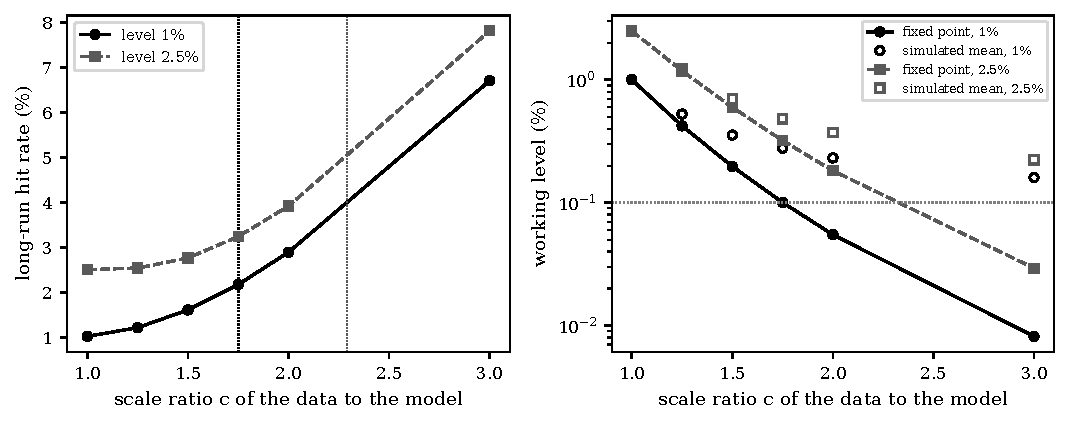
\includegraphics[width=\textwidth]{scale-sweep}
\caption{The wrapper facing a model that misjudges the scale of the data by a ratio $c$ (Student-$t$ with five degrees of freedom, 50 replications of 5,000 days): the long-run hit rate (left) and the fixed point and simulated mean of the working level on a logarithmic axis (right), at the 1\% and 2.5\% levels; the vertical dotted lines mark the largest repairable ratio of each level and the horizontal dotted line the lower edge of the band.}
\label{fig:scale-sweep}
\end{figure}

\subsection{The expected shortfall carried by the working level}
\label{sec:theory-es}

\begin{proposition}[ES at the fixed point of a Pareto tail]
\label{prop:es}
Let the model's tail be exactly a Pareto law of index $\xi < 1$, $V(a) = x_m a^{-\xi}$ and $E(a) = V(a)/(1-\xi)$, facing losses with the same tail shape and a scale $c$ times larger. At the fixed point $a^* = \alpha c^{-1/\xi}$ the wrapped ES equals the true ES at level $\alpha$.
\end{proposition}
\begin{proof}
The true VaR at level $\alpha$ is $c\,x_m\alpha^{-\xi}$ and the fixed point makes $x_m a^{*-\xi}$ equal to it, so $a^* = \alpha c^{-1/\xi}$. Then $E(a^*) = V(a^*)/(1-\xi) = c\,x_m\alpha^{-\xi}/(1-\xi)$, which is the true ES of the scaled law, $c\,E(\alpha)$.
\end{proof}

The Pareto tail is the case in which the ratio $r(a) = E(a)/V(a)$ does not depend on the level, and the proposition is that case: the wrapped ES is exact when the ratio is level-free. When it is not, the ratio of the wrapped ES to the true ES at the fixed point is $r(a^*)/r(\alpha)$. For the Student-$t$ law the ratio $r(a)$ rises with $a$ above its limit $\nu/(\nu-1)$ at $a \to 0$, and since $a^* < \alpha$ the wrapped ES is below the true one. The computation of \cref{sec:reproducibility} (Student-$t$ with 3, 5, 10 and 30 degrees of freedom at $c = 2$ and the 1\% level) gives a ratio of \thDRatioNuThree{}, \thDRatioNuFive{}, \thDRatioNuTen{} and \thDRatioNuThirty{}: an understatement of the ES by 2\% to 8\% that grows with the degrees of freedom, as the tail loses its power-law shape. The monotonicity of $r$ is checked on these four laws and on the two target levels and is not proved for all $\nu$.

\subsection{A conjecture on the score}
\label{sec:theory-conjecture}

\emph{Conjecture.} For a location-scale model with a scale error that the band allows to repair, the expected FZ0 score of the wrapped pair at the fixed point is lower than that of the unwrapped pair, by an amount that grows with $c$ and is largest for the models whose unwrapped ES is furthest from the truth. The evidence is of three kinds. The score of \cref{eq:fz0} is strictly consistent for the pair of the true VaR and ES, so any change that moves the VaR towards the true quantile lowers the expected score as long as the paired ES does not move away from the true ES by more than the VaR gains, and \cref{prop:es} shows that the wrapped ES moves to the true ES for a Pareto tail and stays within a few percent for the Student-$t$ tails. In the generators of known truth the median relative change of the score of the wrapped pair is negative for historical simulation in the three scenarios with a shift and at most \genFzPosMax\% for any model and scenario, which is inside the 5\% tolerance everywhere (\cref{tab:generators}). On the real windows the wrapped pair lowers the mean score in most of the cells, the worst change being \tenWorstFz\% (\cref{fig:fz0-change}). The conjecture is not proved: the condition on the paired ES is the part for which no argument is given, and a counter-example would be a model whose ES at the working level overstates the true ES by more than its VaR gains; the cells of the experiments with a positive change of the score (the filtered models in the generators) are of that kind.

\subsection{Conditions}
\label{sec:theory-conditions}

The statements hold under conditions that the experiments exercise. \Cref{prop:identity} holds for every run and every sequence, with the stated bound; it needs the update to be applied in time order with the hit of the day observed before the next day's level is used. \Cref{prop:independence} concerns the existence of a sequence, and needs $\gamma m(1-\alpha) < \alpha - \ell$ to avoid clipping. \Cref{prop:fixed-point} assumes independent and identically distributed standardised losses and a model that is a pure scale error of the truth; real windows have a changing volatility and a model that may be wrong in shape, so the proposition is a description of a limiting case that the generator experiments and the scale sweep test, not a theorem about the stress windows. \Cref{prop:es} assumes a Pareto tail for both the model and the truth. Two conditions bear on all four statements together. The hit of a day must be known before the level of the next day is used, so a delay in the confirmation of the hit shifts the update and is outside the identity as stated. The model must return a finite VaR and ES at every level of the band: the engine refuses a forecast that is not finite, and the experiments repeat the previous forecast on such a day and count it (\tenFallback{} days in all, in the \tenIndRunsAll{} wrapped runs of the six windows).

\section{Experimental design}
\label{sec:experimental-design}

\subsection{Hypotheses}
\label{sec:design-hypotheses}

The two statements below were written in the design document of the product before any wrapped run on a stress window, and are tested as written.

\begin{quote}
\textbf{H1.} HS-250, GARCH-t and FHS wrapped pass in at least one more stress window without worsening FZ0 by more than 5\%.\\
\textbf{H2 (refutation).} H1 is refuted if the wrapper fails independence in 2007--09.
\end{quote}

The terms are made exact by four conventions fixed with the hypotheses. A model \emph{passes} a window at a level when the Kupiec test and the conditional coverage test both have p-value at least 0.05; a test that the engine cannot evaluate (no hit in the window) passes nothing. The stress windows are the financial crisis window of 2007 to 2009, the pandemic window of 2020 and the rate-hiking window of 2022. H1 holds for a \emph{cell}, a model at a tail level (1\% or 2.5\%), when the wrapped model passes in at least one more of the three stress windows than the unwrapped one and its mean FZ0 is worse than that of the unwrapped model by at most 5\% in every stress window; it holds as a whole when it holds in all six cells and H2 does not occur. The wrapper \emph{fails independence} in a cell when the Christoffersen independence p-value of the wrapped model in the 2007--09 window is below 0.05. The step $\gamma = \gammaDefault$ and the band $[0.001, 0.25]$ were fixed before any run and were not tuned on any window.

Five further predictions follow from the theory and were written down before the generators of known truth were first run (they are listed in the header of the script \texttt{e5\_generators.py}): (a) in every scenario with a shift, for every model and level, the wrapped pass rate is above the unwrapped one; (b) with no shift the wrapped pass rate is within 0.05 of the unwrapped one and the median relative score change is within 2\%; (c) the wrapped mean hit rate is closer to the target in every scenario with a shift; (d) the repair is least complete in the shortest scenario, the decaying crash; (e) the wrapper lowers the mean absolute log error of the VaR against the true VaR for historical simulation in every scenario with a shift. The comparison with other recalibrations, the ablation and the extension from three models to ten were designed after the first results on the three models were known and carry no prediction.

\subsection{Data and its provenance}
\label{sec:design-data}

The data are three public daily series, taken as the case of Contraste takes them: the US equity market return from the Kenneth French data library (Mkt-RF plus RF), which is distributed for derived use only, so the returns are read from the device data root and only scores computed from them are committed; the ten-year US Treasury par yield from the Treasury's daily curve, converted to a return by the negative modified duration at the previous day's yield times the yield change; and the euro against the US dollar from the Federal Reserve's H.10 release. Six windows are built from them, with the portfolio of each window fixed in advance (\cref{tab:windows}): three stress windows (the first three rows), a foreign-exchange window of the financial crisis (251 days), a window of the bank turmoil of 2023 (64 days) and a calm control window of 2004 to 2006 (750 days). Equity returns are those of the market portfolio of the library; the mixed portfolios hold 50\% equity, 30\% rates and 20\% foreign exchange with daily rebalancing. A day on which any component is missing is skipped and counted, never filled. The hyperparameters of the models (the EWMA decay, the age-weighting decay, the threshold fraction of the extreme-value model) were selected once on the span 1995 to 2003, which ends before the earliest window, and are never changed. The factor library of \citet{fama1993} documents the construction of the equity series.

\begin{table*}[htbp]
\centering
\small
\caption{The six windows of case C11: the asset class of the portfolio, the first and last forecast day, the number of forecast days and of observed days of the common calendar, the public series of the portfolio and the role of the window in the evaluation.}
\label{tab:windows}
\begin{adjustbox}{max width=\textwidth}
\begin{tabular}{llllrrll}
\toprule
Window & Class & First forecast day & Last forecast day & Forecast days & Observed days & Series & Role \\
\midrule
Equity 2007--09 & equity & 2007-07-02 & 2009-06-30 & 504 & 1,504 & french--daily & stress \\
Equity 2020 & equity & 2020-02-03 & 2020-06-30 & 104 & 1,104 & french--daily & stress \\
Rates 2022 & rates & 2022-01-03 & 2022-12-30 & 249 & 1,249 & treasury--par & stress \\
FX 2008 & fx & 2008-07-01 & 2009-06-30 & 251 & 1,251 & h10--fx & other \\
Mixed 2023 & mixed & 2023-03-01 & 2023-05-31 & 64 & 1,064 & french--daily, treasury--par, h10--fx & other \\
Calm 2004--06 & mixed & 2004-01-02 & 2006-12-29 & 750 & 1,746 & french--daily, treasury--par, h10--fx & other \\
\bottomrule
\end{tabular}
\end{adjustbox}
\end{table*}


The three stress windows hold \hypStressDays{} forecast days in all (504, 104 and 249). The expected number of hits at the 1\% level is 5.0, 1.0 and 2.5 days, which is the reason the Kupiec test is read with its asymptotic caveat: its chi-square approximation is crude at counts this small, and the p-values of the engine are the asymptotic ones.

\subsection{Models compared, run by the product}
\label{sec:design-models}

The ladder holds eighteen models, all run by the pipeline of the product on the same windows with strictly rolling one-day forecasts that read only the returns before the forecast day: historical simulation over 250 and 500 days, the age-weighted variant, delta-normal and Cornish--Fisher with rolling moments, EWMA, GARCH, GJR-GARCH and EGARCH with Student-$t$ innovations, filtered historical simulation, the conditional extreme-value model, three CAViaR models (two for the VaR only, one with the ES step), three GAS-FZ models, and a quantile network trained on FZ0. Ten of them answer a VaR and an ES at any tail level and are wrapped: HS-250, HS-500, the age-weighted model, delta-normal, EWMA, GARCH-t, GJR-t, EGARCH-t, filtered historical simulation and the conditional extreme-value model. The Cornish--Fisher model and two CAViaR models give no ES, and the ES-CAViaR, the three GAS-FZ models and the network are fitted for one level and cannot be asked at another without a refit; they enter the ladder context and the score-space recalibrations but not the level wrapper.

Two recalibrations that act on the finished forecasts are run on the same forecasts as comparators. With the loss $L_t$ and the model's forecast $V_t$, define the score $S_t = L_t/V_t$, so that a hit is $S_t > 1$, and apply a scale $\theta_t$ to the VaR and the ES, $V_t^{\theta} = \theta_t V_t$ and $E_t^{\theta} = \theta_t E_t$.
The first is the rolling split-conformal scale: $\theta_t$ is the $k$-th smallest of the last $n \le \eqnRollWindow$ scores of the window with $k = \lceil (n+1)(1-\alpha)\rceil$, and 1 while $k > n$, clipped to $[0.25, 4]$ \citep{vovk2005,lei2018,barber2023}.
The second is the quantile tracker, the proportional term of conformal PID control \citep{angelopoulos2023}:
\begin{equation}
\theta_{t+1} = \max\bigl\{\theta_t + \eta\,(\indic\{S_t > \theta_t\} - \alpha),\ 0.25\bigr\}, \qquad \theta_1 = 1,
\label{eq:tracker}
\end{equation}
with $\eta = 0.05$ fixed before the run and $\eta \in \{0.01, 0.2\}$ reported as a sensitivity. Both are applied to all eighteen models; they need no model at another level.

\subsection{Metrics}
\label{sec:design-metrics}

For a sequence of $T$ forecast days with $x$ hits, the Kupiec test statistic is
\begin{equation}
\mathrm{LR}_{\mathrm{POF}} = -2\ln\frac{(1-\alpha)^{T-x}\alpha^{x}}{(1-x/T)^{T-x}(x/T)^{x}}, \label{eq:kupiec}
\end{equation}
asymptotically $\chi^2_1$ under the target frequency; the independence statistic $\mathrm{LR}_{\mathrm{ind}}$ is \cref{eq:lr-ind} computed with the observed transition counts of the sequence, asymptotically $\chi^2_1$, and the conditional coverage statistic is the sum $\mathrm{LR}_{\mathrm{POF}} + \mathrm{LR}_{\mathrm{ind}}$, asymptotically $\chi^2_2$ \citep{christoffersen1998,kupiec1995}. All three are computed by the engine and the p-values are the asymptotic ones. The score is the mean of \cref{eq:fz0} over the window, $\overline{\mathrm{FZ0}}$, and the change of a recalibration against the unwrapped model is
\begin{equation}
\Delta = \frac{\overline{\mathrm{FZ0}}_{\text{recalibrated}} - \overline{\mathrm{FZ0}}_{\text{unwrapped}}}{\bigl|\overline{\mathrm{FZ0}}_{\text{unwrapped}}\bigr|},
\label{eq:delta-fz0}
\end{equation}
positive when the recalibration scores worse, the quantity of the engine's \texttt{aci\_compare}. The ES is read through $Z_2$ of \cref{eq:z2}. The accuracy against a known truth, in the generators, is the mean absolute log error of the VaR against the true conditional VaR, $\frac{1}{T}\sum_t |\ln(V_t/V_t^{\mathrm{true}})|$, and its mean signed value as the bias. Four quantities describe the wrapper itself and are reported beside the tests: the hit rate $x/T$ with its Wilson interval, the mean working level, the number of days on which the band clipped the level, and the minimum of the path. The pass rate of a group of cells is the number of cells with a pass divided by the number of cells, so that it is a proportion over runs and carries a Wilson interval only where the runs are independent replications, as they are in the generators and are not in the real windows, where the cells share days.

\subsection{Protocol, statistics and planned ablations}
\label{sec:design-protocol}

On the real windows there is one realised path per window, so the uncertainty of a hit rate is its Wilson interval \citep{brown2001,wilson1927}, and the uncertainty of the change $\Delta$ is the 95\% percentile interval of a moving-block bootstrap with circular blocks of 10 days and 2,000 draws, which resamples the days of the paired daily scores jointly for the unwrapped and the recalibrated model \citep{kunsch1989,politis1994}. The seed of a draw is 20261104 plus a fixed integer per window, model and level. The bootstrap interval covers the variability of the score within the path and not the variability of the path itself, which one realised crisis cannot give; the generators supply the second kind. The generators of known truth use 100 replications per scenario, each with its own seed (the base 20261104 plus 1000 times the scenario index plus the replication), a design in the spirit of \citet{morris2019}: the pass rate of each method has its Wilson interval and the error against the truth its mean over replications.

The ablation changes one component of the wrapper at a time: the step ($\gamma \in \{0.001, 0.0025, 0.01, 0.02, 0.05\}$ against the default), the band (wider, $[10^{-5}, 0.5]$, and narrower, $[\alpha/2, 2\alpha]$) and the ES paired with the recalibrated VaR (the ES keeping the model's ratio to the VaR at the target level, and the ES left at the target level), on HS-250, GARCH-t and FHS at both levels in the three stress windows. The theory is checked by four numerical experiments (\cref{sec:reproducibility}): the identity of \cref{prop:identity} on the real level paths, the clustered sequence of \cref{prop:independence}, the scale sweep of \cref{prop:fixed-point} and the ES ratio of \cref{prop:es}. The unwrapped run of every model is checked against the forecasts of the ladder day by day, and the wrapped runs of the three models of H1 against the committed documents of the product; a mismatch stops the experiment.

\section{Results}
\label{sec:results}

\subsection{The three models of the prediction in the stress windows}
\label{sec:results-main}

\Cref{tab:main-results} gives, for HS-250, GARCH-t and filtered historical simulation, the hits of the unwrapped and the wrapped model in each stress window and level, the Kupiec and conditional coverage p-values, the independence p-value of the wrapped model and the change of the mean score with its bootstrap interval. The wrapped model has fewer hits than the unwrapped one in 16 of the 18 rows, and equal in the other two (FHS in the pandemic window at the 1\% level and in the rates window at 1\%, where the unwrapped model already passes). The largest reductions are those of historical simulation: in the financial crisis window the unwrapped model has \hitUHsTwoFiftyOneEqCrisis{} hits at the 1\% level against \hitWHsTwoFiftyOneEqCrisis{} wrapped, with \nDaysEqCrisis{} days expected to give 5.0, and at the 2.5\% level \hitUHsTwoFiftyTwoHalfEqCrisis{} against \hitWHsTwoFiftyTwoHalfEqCrisis{}. The Kupiec p-value of the wrapped historical simulation in that window is \kupWHsTwoFiftyOneEqCrisis{} at 1\%, below 0.05: the wrapped model still fails the unconditional test at the 1\% level, and it passes at 2.5\% (\kupWHsTwoFiftyTwoHalfEqCrisis{}, conditional coverage \ccWHsTwoFiftyTwoHalfEqCrisis{}). In the pandemic window, historical simulation stays below the bar at both levels after the wrap (Kupiec p-values \kupWHsTwoFiftyOneEqCovid{} and \kupWHsTwoFiftyTwoHalfEqCovid{}), with 6 and 7 hits in 104 days against 1.0 and 2.6 expected; the crash of March 2020 comes with the level already at the lower edge of the band (\clipHsTwoFiftyOneEqCovid{} days at the edge at the 1\% level).

\begin{table*}[htbp]
\centering
\small
\caption{Unwrapped (U) and wrapped (W) value at risk of three ladder models in the three stress windows of C11, at tail levels 1\% and 2.5\%: hits, the hit rate of the wrapped model with its 95\% Wilson interval, the p-values of the Kupiec and conditional coverage (CC) tests, the Christoffersen independence p-value of the wrapped model and the relative change of the mean FZ0 score with a 95\% moving-block bootstrap interval (positive is worse). The windows hold 504, 104 and 249 forecast days.}
\label{tab:main-results}
\begin{adjustbox}{max width=\textwidth}
\begin{tabular}{llrrlllll}
\toprule
Window & Model & Level (\%) & Hits U & Hits W (rate \%; 95\% Wilson) & Kupiec $p$ U / W & CC $p$ U / W & Indep. $p$ W & FZ0 change [95\% CI] \\
\midrule
Equity 2007--09 & HS-250 & 1 & 19 & 11 (2.2; 1.2--3.9) & $<0.001$ / 0.021 & $<0.001$ / 0.055 & 0.483 & \relax -17.2\% [-59.9\%, -1.3\%] \\
Equity 2007--09 & HS-250 & 2.5 & 36 & 17 (3.4; 2.1--5.3) & $<0.001$ / 0.233 & $<0.001$ / 0.271 & 0.275 & \relax -14.3\% [-40.3\%, -1.8\%] \\
Equity 2007--09 & GARCH-t & 1 & 16 & 6 (1.2; 0.5--2.6) & $<0.001$ / 0.677 & $<0.001$ / 0.853 & 0.703 & \relax -4.2\% [-12.4\%, +1.8\%] \\
Equity 2007--09 & GARCH-t & 2.5 & 31 & 14 (2.8; 1.7--4.6) & $<0.001$ / 0.695 & $<0.001$ / 0.620 & 0.371 & \relax -3.6\% [-10.5\%, +1.5\%] \\
Equity 2007--09 & FHS & 1 & 13 & 7 (1.4; 0.7--2.8) & 0.003 / 0.407 & 0.009 / 0.643 & 0.657 & \relax -3.2\% [-10.8\%, +1.7\%] \\
Equity 2007--09 & FHS & 2.5 & 24 & 14 (2.8; 1.7--4.6) & 0.004 / 0.695 & 0.005 / 0.620 & 0.371 & \relax -1.7\% [-6.5\%, +2.1\%] \\
Equity 2020 & HS-250 & 1 & 8 & 6 (5.8; 2.7--12.0) & $<0.001$ / 0.001 & $<0.001$ / 0.002 & 0.327 & \relax -168.7\% [-1274.5\%, +13.0\%] \\
Equity 2020 & HS-250 & 2.5 & 13 & 7 (6.7; 3.3--13.2) & $<0.001$ / 0.022 & $<0.001$ / 0.055 & 0.468 & \relax -631.7\% [-2271.3\%, +17.5\%] \\
Equity 2020 & GARCH-t & 1 & 3 & 2 (1.9; 0.5--6.7) & 0.116 / 0.401 & 0.265 / 0.676 & 0.778 & \relax +3.0\% [-3.4\%, +28.2\%] \\
Equity 2020 & GARCH-t & 2.5 & 6 & 5 (4.8; 2.1--10.8) & 0.067 / 0.180 & 0.116 / 0.185 & 0.209 & \relax -2.2\% [-24.6\%, +5.8\%] \\
Equity 2020 & FHS & 1 & 2 & 2 (1.9; 0.5--6.7) & 0.401 / 0.401 & 0.676 / 0.676 & 0.778 & \relax +3.4\% [+1.1\%, +10.3\%] \\
Equity 2020 & FHS & 2.5 & 5 & 4 (3.8; 1.5--9.5) & 0.180 / 0.415 & 0.316 / 0.610 & 0.570 & \relax +1.5\% [-0.2\%, +4.5\%] \\
Rates 2022 & HS-250 & 1 & 8 & 4 (1.6; 0.6--4.1) & 0.005 / 0.377 & 0.016 / 0.644 & 0.754 & \relax -5.8\% [-24.9\%, +3.5\%] \\
Rates 2022 & HS-250 & 2.5 & 14 & 8 (3.2; 1.6--6.2) & 0.007 / 0.490 & 0.011 / 0.624 & 0.495 & \relax -3.3\% [-10.5\%, +1.3\%] \\
Rates 2022 & GARCH-t & 1 & 6 & 4 (1.6; 0.6--4.1) & 0.058 / 0.377 & 0.147 / 0.644 & 0.754 & \relax -0.2\% [-7.5\%, +4.5\%] \\
Rates 2022 & GARCH-t & 2.5 & 14 & 8 (3.2; 1.6--6.2) & 0.007 / 0.490 & 0.011 / 0.624 & 0.495 & \relax -0.3\% [-3.0\%, +1.6\%] \\
Rates 2022 & FHS & 1 & 5 & 5 (2.0; 0.9--4.6) & 0.160 / 0.160 & 0.343 / 0.343 & 0.685 & \relax +0.9\% [-3.4\%, +3.9\%] \\
Rates 2022 & FHS & 2.5 & 12 & 7 (2.8; 1.4--5.7) & 0.037 / 0.758 & 0.065 / 0.801 & 0.555 & \relax -0.3\% [-3.0\%, +1.4\%] \\
\bottomrule
\end{tabular}
\end{adjustbox}
\end{table*}


\Cref{fig:hit-rates} shows the same results as hit rates with their Wilson intervals: the wrapped hit rate is closer to the target than the unwrapped one, or equal to it, in every cell. The intervals are wide, because the windows hold between 2 and 36 hits in each cell of the unwrapped models and between 2 and 17 in the wrapped ones: the interval of the wrapped hit rate of GARCH-t at the 1\% level in the crisis window is 0.5\% to 2.6\%, which contains the target. \Cref{fig:level-paths} shows what the wrapper did. The working level of historical simulation falls to the band edge on \clipHsTwoFiftyOneEqCrisis{} days of the crisis window and on \clipHsTwoFiftyOneRates{} days of the rates window at the 1\% level and recovers slowly between clusters, as \cref{eq:cluster-drop} predicts: a single hit at the 1\% level needs about 100 quiet days to be undone. The level of GARCH-t, whose own volatility filter follows the crisis, reaches the edge on \clipGarchTOneEqCrisis{} days in the crisis window and on none in the pandemic window, where its minimum level is 0.0045.

\begin{figure}[htbp]
\centering
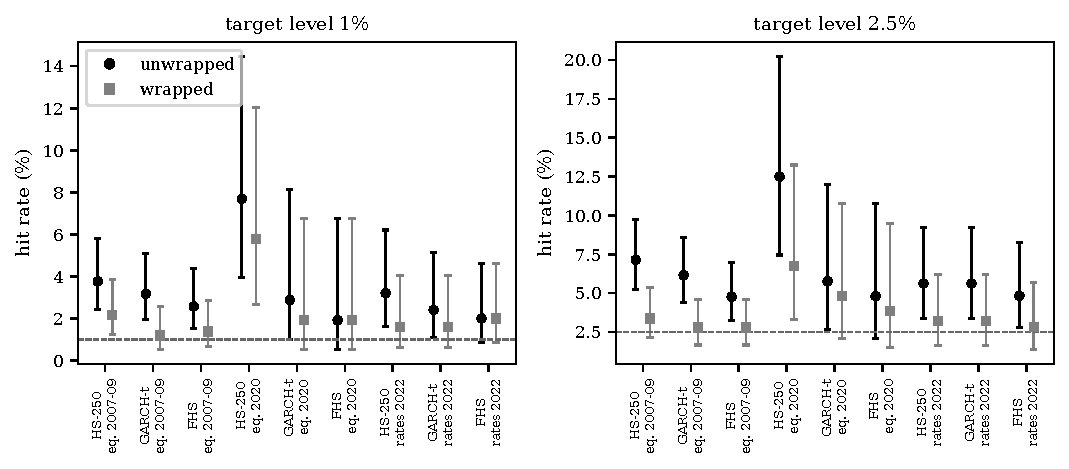
\includegraphics[width=\textwidth]{hit-rates}
\caption{Hit rate of the unwrapped (circles) and wrapped (squares) value at risk of HS-250, GARCH-t and FHS in the three stress windows, at the 1\% (left) and 2.5\% (right) target levels, with 95\% Wilson intervals; the dashed line is the target.}
\label{fig:hit-rates}
\end{figure}

\begin{figure}[htbp]
\centering
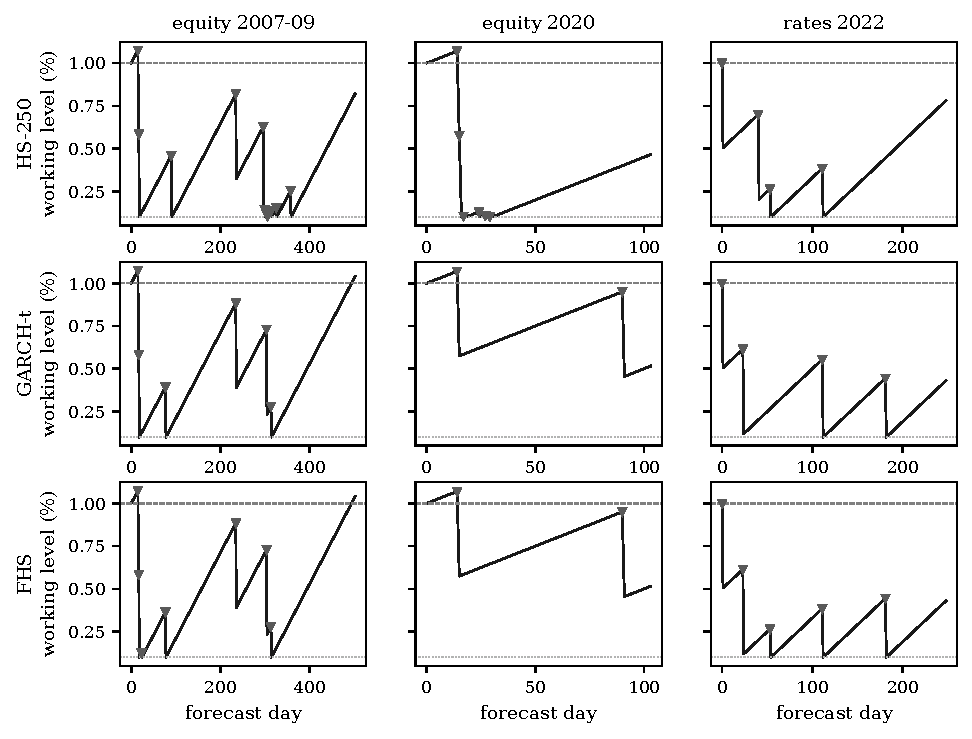
\includegraphics[width=\textwidth]{level-paths}
\caption{Working level of the wrapper at the 1\% target for HS-250, GARCH-t and FHS (rows) in the three stress windows (columns): the level in percent by forecast day, the days of a hit of the wrapped model marked by triangles, the target as a dashed line and the lower edge of the band as a dotted line.}
\label{fig:level-paths}
\end{figure}

\subsection{Whether the hypotheses held}
\label{sec:results-hypotheses}

\Cref{tab:hypotheses} applies the rule of H1 to the six cells of the hypothesis and to the other fourteen cells of the ten wrapped models. H1 holds in all \hypCells{} cells of HS-250, GARCH-t and FHS: the wrapped models gain \hypExtraTotal{} stress-window passes in all (HS-250 one window at 1\% and two at 2.5\%, GARCH-t one and two, FHS one and two), and the worst change of the mean score in any stress window is \hypWorstFz\%, below the 5\% tolerance. H2 does not occur: the independence p-values of the wrapped models in the crisis window run from \indMin{} to \indMax{}, and \indFails{} of the six are below 0.05. The hypothesis holds as a whole as it was written, with the engine's Kupiec and conditional coverage tests as the pass rule. Those tests accept wrapped runs more easily than unwrapped ones (\cref{sec:results-dispersion}); tested on coverage alone against the null of the wrapped count, H1 holds in \dispCHoneGainCal{} of the \hypCells{} cells, the cell that falls being \dispCHoneLost. The statement carries a qualification that the table makes visible: of the \hypExtraTotal{} extra passes, none comes from the pandemic window for HS-250, and the extra passes of GARCH-t and FHS are in the crisis window (and in the rates window at the 2.5\% level), where the unwrapped Kupiec p-values are 0.004 or below in the crisis window and at most 0.037 in the rates window.

Applied to the ten models, the rule holds in \tenCellsHold{} of \tenCells{} cells. The cell that fails is \tenNoGainCells{}: it gains no window, although its hit rate improves, and the level sits at the band edge on \clipDnRollingOneEqCrisis{} days of the crisis window, so the band, not the update, limits what the model can reach. Across the ten models the wrapped runs pass \tenPassAci{} of \tenRuns{} cells against \tenPassUnw{} unwrapped by the engine's tests (\dispCWrapCal{} against \dispCUnwExact{} on coverage alone, with each count tested against its own null; \cref{sec:results-dispersion}), no wrapped run fails the independence test in the stress windows (and none in the \tenIndRunsAll{} runs of all six windows), and the mean absolute distance of the hit rate from its target falls from \tenHitDevUnw{} to \tenHitDevAci{} percentage points.

\begin{table}[htbp]
\centering
\small
\caption{The prediction for each of the ten wrapped ladder models and two tail levels: windows passed (Kupiec and conditional coverage both at least 0.05) out of the three stress windows, unwrapped (U) and wrapped (W), the extra windows gained, the worst relative FZ0 change in any stress window, the independence p-value of the wrapped model in equity 2007--09 and whether the prediction holds. The first six rows are the models of the prediction as stated; the other rows apply the same rule to the remaining models.}
\label{tab:hypotheses}
\begin{adjustbox}{max width=\textwidth}
\begin{tabular}{lrrrrrrl}
\toprule
Model & Level (\%) & Windows passed U & Windows passed W & Extra & Worst FZ0 change & Indep. $p$ W, 2007--09 & Holds \\
\midrule
HS-250 & 1 & 0 & 1 & 1 & \relax -5.8\% & 0.483 & yes \\
HS-250 & 2.5 & 0 & 2 & 2 & \relax -3.3\% & 0.275 & yes \\
HS-500 & 1 & 0 & 1 & 1 & \relax -0.9\% & 0.483 & yes \\
HS-500 & 2.5 & 0 & 2 & 2 & \relax -5.0\% & 0.248 & yes \\
AWHS & 1 & 0 & 1 & 1 & \relax -1.1\% & 0.483 & yes \\
AWHS & 2.5 & 1 & 3 & 2 & \relax -0.4\% & 0.305 & yes \\
Delta-normal & 1 & 0 & 0 & 0 & \relax -21.9\% & 0.935 & no \\
Delta-normal & 2.5 & 0 & 1 & 1 & \relax -10.0\% & 0.836 & yes \\
EWMA & 1 & 1 & 2 & 1 & \relax -0.0\% & 0.657 & yes \\
EWMA & 2.5 & 1 & 2 & 1 & \relax +0.3\% & 0.371 & yes \\
GARCH-t & 1 & 2 & 3 & 1 & \relax +3.0\% & 0.703 & yes \\
GARCH-t & 2.5 & 1 & 3 & 2 & \relax -0.3\% & 0.371 & yes \\
GJR-t & 1 & 2 & 3 & 1 & \relax +2.9\% & 0.703 & yes \\
GJR-t & 2.5 & 1 & 3 & 2 & \relax -0.9\% & 0.337 & yes \\
EGARCH-t & 1 & 2 & 3 & 1 & \relax -0.2\% & 0.567 & yes \\
EGARCH-t & 2.5 & 0 & 3 & 3 & \relax -0.8\% & 0.248 & yes \\
FHS & 1 & 2 & 3 & 1 & \relax +3.4\% & 0.657 & yes \\
FHS & 2.5 & 1 & 3 & 2 & \relax +1.5\% & 0.371 & yes \\
Conditional EVT & 1 & 2 & 3 & 1 & \relax +4.3\% & 0.703 & yes \\
Conditional EVT & 2.5 & 1 & 3 & 2 & \relax +1.9\% & 0.371 & yes \\
\bottomrule
\end{tabular}
\end{adjustbox}
\end{table}


\subsection{The score of the pair}
\label{sec:results-score}

The change of the mean score is the second condition of H1, and \cref{fig:fz0-change} shows it for the ten models with the bootstrap intervals. The change is negative (the wrapped pair scores better) in most cells, with a mean of \tenMeanFz\% over the \tenRuns{} cells, and the largest improvement is that of HS-500 at the 2.5\% level in the pandemic window (\tenBestFz\%), where the unwrapped VaR sits near the calm past on a sudden crash. The largest positive changes are those of the filtered models and the extreme-value model at the 1\% level (\worstFzGarchTOne\% for GARCH-t, \worstFzFhsOne\% for FHS, \worstFzEvtMfOne\% for the extreme-value model), all below the 5\% tolerance, and their intervals contain zero in most windows (\cref{fig:fz0-change}); the one exception in the table is FHS in the pandemic window at the 1\% level, with an interval of +1.1\% to +10.3\%, whose upper end is over the tolerance. The intervals of the historical-simulation cells in the pandemic window run from $-1{,}274.5\%$ to $+13.0\%$ at the 1\% level and from $-2{,}271.3\%$ to $+17.5\%$ at 2.5\% (\cref{tab:main-results}) because the unwrapped score is close to zero on 104 days and its relative change is unstable; the absolute differences are the better guide there.

\begin{figure}[htbp]
\centering
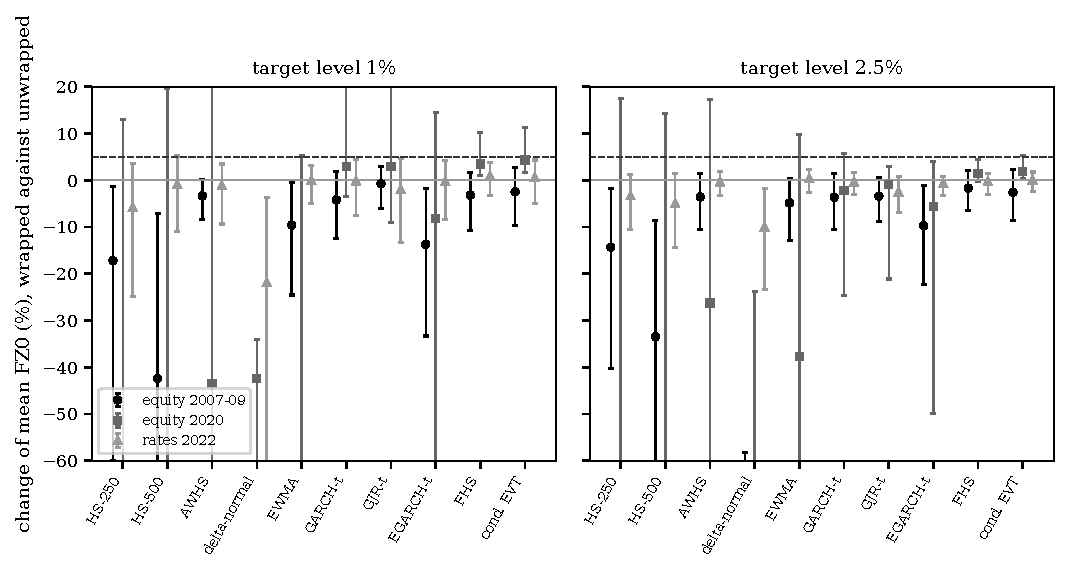
\includegraphics[width=\textwidth]{fz0-change}
\caption{Relative change of the mean FZ0 score of the wrapped against the unwrapped model for the ten wrapped ladder models in the three stress windows, at the 1\% (left) and 2.5\% (right) levels, with 95\% moving-block bootstrap intervals; the dashed line is the 5\% tolerance and values below zero are improvements.}
\label{fig:fz0-change}
\end{figure}

The ES stays understated: the mean $Z_2$ of the ten models in the stress windows is \tenMeanZtwoUnw{} unwrapped and \tenMeanZtwoAci{} wrapped, a halving of the shortfall that leaves it far from zero. The wrapper repairs the VaR and carries the ES along, but it does not make the ES correct, which is the content of \cref{prop:es} for tails that are not Pareto.

\subsection{The ladder as a whole}
\label{sec:results-ladder}

\Cref{tab:ladder-context} and \cref{fig:ladder-pass} put the wrapped models back among the eighteen. In the crisis window no model of the ladder passes at either level as the ladder runs. With the three models of H1 replaced by their wrapped versions, \ladThreeEqCrisisOne{} pass at the 1\% level and \ladThreeEqCrisisTwoHalf{} at 2.5\%; with the ten wrapped models, \ladTenEqCrisisOne{} and \ladTenEqCrisisTwoHalf{} of the eighteen. In the pandemic window the count rises from \ladUEqCovidOne{} to \ladTenEqCovidOne{} at 1\% and from \ladUEqCovidTwoHalf{} to \ladTenEqCovidTwoHalf{} at 2.5\%; in the rates window from \ladURatesOne{} to \ladTenRatesOne{} and from \ladURatesTwoHalf{} to \ladTenRatesTwoHalf{}. The eight models that are not wrapped (three that give no ES, five fitted for one level) keep their unwrapped results in these counts, so the figures understate what a wrap of every model would give. The counts of the wrapped models are the engine's, and inherit the lenience measured in \cref{sec:results-dispersion}: they show how many models the supervisor's tests would pass, not how many are correctly sized.

\begin{table}[htbp]
\centering
\small
\caption{The eighteen-model ladder of C11 in the three stress windows: how many models pass the Kupiec and conditional coverage tests (both p at least 0.05) as the ladder runs, with the three models of the prediction replaced by their wrapped versions, and with the ten level-parametric models replaced by their wrapped versions.}
\label{tab:ladder-context}
\begin{adjustbox}{max width=\textwidth}
\begin{tabular}{lrrrrr}
\toprule
Window & Level (\%) & Ladder models & Pass, none wrapped & Pass, three wrapped & Pass, ten wrapped \\
\midrule
Equity 2007--09 & 1 & 18 & 0 & 2 & 6 \\
Equity 2007--09 & 2.5 & 18 & 0 & 3 & 9 \\
Equity 2020 & 1 & 18 & 5 & 5 & 5 \\
Equity 2020 & 2.5 & 18 & 6 & 6 & 8 \\
Rates 2022 & 1 & 18 & 10 & 11 & 13 \\
Rates 2022 & 2.5 & 18 & 5 & 8 & 13 \\
\bottomrule
\end{tabular}
\end{adjustbox}
\end{table}


\begin{figure}[htbp]
\centering
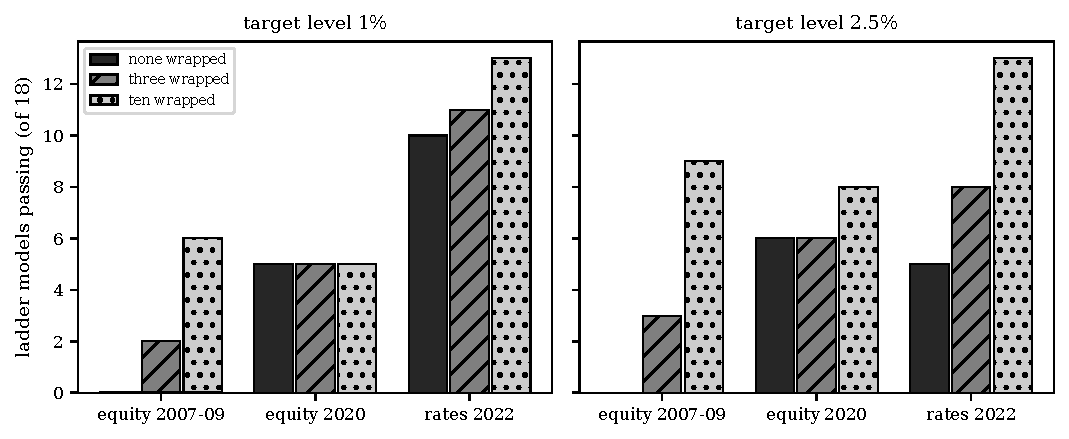
\includegraphics[width=\textwidth]{ladder-pass}
\caption{Number of the eighteen ladder models that pass the Kupiec and conditional coverage tests in each stress window at the 1\% (left) and 2.5\% (right) levels: as the ladder runs (dark bars), with the three models of the hypothesis wrapped (hatched bars) and with the ten level-parametric models wrapped (light bars).}
\label{fig:ladder-pass}
\end{figure}

\subsection{Against other recalibrations}
\label{sec:results-comparators}

\Cref{tab:comparators} and \cref{fig:methods-pass} compare the wrapper with the two recalibrations that act on the finished VaR, run on the same VaR and the same ES (both scaled by the same factor) of the same ten models, so that the unwrapped baseline is the same for all of them. The wrapper passes \tenPassAci{} of \tenRuns{} cells, the rolling split-conformal scale \cmpRollTenPass{}, and the quantile tracker \cmpTrkTenPass{} at its pre-set step of 0.05, \cmpTrkSmallTenPass{} at 0.01 and \cmpTrkLargeTenPass{} at 0.2. The rolling scale ties the wrapper on passes but its mean score change is \cmpRollTenFz\% against \tenMeanFz\% for the wrapper: it breaks the score tolerance in \cmpRollTenFzOver{} of its \cmpRollTenFzN{} cells (worst change \cmpRollTenFzWorst\%, \cmpRollWorstModel{} at the \cmpRollWorstLevel\% level in \cmpRollWorstWin, where the unwrapped mean score is \cmpRollWorstBase{} and the scale reaches \cmpRollWorstScaleMax{} on a crash) and fails the independence test in \cmpRollTenInd{} cells. The tracker at 0.05 has no cell over the tolerance and passes fewer cells than the wrapper; the tracker at 0.2 passes the most cells, \cmpTrkLargeTenPass{}, and has the smallest distance of the hit rate from the target (\cmpTrkLargeTenDev{} points against \tenHitDevAci{} for the wrapper), at the price of \cmpTrkLargeTenFzOver{} cell over the score tolerance (worst change \cmpTrkLargeTenFzWorst\%). Applied to all eighteen ladder models, the rolling scale passes \cmpRollAllPass{} of \cmpRollAllN{} cells, the tracker \cmpTrkAllPass{} and the unwrapped ladder \cmpUnwAllPass{}. The pass counts of all these rows come from the same tests, and the rolling scale and the tracker also hold the hit count near its target (\cref{sec:results-dispersion}); the counts compare the rows with one another and with the unwrapped models only loosely.

The finding is not that the level wrapper beats the other recalibrations. On the number of cells passed it is tied with one, behind another at a larger step, and ahead of the tracker at its pre-set step. On the score it has no cell over the tolerance, as the tracker at 0.01 and 0.05 has, and it passes more cells than either of them; the rolling scale is as good on passes and worse on the score, and the tracker at the larger step is better on passes and on the hit rate and has \cmpTrkLargeTenFzOver{} cell over the tolerance. The result is specific to the pre-set constants: the step of the tracker is a free parameter, and the table shows that a larger step buys passes at a cost in the score that the step of the wrapper shows as well: in the ablation, steps above the default gain no cells and break the tolerance (\cref{sec:ablation}).

\begin{table}[htbp]
\centering
\small
\caption{Online recalibrations compared on the same forecasts: the ten level-parametric ladder models at two tail levels in the three stress windows (60 cells). A cell passes when the Kupiec and conditional coverage p-values are both at least 0.05; independence failures count the cells with a Christoffersen independence p-value below 0.05; the FZ0 change is relative to the unwrapped model.}
\label{tab:comparators}
\begin{adjustbox}{max width=\textwidth}
\begin{tabular}{lrrrrrr}
\toprule
Recalibration & Cells passing & Independence failures & Mean $|$hit $-$ target$|$ (points) & Mean FZ0 change & Worst FZ0 change & Cells over $+5\%$ \\
\midrule
Unwrapped & 17 / 60 & 2 & 4.02 & -- & -- & -- \\
\relax Level wrapper, $\gamma = 0.005$ (proposed) & 45 / 60 & 0 & 1.83 & \relax -45.7\% & \relax +4.3\% & 0 \\
Rolling split-conformal scale & 45 / 60 & 2 & 2.09 & \relax +0.4\% & \relax +353.6\% & 10 \\
\relax Quantile tracker, $\eta = 0.01$ & 23 / 60 & 0 & 3.26 & \relax -13.6\% & \relax +0.3\% & 0 \\
\relax Quantile tracker, $\eta = 0.05$ & 41 / 60 & 0 & 2.17 & \relax -35.4\% & \relax +1.3\% & 0 \\
\relax Quantile tracker, $\eta = 0.2$ & 52 / 60 & 0 & 1.11 & \relax -56.7\% & \relax +5.4\% & 1 \\
\bottomrule
\end{tabular}
\end{adjustbox}
\end{table}


\begin{figure}[htbp]
\centering
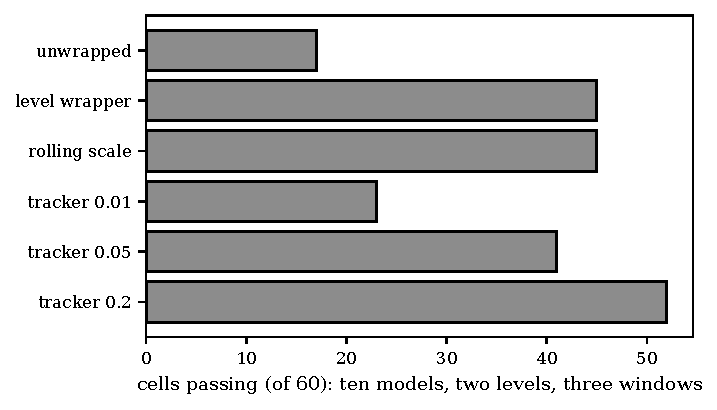
\includegraphics[width=0.62\textwidth]{methods-pass}
\caption{Cells passed (Kupiec and conditional coverage both at least 0.05) out of 60 by the unwrapped models, the level wrapper and four recalibrations of the finished value at risk, for the ten wrapped ladder models at two levels in the three stress windows.}
\label{fig:methods-pass}
\end{figure}

\subsection{Generators of known truth}
\label{sec:results-generators}

\Cref{tab:generators} and \cref{fig:generator-pass} give the generator study, with \genReps{} replications of each of four scenarios. With a shift, the wrapped pass rate is above the unwrapped one in all \genPredANum{} of \genPredADen{} model-level-scenario cells (prediction (a) held on the pass rates; \cref{sec:results-dispersion} shows how much of these differences the tests themselves produce). The unwrapped historical simulation passes in \genPassCrisisHsTwoFiftyOneUnw{} of replications of the persistent crisis at the 1\% level and the wrapped model in \genPassCrisisHsTwoFiftyOneAci{}; in the decaying crash the wrapped pass rate is \genPassCrashHsTwoFiftyOneAci{} for historical simulation at 1\%, the lowest of any shift cell (\genLowestAciPass{}, in \genLowestAciScen{}), which is prediction (d): the shortest window is repaired least. Prediction (c) held in \genPredCNum{} of the 18 cells with a shift, and (e) in \genPredENum{} of \genPredEDen{}: the wrapper lowers the mean error of the historical-simulation VaR against the true VaR in every scenario with a shift.

One prediction did not hold as stated. Prediction (b), that with no shift the wrapped pass rate is within 0.05 of the unwrapped one, held in \genPredBWithin{} of 6 cells: the wrapped pass rate is higher by \genPredBDiffMin{} to \genPredBDiffMax{}. The cause is not a mean hit rate off the target in the no-shift scenario: GARCH-t and FHS at the 1\% level have unwrapped mean hit rates of \genHitNullGarchTOneUnw\% and \genHitNullFhsOneUnw\%, on the target, and their pass rate still rises to \genPassNullGarchTOneAci{} and \genPassNullFhsOneAci{} once wrapped. Two properties of the counts raise it: the wrapped hit count is less variable than a binomial count and the tests accept it more easily, and the unwrapped counts of these two models are more variable than a binomial count, which lowers their own pass rate (\cref{sec:results-dispersion}); the mis-sizing of historical simulation at 1\% (a mean hit rate of \genHitNullHsTwoFiftyOneUnw\% in the control, a finite-sample understatement of the tail) is a second, partial cause for that model only. The second part of (b), a median score change within 2\%, held (largest \genPredBFzMax\%). A further negative result, which no prediction covered, concerns accuracy against the truth. For the two filtered models the wrapper raises the mean absolute log error of the VaR against the true VaR in \genErrWorseCells{} of \genErrWorseDen{} cells (four scenarios, two models, two levels): the fluctuation of the level adds noise to a VaR that the filter already tracks, so passes are gained at the price of VaR accuracy. The independence of the hits is not harmed in any generator cell: the share of replications with an independence p-value of at least 0.05 falls by at most \genIndDropMax{} (\cref{tab:generators}), a statement that carries the limit of the independence test discussed in \cref{sec:discussion-why}.

\begin{table*}[htbp]
\centering
\small
\caption{Generators of known truth, 100 replications per scenario: pass rate (Kupiec and conditional coverage both at least 0.05) of the unwrapped model and of three recalibrations, each with its 95\% Wilson interval; the mean absolute log error of the VaR against the true conditional VaR, unwrapped (U) and wrapped (W); and the median relative FZ0 change of the level wrapper.}
\label{tab:generators}
\begin{adjustbox}{max width=\textwidth}
\begin{tabular}{llrlllllr}
\toprule
Scenario & Model & Level (\%) & Unwrapped & Level wrapper & Rolling scale & Tracker & VaR error U / W & Median FZ0 change W \\
\midrule
No shift & HS-250 & 1 & 0.85 (0.77--0.91) & 0.99 (0.95--1.00) & 0.95 (0.89--0.98) & 0.93 (0.86--0.97) & 0.259 / 0.265 & \relax +0.2\% \\
No shift & HS-250 & 2.5 & 0.76 (0.67--0.83) & 0.94 (0.88--0.97) & 0.91 (0.84--0.95) & 0.91 (0.84--0.95) & 0.238 / 0.241 & \relax +0.1\% \\
No shift & GARCH-t & 1 & 0.85 (0.77--0.91) & 0.99 (0.95--1.00) & 0.99 (0.95--1.00) & 0.98 (0.93--0.99) & 0.051 / 0.107 & \relax +0.8\% \\
No shift & GARCH-t & 2.5 & 0.94 (0.88--0.97) & 1.00 (0.96--1.00) & 1.00 (0.96--1.00) & 1.00 (0.96--1.00) & 0.044 / 0.080 & \relax +0.4\% \\
No shift & FHS & 1 & 0.76 (0.67--0.83) & 0.99 (0.95--1.00) & 0.97 (0.92--0.99) & 0.92 (0.85--0.96) & 0.075 / 0.117 & \relax +0.6\% \\
No shift & FHS & 2.5 & 0.86 (0.78--0.91) & 1.00 (0.96--1.00) & 1.00 (0.96--1.00) & 1.00 (0.96--1.00) & 0.060 / 0.086 & \relax +0.4\% \\
Persistent crisis & HS-250 & 1 & 0.25 (0.18--0.34) & 0.92 (0.85--0.96) & 0.77 (0.68--0.84) & 0.73 (0.64--0.81) & 0.504 / 0.466 & \relax -9.4\% \\
Persistent crisis & HS-250 & 2.5 & 0.22 (0.15--0.31) & 0.96 (0.90--0.98) & 0.79 (0.70--0.86) & 0.80 (0.71--0.87) & 0.495 / 0.465 & \relax -6.5\% \\
Persistent crisis & GARCH-t & 1 & 0.62 (0.52--0.71) & 0.95 (0.89--0.98) & 0.97 (0.92--0.99) & 0.83 (0.74--0.89) & 0.177 / 0.166 & \relax +0.4\% \\
Persistent crisis & GARCH-t & 2.5 & 0.46 (0.37--0.56) & 0.99 (0.95--1.00) & 0.96 (0.90--0.98) & 0.92 (0.85--0.96) & 0.173 / 0.153 & \relax -0.1\% \\
Persistent crisis & FHS & 1 & 0.62 (0.52--0.71) & 0.95 (0.89--0.98) & 0.96 (0.90--0.98) & 0.84 (0.76--0.90) & 0.175 / 0.175 & \relax +0.8\% \\
Persistent crisis & FHS & 2.5 & 0.45 (0.36--0.55) & 0.99 (0.95--1.00) & 0.96 (0.90--0.98) & 0.94 (0.88--0.97) & 0.172 / 0.155 & \relax +0.2\% \\
Decaying crash & HS-250 & 1 & 0.26 (0.18--0.35) & 0.68 (0.58--0.76) & 0.26 (0.18--0.35) & 0.34 (0.25--0.44) & 0.460 / 0.451 & \relax -27.8\% \\
Decaying crash & HS-250 & 2.5 & 0.24 (0.17--0.33) & 0.81 (0.72--0.87) & 0.44 (0.35--0.54) & 0.39 (0.30--0.49) & 0.497 / 0.470 & \relax -14.1\% \\
Decaying crash & GARCH-t & 1 & 0.72 (0.63--0.80) & 0.93 (0.86--0.97) & 0.73 (0.64--0.81) & 0.78 (0.69--0.85) & 0.187 / 0.238 & \relax +1.9\% \\
Decaying crash & GARCH-t & 2.5 & 0.77 (0.68--0.84) & 0.96 (0.90--0.98) & 0.95 (0.89--0.98) & 0.90 (0.83--0.94) & 0.180 / 0.199 & \relax +0.1\% \\
Decaying crash & FHS & 1 & 0.70 (0.60--0.78) & 0.91 (0.84--0.95) & 0.72 (0.63--0.80) & 0.76 (0.67--0.83) & 0.198 / 0.243 & \relax +1.4\% \\
Decaying crash & FHS & 2.5 & 0.81 (0.72--0.87) & 0.98 (0.93--0.99) & 0.95 (0.89--0.98) & 0.94 (0.88--0.97) & 0.188 / 0.204 & \relax +0.1\% \\
Upward drift & HS-250 & 1 & 0.59 (0.49--0.68) & 0.97 (0.92--0.99) & 0.96 (0.90--0.98) & 0.77 (0.68--0.84) & 0.275 / 0.244 & \relax -2.2\% \\
Upward drift & HS-250 & 2.5 & 0.43 (0.34--0.53) & 0.95 (0.89--0.98) & 0.91 (0.84--0.95) & 0.66 (0.56--0.75) & 0.266 / 0.224 & \relax -1.4\% \\
Upward drift & GARCH-t & 1 & 0.87 (0.79--0.92) & 1.00 (0.96--1.00) & 0.98 (0.93--0.99) & 0.97 (0.92--0.99) & 0.117 / 0.131 & \relax +1.1\% \\
Upward drift & GARCH-t & 2.5 & 0.81 (0.72--0.87) & 1.00 (0.96--1.00) & 0.97 (0.92--0.99) & 0.98 (0.93--0.99) & 0.112 / 0.110 & \relax +0.3\% \\
Upward drift & FHS & 1 & 0.83 (0.74--0.89) & 0.99 (0.95--1.00) & 0.98 (0.93--0.99) & 0.93 (0.86--0.97) & 0.121 / 0.142 & \relax +0.8\% \\
Upward drift & FHS & 2.5 & 0.82 (0.73--0.88) & 0.99 (0.95--1.00) & 0.97 (0.92--0.99) & 0.96 (0.90--0.98) & 0.115 / 0.117 & \relax +0.4\% \\
\bottomrule
\end{tabular}
\end{adjustbox}
\end{table*}


\begin{figure}[htbp]
\centering
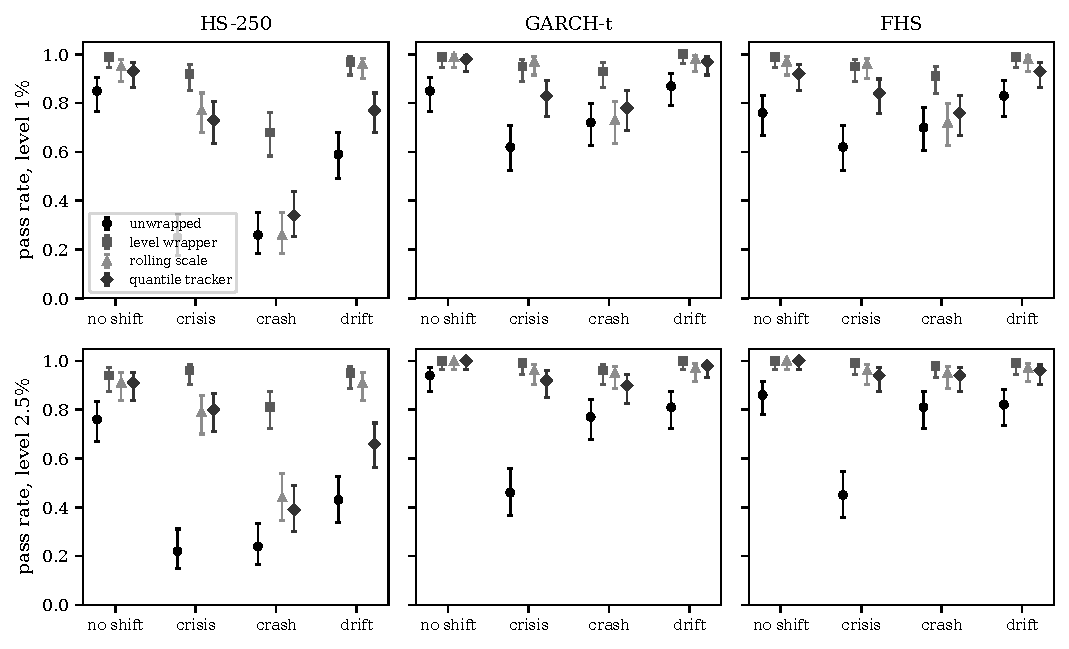
\includegraphics[width=\textwidth]{generator-pass}
\caption{Pass rate over 100 replications of each scenario for HS-250, GARCH-t and FHS at the 1\% (top) and 2.5\% (bottom) levels: the unwrapped model and three recalibrations, with 95\% Wilson intervals; the scenarios are no shift, a persistent crisis, a decaying crash and an upward drift of the volatility.}
\label{fig:generator-pass}
\end{figure}

\subsection{How easily the back-tests accept a wrapped run}
\label{sec:results-dispersion}

The no-shift scenario of the generators holds a result that the pass counts above cannot show. For GARCH-t and FHS at the 1\% level the unwrapped mean hit rate is \genHitNullGarchTOneUnw\% and \genHitNullFhsOneUnw\%, on the target, and the models pass in \genPassNullGarchTOneUnw{} and \genPassNullFhsOneUnw{} of the replications; the wrapped models pass in \genPassNullGarchTOneAci{} and \genPassNullFhsOneAci{} (\cref{tab:dispersion-null}). A mean on the target does not make these models right in each replication: the standard deviation of the unwrapped hit rate across replications is \dispSdNullGarchTOneUnw{} points for GARCH-t and \dispSdNullFhsOneUnw{} for FHS, against the binomial value of \dispBinNullGarchTOneUnw{} and \dispBinNullFhsOneUnw{} points for independent hits at that rate and that length (ratios \dispRatioNullGarchTOneUnw{} and \dispRatioNullFhsOneUnw{}), the estimation error of each replication, and their pass rates sit below the \dispBOneOneUnwPass\% of a model known to be correct (\cref{tab:dispersion}, $c = 1$). Part of the rise in the pass rate is therefore a repair of the coverage of each run, which the wrapper makes. The rest is the spread of the wrapped hit rate: its standard deviation falls to \dispSdNullGarchTOneAci{} points for GARCH-t and \dispSdNullFhsOneAci{} for FHS, below the binomial value. The wrapped hit count is under-dispersed. In the \dispRatioAciN{} model-level-scenario cells of the generators the ratio of the wrapped standard deviation to the binomial one runs from \dispRatioAciMin{} to \dispRatioAciMax{} (below one in \dispRatioAciBelow{} cells), for the rolling scale from \dispRatioRollMin{} to \dispRatioRollMax{} and for the quantile tracker from \dispRatioTrkMin{} to \dispRatioTrkMax{}, while for the unwrapped models it runs from \dispRatioUnwMin{} to \dispRatioUnwMax{}. This is the identity of \cref{prop:identity} at work: a hit lowers the level and a quiet day raises it, so the running count cannot wander far from its target, and the count is less variable than that of independent hits. The Kupiec and conditional coverage tests, and the Wilson interval of the hit rate, are built for independent hits; they accept a run whose count is held near the target more easily than its coverage warrants. In the no-shift scenario the pass rate of the wrapped models runs from \dispNullPassAciMin{} to \dispNullPassAciMax{}, that of the rolling scale from \dispNullPassRollMin{} to \dispNullPassRollMax{} and that of the tracker from \dispNullPassTrkMin{} to \dispNullPassTrkMax{}, against \dispNullPassUnwMin{} to \dispNullPassUnwMax{} for the unwrapped models. These ranges are not a measure of the size of the tests: the models of the scenario are estimated, not known, and HS-250 at the 2.5\% level has an unwrapped hit rate of \genHitNullHsTwoFiftyTwoHalfUnw\% against the target of 2.5\%. The size is measured next, on a model that is correct by construction.

\begin{table}[htbp]
\centering
\small
\caption{The control scenario (no shift, 500 days, 100 replications): the mean hit rate, the standard deviation of the hit rate across replications of the unwrapped (U) and wrapped (W) model against the binomial standard deviation at the unwrapped mean rate, and the pass rate of the unwrapped model and of three recalibrations.}
\label{tab:dispersion-null}
\begin{adjustbox}{max width=\textwidth}
\begin{tabular}{llrrr}
\toprule
Model & Level (\%) & Mean hit rate (\%) U / W & Hit-rate s.d. (points) U / W / binomial & Pass rate U / W / rolling / tracker \\
\midrule
HS-250 & 1 & 1.31 / 1.13 & 0.51 / 0.26 / 0.51 & 0.85 / 0.99 / 0.95 / 0.93 \\
HS-250 & 2.5 & 2.98 / 2.61 & 0.89 / 0.36 / 0.76 & 0.76 / 0.94 / 0.91 / 0.91 \\
GARCH-t & 1 & 1.01 / 1.01 & 0.52 / 0.22 / 0.45 & 0.85 / 0.99 / 0.99 / 0.98 \\
GARCH-t & 2.5 & 2.51 / 2.48 & 0.75 / 0.33 / 0.70 & 0.94 / 1.00 / 1.00 / 1.00 \\
FHS & 1 & 1.00 / 1.02 & 0.61 / 0.23 / 0.44 & 0.76 / 0.99 / 0.97 / 0.92 \\
FHS & 2.5 & 2.52 / 2.48 & 0.88 / 0.37 / 0.70 & 0.86 / 1.00 / 1.00 / 1.00 \\
\bottomrule
\end{tabular}
\end{adjustbox}
\end{table}


\Cref{tab:dispersion} measures the effect on runs whose coverage is wrong, with independent returns, a model that misjudges the scale by a known ratio $c$, and \dispBReps{} runs of \dispBDays{} days per row. With a correct model ($c = 1$) at the 1\% level the standard deviation of the wrapped count is \dispBOneOneAciCntSd{} against \dispBOneOneAciBinSd{} for independent hits; the Kupiec test rejects \dispBOneOneAciKupRej\% of the wrapped runs and \dispBOneOneUnwKupRej\% of the unwrapped runs, and the share of runs that pass both tests is \dispBOneOneAciPass\% against \dispBOneOneUnwPass\%. When the scale of the model is 1/1.25 of the scale of the data ($c = 1.25$) at the 1\% level, the true hit probability of the wrapped runs is \dispBOneOneTwoFiveAciTrueP\% against the target of 1\%, and the Kupiec test rejects \dispBOneOneTwoFiveAciKupRej\% of them, against \dispBOneOneTwoFiveAciRefKupRej\% of independent hits drawn at the same probability; \dispBOneOneTwoFiveAciPass\% of the wrapped runs pass, against \dispBOneOneTwoFiveAciRefPass\% for the independent reference. At the 2.5\% level the same error leaves a true hit probability of \dispBTwoHalfOneTwoFiveAciTrueP\% and a Kupiec rejection of \dispBTwoHalfOneTwoFiveAciKupRej\% against \dispBTwoHalfOneTwoFiveAciRefKupRej\% for the reference. The gap to the independent reference closes only at the larger errors: at the 1\% level the Kupiec test rejects \dispBOneOneFiveAciKupRej\% of the wrapped runs at $c = 1.5$ against \dispBOneOneFiveAciRefKupRej\% for the reference, and \dispBOneTwoAciKupRej\% against \dispBOneTwoAciRefKupRej\% at $c = 2$; at the 2.5\% level it is still open at $c = 1.5$ (\dispBTwoHalfOneFiveAciKupRej\% against \dispBTwoHalfOneFiveAciRefKupRej\%) and closed at $c = 2$ (\dispBTwoHalfTwoAciKupRej\% against \dispBTwoHalfTwoAciRefKupRej\%). At the errors where it closes the wrapped runs are far from the target and the wrapper has also stopped repairing. The Wilson interval of the hit rate contains the true hit probability of the run in \dispWilsonMin\% to \dispWilsonMax\% of the runs in every row, so the intervals of the figures describe the realised hit rate correctly; it is the decision of the tests, and the counts of passes built on them, that are too lenient.

\begin{table}[htbp]
\centering
\small
\caption{The back-tests on wrapped runs whose model misjudges the scale by the ratio $c$ ($c = 1$: a correct model), 4,000 independent runs of 500 days per row. The true hit probability is the mean over the days of the probability that the loss exceeds the VaR at that day's level; the count s.d. is the standard deviation of the hit count of the wrapped runs against the binomial one at that probability. Kupiec rejection is the share of runs with a Kupiec p-value below 0.05 (a run with no hit has one, and it rejects) for the unwrapped runs (U), the wrapped runs (W) and independent Bernoulli hits drawn at the wrapped true probability (iid, the reference the test assumes); pass is the share with Kupiec and conditional coverage both at least 0.05 (a run with no hit has no conditional coverage p-value and does not pass).}
\label{tab:dispersion}
\begin{adjustbox}{max width=\textwidth}
\begin{tabular}{lrrrrr}
\toprule
Level (\%) & Scale ratio $c$ & True hit probability (\%) U / W & Count s.d. W / binomial & Kupiec rejection (\%) U / W / iid & Pass (\%) U / W / iid \\
\midrule
1 & 0.75 & 0.32 / 0.57 & 1.17 / 1.69 & 53.4 / 12.0 / 23.4 & 46.3 / 87.5 / 76.0 \\
1 & 1 & 1.00 / 1.01 & 1.05 / 2.23 & 7.1 / 0.1 / 7.6 & 92.6 / 99.8 / 91.8 \\
1 & 1.25 & 2.16 / 1.36 & 1.20 / 2.59 & 63.2 / 2.3 / 14.4 & 36.7 / 97.5 / 85.5 \\
1 & 1.5 & 3.75 / 1.80 & 1.64 / 2.97 & 98.8 / 34.3 / 40.0 & 1.2 / 65.6 / 59.7 \\
1 & 2 & 7.67 / 3.09 & 2.75 / 3.87 & 100.0 / 99.3 / 94.4 & 0.0 / 0.7 / 5.6 \\
2.5 & 0.75 & 0.93 / 1.60 & 1.78 / 2.80 & 81.3 / 20.2 / 32.3 & 17.9 / 78.0 / 66.4 \\
2.5 & 1 & 2.50 / 2.51 & 1.55 / 3.50 & 6.2 / 0.0 / 6.7 & 92.9 / 99.5 / 92.5 \\
2.5 & 1.25 & 4.74 / 3.05 & 1.25 / 3.85 & 80.0 / 0.0 / 15.4 & 19.8 / 99.6 / 83.9 \\
2.5 & 1.5 & 7.36 / 3.41 & 1.38 / 4.06 & 99.9 / 4.9 / 26.8 & 0.1 / 93.9 / 72.4 \\
2.5 & 2 & 12.75 / 4.61 & 2.63 / 4.69 & 100.0 / 92.0 / 77.0 & 0.0 / 7.9 / 22.5 \\
\bottomrule
\end{tabular}
\end{adjustbox}
\end{table}


The pass counts of the ten models can be recomputed against this. The Kupiec test is replaced by a two-sided exact test on the hit count, with the binomial distribution as the null of an unwrapped run and, as the null of a wrapped run, the distribution of the count of \dispCNullReps{} simulated wrapped runs of a correct model of the same length and level (standard deviation of the wrapped null count \dispCNullSdEqCrisisOne{} at the 1\% level in the financial crisis window against \dispCBinSdEqCrisisOne{} binomial). The independence part of the conditional coverage test is not recalibrated, so this is a test of coverage only. Of the \dispCCells{} cells the unwrapped models pass \dispCUnwExact{} (the engine's asymptotic Kupiec test gives \dispCUnwAsy{}) and the wrapped models pass \dispCWrapCal{} (\dispCWrapAsy{} by the engine's test; \dispCWrapExact{} by the binomial test, so \dispCFlips{} cells change status once the wrapped count is tested against its own null). The gain in cells passed is therefore \dispCWrapCal{} against \dispCUnwExact{}, not \tenPassAci{} against \tenPassUnw{}. For the three models of H1, the wrapped models pass \dispCHoneWrap{} of \dispCHoneCells{} cells and the unwrapped \dispCHoneUnw{}, and H1 holds in \dispCHoneGainCal{} of its \hypCells{} cells on coverage alone (the cell that no longer holds is \dispCHoneLost). The null of this recomputation is a correct model on independent returns; it is the reference for a size, not a model of the real windows, whose wrapped counts also depend on the misspecification of each model.

What survives is the movement of the hit rate and the score. The mean distance of the hit rate from its target falls from \tenHitDevUnw{} to \tenHitDevAci{} points, the hit rate of the wrapped run is closer to the target than the unwrapped one in every shift scenario of the generators (prediction (c)), the error of the HS-250 VaR against the truth falls in every shift scenario (prediction (e)), and the change of the score is as reported. What does not survive is the size of the gain in passes: a model that is correct by construction passes in \dispBOneOneAciPass\% of the wrapped runs against \dispBOneOneUnwPass\% of the unwrapped runs at the 1\% level, and in \dispBTwoHalfOneAciPass\% against \dispBTwoHalfOneUnwPass\% at the 2.5\% level, so a difference of that size carries no information on coverage. The wider gap of the no-shift scenario (\dispNullPassAciMin{} to \dispNullPassAciMax{} against \dispNullPassUnwMin{} to \dispNullPassUnwMax{}) is partly the same leniency and partly the over-dispersion of the unwrapped estimated models themselves, which the wrapper legitimately reduces. The pass rates of the shift scenarios are upper bounds. In the persistent crisis the wrapped historical simulation passes in \genPassCrisisHsTwoFiftyOneAci{} of the replications at the 1\% level while its mean hit rate is \genHitCrisisHsTwoFiftyOneAci\% against the target of 1\%.

\section{Ablation}
\label{sec:ablation}

\subsection{What was varied}
\label{sec:ablation-setup}

The wrapper has three components that a validator can set: the step $\gamma$ of the level update, the band of the working level, and the ES that accompanies the recalibrated VaR (\cref{sec:method-decisions}). \Cref{tab:ablation} changes one at a time on HS-250, GARCH-t and FHS at both levels in the three stress windows, which makes 18 cells per row. The row for $\gamma = 0$ is the unwrapped model and the row for the default is the wrapper whose results fill \cref{sec:results}. The same forecaster context serves every row of a model-window pair, so the rows differ only by the component changed. The mean score change is taken over the cells with respect to the unwrapped row, and the worst score change is the largest single cell; $Z_2$ is the mean of the Acerbi--Szekely statistic over the cells.

\begin{table}[htbp]
\centering
\small
\caption{Ablation of the wrapper on HS-250, GARCH-t and FHS at two tail levels in the three stress windows (18 cells): each row changes one component of the full wrapper (the step, the clipping band of the working level, the ES paired with the recalibrated VaR) and keeps the others. $Z_2$ is the Acerbi--Szekely statistic, zero for a correct ES and negative for an understated one; clipped days count updates cut by the band.}
\label{tab:ablation}
\begin{adjustbox}{max width=\textwidth}
\begin{tabular}{lrrrrrrr}
\toprule
Variant & Cells passing & Independence failures & Mean $|$hit $-$ target$|$ (points) & Mean FZ0 change & Worst FZ0 change & Mean $Z_2$ & Clipped days \\
\midrule
\relax Unwrapped ($\gamma = 0$) & 6 / 18 & 1 & 3.08 & \relax +0.0\% & \relax +0.0\% & -2.28 & 0 \\
\relax Full wrapper ($\gamma = 0.005$) & 15 / 18 & 0 & 1.20 & \relax -47.1\% & \relax +3.4\% & -1.11 & 37 \\
\relax Step $\gamma = 0.001$ & 10 / 18 & 0 & 2.35 & \relax -15.4\% & \relax +0.8\% & -1.77 & 3 \\
\relax Step $\gamma = 0.0025$ & 15 / 18 & 0 & 1.61 & \relax -29.7\% & \relax +1.4\% & -1.33 & 15 \\
\relax Step $\gamma = 0.01$ & 15 / 18 & 0 & 1.02 & \relax -56.0\% & \relax +10.9\% & -1.02 & 64 \\
\relax Step $\gamma = 0.02$ & 14 / 18 & 0 & 1.24 & \relax -59.1\% & \relax +22.3\% & -1.21 & 94 \\
\relax Step $\gamma = 0.05$ & 10 / 18 & 0 & 1.91 & \relax -52.6\% & \relax +47.2\% & -1.74 & 171 \\
\relax Band $[10^{-5}, 0.5]$ & 15 / 18 & 0 & 1.19 & \relax -45.8\% & \relax +3.4\% & -1.09 & 30 \\
\relax Band $[\alpha/2, 2\alpha]$ & 12 / 18 & 0 & 1.96 & \relax -28.1\% & \relax +2.8\% & -1.59 & 115 \\
ES keeps the target ES/VaR ratio & 15 / 18 & 0 & 1.20 & \relax -50.1\% & \relax +3.6\% & -1.00 & 37 \\
ES left at the target level & 15 / 18 & 0 & 1.20 & \relax -45.4\% & \relax +3.0\% & -1.21 & 37 \\
\bottomrule
\end{tabular}
\end{adjustbox}
\end{table}


\subsection{The step is the component that matters}
\label{sec:ablation-step}

Without the update the three models pass \ablOffPass{} of \ablOffN{} cells; with the default step they pass \ablFullPass{}. A step five times smaller (0.001) gives \ablGammaAPass{}: the level moves too slowly to follow a regime that lasts a few hundred days, and the mean distance of the hit rate from its target stays at \ablGammaADev{} points against \ablFullDev{} for the default. Steps of 0.0025, 0.005 and 0.01 pass the same number of cells (\ablGammaBPass{}, \ablFullPass{} and \ablGammaCPass{}), and the hit rate approaches its target further as the step grows (\ablGammaBDev{}, \ablFullDev{} and \ablGammaCDev{} points). Beyond 0.01 the passes fall (\ablGammaDPass{} at 0.02 and \ablGammaEPass{} at 0.05), and the mean distance of the hit rate from its target rises again (\ablGammaDDev{} and \ablGammaEDev{} points), consistent with a level that fluctuates too much, and the score pays for it: the worst change of the mean score is \ablGammaBFzWorst\% at 0.0025, \ablFullFzWorst\% at the default, \ablGammaCFzWorst\% at 0.01, \ablGammaDFzWorst\% at 0.02 and \ablGammaEFzWorst\% at 0.05. The tolerance of 5\% is respected by the steps up to the default and broken by the larger ones, so the range between 0.0025 and the default is the one where the cells passed are at their maximum and the score cost is within the tolerance. The number of days on which the band acts rises with the step, from \ablGammaAClip{} days at 0.001 to \ablGammaEClip{} at 0.05 (\cref{fig:gamma-sweep}). The default of the engine, which was fixed before any stress window was run, is inside that range; the result is a property of the three-window test and of the three models, and a different set of windows could place the best step elsewhere. The cells passed in this ablation are counted with the engine's tests, which accept a count held near its target too easily (\cref{sec:results-dispersion}); up to a step of 0.01 a larger step holds the count tighter, and beyond it the band acts on more days and the count moves away from its target again (\ablGammaCDev{}, \ablGammaDDev{} and \ablGammaEDev{} points at 0.01, 0.02 and 0.05). The distance of the hit rate from its target, which does not enter the tests, is the figure to read for the ranking of the steps (smallest at 0.01, \ablGammaCDev{} points, then at the default, \ablFullDev{}).

\begin{figure}[htbp]
\centering
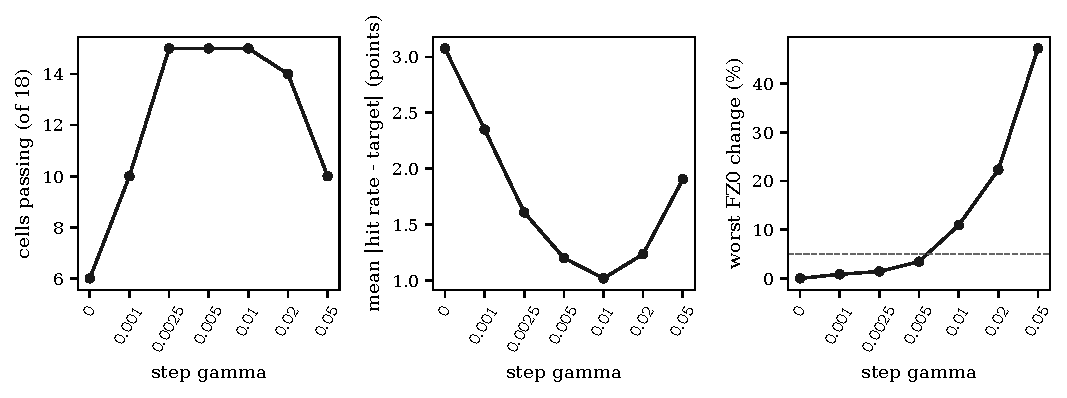
\includegraphics[width=\textwidth]{gamma-sweep}
\caption{Effect of the step $\gamma$ of the level update on HS-250, GARCH-t and FHS at two levels in the three stress windows (18 cells): cells passing the Kupiec and conditional coverage tests (left), mean distance of the hit rate from its target in percentage points (centre) and the worst relative change of the mean FZ0 score (right, the dashed line being the 5\% tolerance); the first point, 0, is the unwrapped model.}
\label{fig:gamma-sweep}
\end{figure}

\subsection{The band and the paired ES matter little at this scale}
\label{sec:ablation-band-es}

Widening the band to $[10^{-5}, 0.5]$ changes nothing in the count of cells passed (\ablBandWidePass{}) and leaves the worst score change at \ablBandWideFzWorst\%; the clipped days fall from \ablFullClip{} to \ablBandWideClip{}. Narrowing it to $[\alpha/2, 2\alpha]$ costs three cells (\ablBandNarrowPass{} passed) and raises the mean distance of the hit rate to \ablBandNarrowDev{} points, with \ablBandNarrowClip{} clipped days: a band that is too tight does not let the level reach the value at which the model is right, which is the content of \cref{prop:fixed-point}(c). The default band is therefore wide enough for these windows and need not be wider; no cell failed because of it, except in the scale sweep, where the band limits the repair (\cref{tab:scale-sweep}).

The two alternatives to the model's own tail mean as the ES do not change the coverage, as they should not (the VaR is the same), and change the ES calibration slightly: the mean $Z_2$ is \ablFullZtwo{} for the default, \ablEsRatioZtwo{} when the ES keeps the model's ratio to the VaR at the target level, and \ablEsTargetZtwo{} when it is left at the target level, with worst score changes of \ablEsRatioFzWorst\% and \ablEsTargetFzWorst\%. The differences are of the order of 0.1 in $Z_2$ and 0.6 percentage points in the score, and the experiment gives no interval for them; the decision to use the model's own ES at the working level rests on its coherence with the VaR (both come from one distribution) and not on a measured advantage.

\subsection{What each component contributes}
\label{sec:ablation-summary}

Reading the table as a decomposition, the update itself contributes the whole gain in cells passed: from \ablOffPass{} to \ablFullPass{} of \ablOffN{}, with no independence failure introduced (\ablFullInd{} failures against \ablOffInd{} unwrapped). The step sets how fast the gain is reached and how much score it costs, with an interior range of good values. The band bounds the repair and matters when it is too narrow. The paired ES is a matter of convention within the precision of these windows. None of the variants repairs the ES: the mean $Z_2$ stays between \ablEsRatioZtwo{} and \ablGammaAZtwo{} in all of them, against \ablOffZtwo{} for the unwrapped models.

Two limits of the decomposition follow from its design. The components were changed one at a time, so an interaction (a wider band with a larger step, say, which would let a fast level reach deeper before it is cut) was not measured. The counts of cells passed are counts over 18 cells that share the days of three windows, and a difference of one or two cells, such as the one between the steps 0.01 and 0.02, is within what a change of a few hits would move; the ordering of the steps is read from the pattern over the whole sweep of \cref{fig:gamma-sweep} and not from any single neighbouring pair.

\section{Discussion}
\label{sec:discussion}

\subsection{Why the repair works where it does}
\label{sec:discussion-why}

The wrapped models gain coverage in the stress windows because the stress windows are the case the update was built for: a regime in which the model understates the tail by a scale factor that persists for months. Historical simulation is the clearest example. Its window of 250 days still holds the calm year when the crisis begins, so its empirical quantile is a scale error of a factor that grows with the ratio of the crisis volatility to the calm volatility; the working level falls until the quantile of that old window reaches the new losses. The scale-sweep experiment says how far this can go: a scale error of 1.5 at the 1\% level is repaired in direction but not fully, because the fixed point lies close enough to the lower edge of the band that the spread of the level makes the band bind, and the identity of \cref{prop:identity} accounts for the excess of the hit rate to within 0.01 points. The models whose own filter follows the volatility (GARCH-t, FHS, the extreme-value model) have a smaller error to repair, gain fewer passes per cell, and at the 1\% level pay a small score cost, within the tolerance, a pattern consistent with a level that fluctuates around a fixed point that is already near the target.

That the independence test does not fail after the wrap is not a property of the method. \Cref{prop:independence} shows that it can fail with certainty on a sequence that the identity allows, and the stress windows contain few enough hits (between 2 and 17 per cell for the wrapped models of the main table) that the independence test has little power to reject. The result of the experiment is that the wrapper did not cause a rejection in \tenIndRunsAll{} runs, and that the unwrapped models had \tenIndFailUnwAll{} rejections of independence; neither number says that the wrapper repairs clustering. A smaller number of hits gives the independence statistic fewer pairs of consecutive hits to count, so a lower rate of hits may by itself lower the statistic without repairing any dependence.

\subsection{The failure cases}
\label{sec:discussion-failures}

Four failures are in the results and should be read as properties of the method. The delta-normal model gains no stress window at the 1\% level; it shares with the other models a hit rate that improves, and differs by a tail so thin that the working level sits at the band edge on \clipDnRollingOneEqCrisis{} days of the crisis window and the hits that remain fail the tests. The historical-simulation models still fail the Kupiec test at the 1\% level in the crisis window and at both levels in the pandemic window: a window of 104 days that contains a crash, with a level that needs about 100 quiet days to relax after one hit, is a case where the recalibration is late by construction. The wrapper does not repair the ES (the mean $Z_2$ remains negative), which is the consequence of paying no attention to the ES in the update and of the fact that the tails of the models are not Pareto (\cref{prop:es}). And for the models that already track volatility, the generator experiments show a loss of accuracy against the true VaR in \genErrWorseCells{} of \genErrWorseDen{} cells: the update trades some of the accuracy of a good estimate for the coverage of a bad one, and the supervisor's tests, which are on coverage, would not show the trade.

\subsection{What the comparison with other recalibrations implies}
\label{sec:discussion-comparison}

The comparison in \cref{sec:results-comparators} removes an easy conclusion. If the wrapper were the only way to move the coverage of a model towards its target, its gain in cells passed would be a property of the method; it is not, since a rolling split-conformal scale passes as many cells and a quantile tracker at a larger step passes more. The reason is that the repair of coverage under a persistent scale error is the common content of all these updates, which share the feature that a hit moves the working quantity one way and a quiet day the other. The differences between them are second-order: the rolling scale has no memory of the direction of its error and moves with the sample quantile of the last 250 scores, whose own noise at the 1\% level (the second largest of 250 scores, and the sixth largest at 2.5\%) moves the VaR by large factors, a plausible reason for its \cmpRollTenFzOver{} cells over the score tolerance, the worst of them in the short pandemic window where a crash lifts the scale to \cmpRollWorstScaleMax{}; the tracker has a step with the dimension of a score and a pass count that rises with it; the level wrapper keeps the VaR and the ES on one distribution and pays for the speed of its step in the score, as the ablation shows. What the wrapper offers a bank is not a larger number of passed windows but a recalibration that leaves the model's own distribution in charge of the ES, within a score tolerance, with a step that has a meaning in probability (a hit moves the level by $\gamma(1-\alpha)$). Whether that is worth a model of its own is a decision for the validator, and the data here do not make it.

\subsection{What a pass count measures}
\label{sec:discussion-passcount}

A bank reads a back-test as a binary outcome: the model passes or it does not. \Cref{sec:results-dispersion} shows that the outcome depends on the dispersion of the hit count as much as on its mean. The update ties the count of hits to its target through the identity of \cref{prop:identity}, whatever the model, and a count tied in this way is accepted by tests that assume independent hits. A validator who runs the Kupiec or the conditional coverage test on a recalibrated VaR therefore tests a null that the recalibration has changed, and the run passes more often than a correct unrecalibrated model would. The consequence is not specific to this wrapper: the rolling scale and the quantile tracker show a weaker under-dispersion in the generators (ratios \dispRatioRollMin{} to \dispRatioRollMax{} and \dispRatioTrkMin{} to \dispRatioTrkMax{}, against \dispRatioAciMin{} to \dispRatioAciMax{} for the wrapper), and a recalibration that feeds the hit back into the forecast can be expected to show it. Three readings follow. The hit rate and its distance from the target, which the tests do not enter, are the evidence of a repair that survives. The pass counts of a recalibrated model are to be read against a null simulated with the same recalibration, as in the recount of \cref{sec:results-dispersion}, where the gain falls from \tenPassAci{} against \tenPassUnw{} cells to \dispCWrapCal{} against \dispCUnwExact{}. And the supervisor's traffic light reads a count of exceptions and would, by the same argument, place a count held near its target in the green zone more often than a count of independent hits (the experiments tabulate hits, not zones, so this is not measured here), which is a reason to ask the bank for the recalibration rule and not only for the count.

\subsection{Implications for the validation of a bank's model}
\label{sec:discussion-implications}

A validator who finds that a model fails in a stress window has two instruments in hand after this work. The first is to read the wrapper as a diagnostic: the path of the working level, the days at the band edge and the mean level tell how far the model is from its target in scale. A model whose level sits at the lower edge for months, as the delta-normal model does, has an error that no step repairs; a model whose level moves by a few tenths of the target and returns has a localised failure. The second is the repair itself, for the models whose structure cannot be changed quickly. The repair does not substitute for the capital multiplier of the standard \citep{bcbs1996}, which rises with the count of exceedances over 250 days and is a consequence applied after the fact; it changes the VaR that produces the exceedances. A bank that adopts it would present to the supervisor the unwrapped model's back-test, the wrapped model's back-test, and the level path, since the supervisor reads the VaR that the bank reports and the reported VaR would be the wrapped one. The wrapper's dependence on realised losses of the day also means that a bank has to record the hit before the next day's forecast; the hit of a late-booked day is out of scope of the method and of its test.

\section{Limitations}
\label{sec:limitations}

\subsection{Internal validity}
\label{sec:limits-internal}

Each real window is one realised path. The intervals reported on the real windows (Wilson intervals of the hit rates, bootstrap intervals of the score change) describe the sampling variability of the days within the path, and not the variability of the crisis that produced it, so a window that is a single event cannot support a claim about the frequency with which the wrapper repairs coverage in crises in general; the generator experiments supply the replication, for a data-generating process chosen by the author. The windows are short: the pandemic window holds 104 days and 2 to 13 hits per cell in the unwrapped runs, and the Kupiec and conditional coverage p-values are asymptotic, which the engine documents as crude at counts of this size. A cell that passes or fails by a small margin (a p-value of 0.049 fails and 0.050 passes) is sensitive to one hit more or less; \cref{tab:main-results} shows several such cells, among them the wrapped HS-250 at the 1\% level in the crisis window and at the 2.5\% level in the pandemic window, whose conditional coverage p-values are both 0.055 and whose Kupiec p-values of 0.021 and 0.022 decide the fail. The count of passed cells is therefore a coarse summary, and the hit rates and score changes with their intervals are the better evidence. The hypothesis was written with a rule that counts windows passed; a different threshold of the p-value would change the counts.

The step and the band were fixed before the stress windows were run, and the other recalibrations were given constants fixed before their runs; but the choice of which recalibrations to compare, of the tracker's step grid and of the ablation grid was made after the first results on three models were known, and the sensitivity of the tracker to its step shows that the ranking of methods depends on that choice. The ten-model extension used the same constants as the three-model test. No multiplicity correction is applied to the \tenRuns{} cells.

\subsection{External validity}
\label{sec:limits-external}

The portfolios are public series (the US equity market, a ten-year Treasury position, the euro against the dollar) and three mixed portfolios with constant weights; a bank's portfolio has options, credit spreads and positions that change daily, and the VaR of a bank is computed from a full revaluation or a sensitivity model, not from the return series of a market index. The wrapper needs the model to answer at another level; for a bank's production model that is a commitment on its own, and for the five ladder models fitted for one level it requires a refit that the experiments do not test. The three models without an ES cannot be wrapped at all. The stress windows are the ones that Contraste chose, all of the 2000s and 2020s United States and euro markets; they contain neither a currency crisis of an emerging market nor a sovereign event. The tail levels are 1\% and 2.5\%; the supervisory ES level and the 99\% VaR of the older standard are the first of these, but the behaviour at 0.1\% is not tested, and at that level the band's lower edge of 0.001 leaves no room.

\subsection{Construct validity}
\label{sec:limits-construct}

The pass rule (Kupiec and conditional coverage both at least 0.05) is the product's, not the supervisor's: the Basel traffic light counts exceedances over 250 days and has its own zones \citep{bcbsmar32}: at the 1\% level it is green up to four exceptions and red from ten \citep{bcbs1996}, a reading by count alone that ignores the clustering the independence test sees. The experiments tabulate hits, not zones, so a statement that the wrapped models would have been in a lower zone is not made; and a window shorter than 250 days (the pandemic and the 2023 windows) has no zone at all. A bank that reads its record through the zones would therefore see the effect of the wrapper only through the count of hits that the main table gives. The score tolerance of 5\% is a decision. The FZ0 score is a consistent score for the pair, but it is one score among a family, and a different member could rank the recalibrations differently. The independence test of the engine has a first-order alternative and no power against dependence at longer lags, and the duration-based alternative of \citet{christoffersenpelletier2004} was not run. The ES is tested by the statistic of \cref{eq:z2} only; the more recent ES back-tests \citep{duescanciano2017,kratz2018,bayer2022,wang2022} were not run on the wrapped pair, and a wrapped ES may fail them for reasons that $Z_2$ does not see.

\subsection{Scope of the claims}
\label{sec:limits-scope}

The manuscript claims that, on ten ladder models and three stress windows, a wrapper with a pre-set step passes more cells than the unwrapped models without a score cost over 5\% and without an independence failure, that it holds on known-truth generators of persistent and transient shifts, and that its repair is bounded by the band and by the scale of the error. It does not claim the update as a novelty (it is the update of \citet{gibbs2021}); it does not claim to be better than the other recalibrations compared, and the results show that it is not better by cells passed; it does not claim to repair the ES or the independence; and it does not claim that its guarantee, which is vacuous at these window lengths, explains the empirical repair. The reproduction by an independent group on other portfolios is the test the claim has not had. The French equity series is distributed for derived use, so the equity returns cannot be redistributed with the code, and a reader needs the series from the library to rerun the equity windows.

\section{Reproducibility}
\label{sec:reproducibility}

The code, the committed forecasts and the scripts are in the repository named in the header block, under \texttt{manuscripts/adaptive-conformal-recalibration-of-var}. The results were produced with release v1.00.000 of CAOS\_Contraste (tag v1.00.000). The engine is \texttt{riskvalidation} 1.1.0, released on PyPI, with the extras for market risk, machine learning and stress tests, and the interpreter is Python 3.13 with \texttt{numpy} 2.4, \texttt{scipy} 1.18, \texttt{arch} 8.0 and \texttt{torch} 2.14 as pinned by the pipeline. The committed documents of the market case under \texttt{data/derived/C11} hold the forecasts of the ladder and the wrapped runs of the three models of the hypothesis. The raw series (the French library file, the Treasury par curves and the H.10 release) are read from the data root named by the environment variable \texttt{CONTRASTE\_DATA}; the French file is distributed for derived use only. % voice-ok: citation of the product release the results were produced with

Every number of the text is generated. The script \texttt{make\_numbers.py} writes \texttt{tables/numbers.tex}, which defines a macro for each quoted figure; \texttt{make\_tables.py} and \texttt{make\_figures.py} write the tables and the vector figures from the JSON outputs of the experiments, which are committed under \texttt{experiments/}. The experiments are run from the repository root:
\begin{description}
\item[\texttt{e2\_wrap\_ladder.py}] the wrapper on ten ladder models in six windows, with the reproduction of the committed rows (\reproEqual{} of \reproChecked{} rows equal to the committed documents, and the unwrapped runs of all ten models equal to the ladder's forecasts day by day); \texttt{python manuscripts/adaptive-conformal-recalibration-of-var/experiments/e2\_wrap\_ladder.py --workers 28 --cache \$CAOS\_TEMP\_ROOT/contraste-adaptive-conformal/cache}, with \texttt{CONTRASTE\_DATA} set;
\item[\texttt{e3\_ablation.py}] the ablation of \cref{tab:ablation}; \texttt{python manuscripts/adaptive-conformal-recalibration-of-var/experiments/e3\_ablation.py --workers 28 --returns-cache \$CAOS\_TEMP\_ROOT/contraste-adaptive-conformal/windows.npz}, with \texttt{CONTRASTE\_DATA} set;
\item[\texttt{e4\_score\_space.py}] the two score-space recalibrations on all eighteen models; \texttt{python manuscripts/adaptive-conformal-recalibration-of-var/experiments/e4\_score\_space.py --returns-cache \$CAOS\_TEMP\_ROOT/contraste-adaptive-conformal/windows.npz}, with \texttt{CONTRASTE\_DATA} set;
\item[\texttt{check\_e4\_baseline.py}] the consistency check of the previous output: the unwrapped baseline of experiment 4 equals that of experiment 2 and the committed documents; \texttt{python manuscripts/adaptive-conformal-recalibration-of-var/experiments/check\_e4\_baseline.py};
\item[\texttt{e5\_generators.py}] the generators of known truth, 100 replications of four scenarios, the seed of replication $k$ of scenario $s$ being \seedBase{} plus $1000s + k$; \texttt{python manuscripts/adaptive-conformal-recalibration-of-var/experiments/e5\_generators.py --workers 28};
\item[\texttt{e6\_theory.py}] the numerical checks of the propositions: the identity on the 18 real level paths, the clustered sequences, the scale sweep with 50 replications of 5,000 days (seed \seedBase{} plus 777000 plus the replication) and the ES ratios; \texttt{python manuscripts/adaptive-conformal-recalibration-of-var/experiments/e6\_theory.py};
\item[\texttt{e7\_dispersion.py}] the dispersion of the hit count and the size of the tests on wrapped runs (\cref{sec:results-dispersion}); \texttt{python manuscripts/adaptive-conformal-recalibration-of-var/experiments/e7\_dispersion.py}; it reads \texttt{e2\_wrap\_ladder.json} and \texttt{e5\_generators.json}, and its own draws use \texttt{default\_rng} with the seed list \seedBase{}, 7 or 8, and the indices of the row.
\end{description}
The scripts \texttt{make\_numbers.py}, \texttt{make\_tables.py} and \texttt{make\_figures.py} are run from the repository root without arguments after the experiments.
The bootstrap uses circular blocks of 10 days and 2,000 draws with the seed \seedBase{} plus a fixed integer per window, model and level. The cost of the experiments was measured on a workstation with 32 logical cores: the wrapped runs of ten models in six windows (the heavy part is the daily refit of the GARCH, GJR, EGARCH and extreme-value models) took 168 seconds of wall time with 28 worker processes from an empty run cache. The ablation took 439 seconds, the score-space recalibrations 130 seconds and the generators 176 seconds in a first run, and 90, 16 and 31 seconds in a repeat that reused the cached parsed returns and fits, the times each script records in its output; the numerical checks of the theory took 613 seconds, measured outside the script. A repeat of experiments 2, 3, 5 and 6 reproduces the stored outputs. The score-space recalibrations take 32 seconds, and \texttt{check\_e4\_baseline.py} verifies that each comparator run scores the pair of its own VaR and ES; the dispersion experiment takes under two minutes. Each script finishes in under 30 minutes. The step of the wrapper, 0.005, and the band, $[0.001, 0.25]$, are the defaults of the engine and appear nowhere else as parameters.

The numerical checks of the theory are part of these scripts. The identity of \cref{prop:identity} holds on the 18 real level paths with a largest residual of $\thAResidual$ and the bound holds on \thAHold{} of \thA{}; the clustered sequences of \cref{tab:cluster} are tested with the engine's own tests; the scale sweep of \cref{tab:scale-sweep} is a simulation with the stated seeds; and the ES ratios of \cref{prop:es} are computed in closed form from the Student-$t$ law. A reader who runs the figure and table scripts from the committed JSON obtains the same files without the raw series; a reader who reruns the experiments needs the series and obtains the same numbers to the last digit of the stored JSON, because no step draws a random number except through the stated seeds.

\section{Conclusions}
\label{sec:conclusions}

Wrapping a value-at-risk model in an adaptive conformal update of its tail level improves its coverage in market stress. On ten of the eighteen models of the ladder and three stress windows, the wrapped models pass the Kupiec and conditional coverage tests in \tenPassAci{} of \tenRuns{} model-level-window cells against \tenPassUnw{} unwrapped. The prediction stated before the runs holds: HS-250, GARCH-t and filtered historical simulation each gain at least one stress window at both levels (\hypCellsHold{} of \hypCells{} cells), the worst change of the mean score is \hypWorstFz\%, below the 5\% tolerance, and the independence test is not failed in the crisis window (p-values \indMin{} to \indMax{}). On generators of known truth the wrapped pass rate is higher in all \genPredANum{} cells with a shift.

The result has limits that the experiments and the theory give numbers for. The guarantee on the long-run frequency of hits is vacuous at the length of a stress window (the bound averages \thAMeanSimple{} percentage points), so the repair is an empirical result; the repair is bounded by the band and by the scale of the model's error (a ratio of \thCCmaxOne{} at the 1\% level for a Student-$t$ model with five degrees of freedom), and the band binds the level well before the fixed point leaves it; a coverage guarantee carries no independence (\cref{prop:independence}); the expected shortfall remains understated (mean $Z_2$ \tenMeanZtwoAci{} wrapped against \tenMeanZtwoUnw{}); the delta-normal model gains no window at the 1\% level; and for volatility-filtered models the wrapper lowers the accuracy of the VaR against the truth in most generator cells. Two other recalibrations that act on the finished VaR pass as many cells (a rolling split-conformal scale, at a cost in the score) or more (a quantile tracker with a larger step, also at a cost), so the wrapper is one of several methods that move coverage, distinguished by keeping the model's own ES at the working level and by a step that has a probabilistic meaning.

The next steps are the tests the claim has not had: portfolios with options and spreads, the models fitted for one level through a refit at the working level, the ES back-tests of the recent literature on the wrapped pair, windows of other markets, and a selection of the step by a rule that does not use the windows on which the wrapper is judged.


\bibliographystyle{plainnat}
\bibliography{references}

\end{document}
